\documentclass[a4paper]{book}
\usepackage{makeidx}
\usepackage{graphicx}
\usepackage{multicol}
\usepackage{float}
\usepackage{listings}
\usepackage{color}
\usepackage{ifthen}
\usepackage[table]{xcolor}
\usepackage{textcomp}
\usepackage{alltt}
\usepackage{ifpdf}
\ifpdf
\usepackage[pdftex,
            pagebackref=true,
            colorlinks=true,
            linkcolor=blue,
            unicode
           ]{hyperref}
\else
\usepackage[ps2pdf,
            pagebackref=true,
            colorlinks=true,
            linkcolor=blue,
            unicode
           ]{hyperref}
\usepackage{pspicture}
\fi
\usepackage[utf8]{inputenc}
\usepackage{mathptmx}
\usepackage[scaled=.90]{helvet}
\usepackage{courier}
\usepackage{sectsty}
\usepackage[titles]{tocloft}
\usepackage{doxygen}
\lstset{language=C++,inputencoding=utf8,basicstyle=\footnotesize,breaklines=true,breakatwhitespace=true,tabsize=4,numbers=left }
\makeindex
\setcounter{tocdepth}{3}
\renewcommand{\footrulewidth}{0.4pt}
\renewcommand{\familydefault}{\sfdefault}
\begin{document}
\hypersetup{pageanchor=false}
\begin{titlepage}
\vspace*{7cm}
\begin{center}
{\Large RHeroes }\\
\vspace*{1cm}
{\large Generated by Doxygen 1.7.4}\\
\vspace*{0.5cm}
{\small Sun Nov 27 2011 02:15:00}\\
\end{center}
\end{titlepage}
\clearemptydoublepage
\pagenumbering{roman}
\tableofcontents
\clearemptydoublepage
\pagenumbering{arabic}
\hypersetup{pageanchor=true}
\chapter{Namespace Index}
\section{Namespace List}
Here is a list of all namespaces with brief descriptions:\begin{DoxyCompactList}
\item\contentsline{section}{\hyperlink{namespaceUi}{Ui} }{\pageref{namespaceUi}}{}
\end{DoxyCompactList}

\chapter{Class Index}
\section{Class Hierarchy}
This inheritance list is sorted roughly, but not completely, alphabetically:\begin{DoxyCompactList}
\item \contentsline{section}{AbstractSocketController}{\pageref{classAbstractSocketController}}{}
\begin{DoxyCompactList}
\item \contentsline{section}{UPISController}{\pageref{classUPISController}}{}
\item \contentsline{section}{USARController}{\pageref{classUSARController}}{}
\end{DoxyCompactList}
\item \contentsline{section}{Action}{\pageref{classAction}}{}
\item \contentsline{section}{BaseStation}{\pageref{classBaseStation}}{}
\item \contentsline{section}{BaseStationUi}{\pageref{classBaseStationUi}}{}
\item \contentsline{section}{Driver}{\pageref{classDriver}}{}
\item \contentsline{section}{Message}{\pageref{classMessage}}{}
\begin{DoxyCompactList}
\item \contentsline{section}{CameraData}{\pageref{classCameraData}}{}
\item \contentsline{section}{LaserData}{\pageref{classLaserData}}{}
\item \contentsline{section}{OdometryData}{\pageref{classOdometryData}}{}
\item \contentsline{section}{UPISMessage}{\pageref{classUPISMessage}}{}
\item \contentsline{section}{USARMessage}{\pageref{classUSARMessage}}{}
\end{DoxyCompactList}
\item \contentsline{section}{Pose}{\pageref{classPose}}{}
\item \contentsline{section}{Robot}{\pageref{classRobot}}{}
\item \contentsline{section}{RobotController}{\pageref{classRobotController}}{}
\item \contentsline{section}{RobotState}{\pageref{classRobotState}}{}
\item \contentsline{section}{RobotUi}{\pageref{classRobotUi}}{}
\item \contentsline{section}{Sensor}{\pageref{classSensor}}{}
\begin{DoxyCompactList}
\item \contentsline{section}{CameraSensor}{\pageref{classCameraSensor}}{}
\item \contentsline{section}{LaserSensor}{\pageref{classLaserSensor}}{}
\item \contentsline{section}{OdometrySensor}{\pageref{classOdometrySensor}}{}
\end{DoxyCompactList}
\item \contentsline{section}{SensorData}{\pageref{classSensorData}}{}
\end{DoxyCompactList}

\chapter{Class Index}
\section{Class List}
Here are the classes, structs, unions and interfaces with brief descriptions:\begin{DoxyCompactList}
\item\contentsline{section}{\hyperlink{classAbstractSocketController}{AbstractSocketController} (Shared functionalities for socket based controllers )}{\pageref{classAbstractSocketController}}{}
\item\contentsline{section}{\hyperlink{classAction}{Action} }{\pageref{classAction}}{}
\item\contentsline{section}{\hyperlink{classBaseStation}{BaseStation} }{\pageref{classBaseStation}}{}
\item\contentsline{section}{\hyperlink{classBaseStationUi}{BaseStationUi} }{\pageref{classBaseStationUi}}{}
\item\contentsline{section}{\hyperlink{classCameraData}{CameraData} (Camera data message )}{\pageref{classCameraData}}{}
\item\contentsline{section}{\hyperlink{classCameraSensor}{CameraSensor} (\hyperlink{classSensor}{Sensor} for camera data )}{\pageref{classCameraSensor}}{}
\item\contentsline{section}{\hyperlink{classDriver}{Driver} (Generic driver interface )}{\pageref{classDriver}}{}
\item\contentsline{section}{\hyperlink{classLaserData}{LaserData} (Laser data message )}{\pageref{classLaserData}}{}
\item\contentsline{section}{\hyperlink{classLaserSensor}{LaserSensor} (\hyperlink{classSensor}{Sensor} for laser scans )}{\pageref{classLaserSensor}}{}
\item\contentsline{section}{\hyperlink{classMessage}{Message} (Generic message container )}{\pageref{classMessage}}{}
\item\contentsline{section}{\hyperlink{classOdometryData}{OdometryData} (Odometric data message )}{\pageref{classOdometryData}}{}
\item\contentsline{section}{\hyperlink{classOdometrySensor}{OdometrySensor} (\hyperlink{classSensor}{Sensor} for odometric data )}{\pageref{classOdometrySensor}}{}
\item\contentsline{section}{\hyperlink{classPose}{Pose} }{\pageref{classPose}}{}
\item\contentsline{section}{\hyperlink{classRobot}{Robot} }{\pageref{classRobot}}{}
\item\contentsline{section}{\hyperlink{classRobotController}{RobotController} }{\pageref{classRobotController}}{}
\item\contentsline{section}{\hyperlink{classRobotState}{RobotState} }{\pageref{classRobotState}}{}
\item\contentsline{section}{\hyperlink{classRobotUi}{RobotUi} }{\pageref{classRobotUi}}{}
\item\contentsline{section}{\hyperlink{classSensor}{Sensor} (Generic sensor interface )}{\pageref{classSensor}}{}
\item\contentsline{section}{\hyperlink{classSensorData}{SensorData} }{\pageref{classSensorData}}{}
\item\contentsline{section}{\hyperlink{classUPISController}{UPISController} (UPIS connection controller )}{\pageref{classUPISController}}{}
\item\contentsline{section}{\hyperlink{classUPISMessage}{UPISMessage} (\hyperlink{classMessage}{Message} representing data sent from UPIS )}{\pageref{classUPISMessage}}{}
\item\contentsline{section}{\hyperlink{classUSARController}{USARController} (USARSim connection controller )}{\pageref{classUSARController}}{}
\item\contentsline{section}{\hyperlink{classUSARMessage}{USARMessage} (\hyperlink{classMessage}{Message} representing data sent to and from USARSim )}{\pageref{classUSARMessage}}{}
\end{DoxyCompactList}

\chapter{File Index}
\section{File List}
Here is a list of all files with brief descriptions:\begin{DoxyCompactList}
\item\contentsline{section}{\hyperlink{main_8cpp}{main.cpp} }{\pageref{main_8cpp}}{}
\item\contentsline{section}{connection/\hyperlink{abstractsocketcontroller_8cpp}{abstractsocketcontroller.cpp} }{\pageref{abstractsocketcontroller_8cpp}}{}
\item\contentsline{section}{connection/\hyperlink{abstractsocketcontroller_8h}{abstractsocketcontroller.h} }{\pageref{abstractsocketcontroller_8h}}{}
\item\contentsline{section}{connection/\hyperlink{upiscontroller_8cpp}{upiscontroller.cpp} }{\pageref{upiscontroller_8cpp}}{}
\item\contentsline{section}{connection/\hyperlink{upiscontroller_8h}{upiscontroller.h} }{\pageref{upiscontroller_8h}}{}
\item\contentsline{section}{connection/\hyperlink{usarcontroller_8cpp}{usarcontroller.cpp} }{\pageref{usarcontroller_8cpp}}{}
\item\contentsline{section}{connection/\hyperlink{usarcontroller_8h}{usarcontroller.h} }{\pageref{usarcontroller_8h}}{}
\item\contentsline{section}{data/\hyperlink{action_8cpp}{action.cpp} }{\pageref{action_8cpp}}{}
\item\contentsline{section}{data/\hyperlink{action_8h}{action.h} }{\pageref{action_8h}}{}
\item\contentsline{section}{data/\hyperlink{cameradata_8cpp}{cameradata.cpp} }{\pageref{cameradata_8cpp}}{}
\item\contentsline{section}{data/\hyperlink{cameradata_8h}{cameradata.h} }{\pageref{cameradata_8h}}{}
\item\contentsline{section}{data/\hyperlink{laserdata_8cpp}{laserdata.cpp} }{\pageref{laserdata_8cpp}}{}
\item\contentsline{section}{data/\hyperlink{laserdata_8h}{laserdata.h} }{\pageref{laserdata_8h}}{}
\item\contentsline{section}{data/\hyperlink{message_8h}{message.h} }{\pageref{message_8h}}{}
\item\contentsline{section}{data/\hyperlink{odometrydata_8cpp}{odometrydata.cpp} }{\pageref{odometrydata_8cpp}}{}
\item\contentsline{section}{data/\hyperlink{odometrydata_8h}{odometrydata.h} }{\pageref{odometrydata_8h}}{}
\item\contentsline{section}{data/\hyperlink{pose_8cpp}{pose.cpp} }{\pageref{pose_8cpp}}{}
\item\contentsline{section}{data/\hyperlink{pose_8h}{pose.h} }{\pageref{pose_8h}}{}
\item\contentsline{section}{data/\hyperlink{robotstate_8cpp}{robotstate.cpp} }{\pageref{robotstate_8cpp}}{}
\item\contentsline{section}{data/\hyperlink{robotstate_8h}{robotstate.h} }{\pageref{robotstate_8h}}{}
\item\contentsline{section}{data/\hyperlink{sensordata_8h}{sensordata.h} }{\pageref{sensordata_8h}}{}
\item\contentsline{section}{data/\hyperlink{upismessage_8cpp}{upismessage.cpp} }{\pageref{upismessage_8cpp}}{}
\item\contentsline{section}{data/\hyperlink{upismessage_8h}{upismessage.h} }{\pageref{upismessage_8h}}{}
\item\contentsline{section}{data/\hyperlink{usarmessage_8cpp}{usarmessage.cpp} }{\pageref{usarmessage_8cpp}}{}
\item\contentsline{section}{data/\hyperlink{usarmessage_8h}{usarmessage.h} }{\pageref{usarmessage_8h}}{}
\item\contentsline{section}{graphics/\hyperlink{basestationui_8cpp}{basestationui.cpp} }{\pageref{basestationui_8cpp}}{}
\item\contentsline{section}{graphics/\hyperlink{basestationui_8h}{basestationui.h} }{\pageref{basestationui_8h}}{}
\item\contentsline{section}{graphics/\hyperlink{robotui_8cpp}{robotui.cpp} }{\pageref{robotui_8cpp}}{}
\item\contentsline{section}{graphics/\hyperlink{robotui_8h}{robotui.h} }{\pageref{robotui_8h}}{}
\item\contentsline{section}{logic/\hyperlink{basestation_8cpp}{basestation.cpp} }{\pageref{basestation_8cpp}}{}
\item\contentsline{section}{logic/\hyperlink{basestation_8h}{basestation.h} }{\pageref{basestation_8h}}{}
\item\contentsline{section}{logic/\hyperlink{robot_8cpp}{robot.cpp} }{\pageref{robot_8cpp}}{}
\item\contentsline{section}{logic/\hyperlink{robot_8h}{robot.h} }{\pageref{robot_8h}}{}
\item\contentsline{section}{logic/\hyperlink{robotcontroller_8cpp}{robotcontroller.cpp} }{\pageref{robotcontroller_8cpp}}{}
\item\contentsline{section}{logic/\hyperlink{robotcontroller_8h}{robotcontroller.h} }{\pageref{robotcontroller_8h}}{}
\item\contentsline{section}{middleware/driver/\hyperlink{driver_8cpp}{driver.cpp} }{\pageref{driver_8cpp}}{}
\item\contentsline{section}{middleware/driver/\hyperlink{driver_8h}{driver.h} }{\pageref{driver_8h}}{}
\item\contentsline{section}{middleware/sensor/\hyperlink{camerasensor_8cpp}{camerasensor.cpp} }{\pageref{camerasensor_8cpp}}{}
\item\contentsline{section}{middleware/sensor/\hyperlink{camerasensor_8h}{camerasensor.h} }{\pageref{camerasensor_8h}}{}
\item\contentsline{section}{middleware/sensor/\hyperlink{lasersensor_8cpp}{lasersensor.cpp} }{\pageref{lasersensor_8cpp}}{}
\item\contentsline{section}{middleware/sensor/\hyperlink{lasersensor_8h}{lasersensor.h} }{\pageref{lasersensor_8h}}{}
\item\contentsline{section}{middleware/sensor/\hyperlink{odometrysensor_8cpp}{odometrysensor.cpp} }{\pageref{odometrysensor_8cpp}}{}
\item\contentsline{section}{middleware/sensor/\hyperlink{odometrysensor_8h}{odometrysensor.h} }{\pageref{odometrysensor_8h}}{}
\item\contentsline{section}{middleware/sensor/\hyperlink{sensor_8cpp}{sensor.cpp} }{\pageref{sensor_8cpp}}{}
\item\contentsline{section}{middleware/sensor/\hyperlink{sensor_8h}{sensor.h} }{\pageref{sensor_8h}}{}
\item\contentsline{section}{shared/\hyperlink{constants_8h}{constants.h} }{\pageref{constants_8h}}{}
\item\contentsline{section}{shared/\hyperlink{utilities_8h}{utilities.h} }{\pageref{utilities_8h}}{}
\end{DoxyCompactList}

\chapter{Namespace Documentation}
\hypertarget{namespaceUi}{
\section{Ui Namespace Reference}
\label{namespaceUi}\index{Ui@{Ui}}
}

\chapter{Class Documentation}
\hypertarget{classAbstractSocketController}{
\section{AbstractSocketController Class Reference}
\label{classAbstractSocketController}\index{AbstractSocketController@{AbstractSocketController}}
}


Shared functionalities for socket based controllers.  




{\ttfamily \#include $<$abstractsocketcontroller.h$>$}

Inheritance diagram for AbstractSocketController:\begin{figure}[H]
\begin{center}
\leavevmode
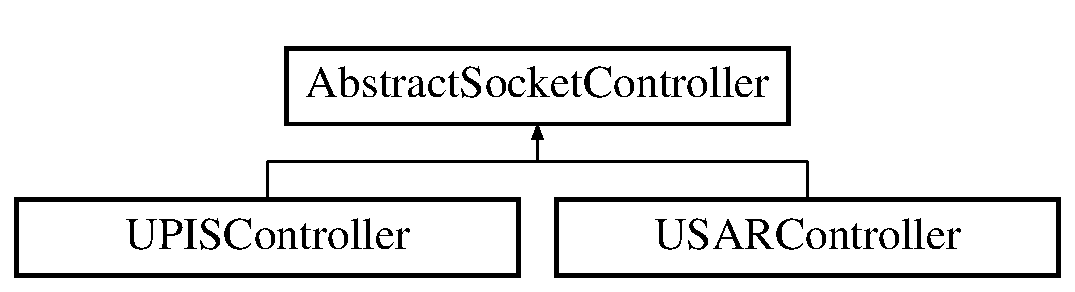
\includegraphics[height=2.000000cm]{classAbstractSocketController}
\end{center}
\end{figure}
\subsection*{Public Slots}
\begin{DoxyCompactItemize}
\item 
virtual void \hyperlink{classAbstractSocketController_a13af2e22144c96860f6a3975365dc1ff}{connectToHost} (const QString \&address, quint16 port)
\item 
virtual void \hyperlink{classAbstractSocketController_a399c565654a03e6cb352dfc576460ff7}{disconnectFromHost} ()
\end{DoxyCompactItemize}
\subsection*{Signals}
\begin{DoxyCompactItemize}
\item 
void \hyperlink{classAbstractSocketController_af09d800cea400d85c29e07322faaf934}{signalConnected} ()
\item 
void \hyperlink{classAbstractSocketController_afc064b05ae1963fc4741d61c49e9b6ad}{signalError} (const QString \&msg)
\item 
void \hyperlink{classAbstractSocketController_a5d1dee9948125660e67a671cabed122f}{signalDisconnected} ()
\end{DoxyCompactItemize}
\subsection*{Public Member Functions}
\begin{DoxyCompactItemize}
\item 
virtual \hyperlink{classAbstractSocketController_a62f22568654956a18a108f81ca18cda5}{$\sim$AbstractSocketController} ()
\end{DoxyCompactItemize}
\subsection*{Protected Slots}
\begin{DoxyCompactItemize}
\item 
virtual void \hyperlink{classAbstractSocketController_a3816ceb3b12f0028dea99d010349ec41}{invokeReadData} ()=0
\end{DoxyCompactItemize}
\subsection*{Protected Member Functions}
\begin{DoxyCompactItemize}
\item 
\hyperlink{classAbstractSocketController_a1e51beb8c90ce4f69a57d6464812f177}{AbstractSocketController} (QObject $\ast$parent=0)
\end{DoxyCompactItemize}
\subsection*{Protected Attributes}
\begin{DoxyCompactItemize}
\item 
QTcpSocket $\ast$ \hyperlink{classAbstractSocketController_aa979beef2f78be052f3e7f3255cdc644}{socket}
\end{DoxyCompactItemize}


\subsection{Detailed Description}
Shared functionalities for socket based controllers. 

\hyperlink{classAbstractSocketController}{AbstractSocketController} is a class that holds the methods and functionalities shared by controllers based on socket connections

\begin{DoxySeeAlso}{See also}
\hyperlink{classUSARController}{USARController} 

\hyperlink{classUPISController}{UPISController} 

WSSController 
\end{DoxySeeAlso}


\subsection{Constructor \& Destructor Documentation}
\hypertarget{classAbstractSocketController_a1e51beb8c90ce4f69a57d6464812f177}{
\index{AbstractSocketController@{AbstractSocketController}!AbstractSocketController@{AbstractSocketController}}
\index{AbstractSocketController@{AbstractSocketController}!AbstractSocketController@{AbstractSocketController}}
\subsubsection[{AbstractSocketController}]{\setlength{\rightskip}{0pt plus 5cm}AbstractSocketController::AbstractSocketController (
\begin{DoxyParamCaption}
\item[{QObject $\ast$}]{parent = {\ttfamily 0}}
\end{DoxyParamCaption}
)\hspace{0.3cm}{\ttfamily  \mbox{[}explicit, protected\mbox{]}}}}
\label{classAbstractSocketController_a1e51beb8c90ce4f69a57d6464812f177}
Constructs a new \hyperlink{classAbstractSocketController}{AbstractSocketController}


\begin{DoxyParams}{Parameters}
{\em parent} & Optional QObject parent \\
\hline
\end{DoxyParams}
\hypertarget{classAbstractSocketController_a62f22568654956a18a108f81ca18cda5}{
\index{AbstractSocketController@{AbstractSocketController}!$\sim$AbstractSocketController@{$\sim$AbstractSocketController}}
\index{$\sim$AbstractSocketController@{$\sim$AbstractSocketController}!AbstractSocketController@{AbstractSocketController}}
\subsubsection[{$\sim$AbstractSocketController}]{\setlength{\rightskip}{0pt plus 5cm}AbstractSocketController::$\sim$AbstractSocketController (
\begin{DoxyParamCaption}
{}
\end{DoxyParamCaption}
)\hspace{0.3cm}{\ttfamily  \mbox{[}virtual\mbox{]}}}}
\label{classAbstractSocketController_a62f22568654956a18a108f81ca18cda5}
Destroys the \hyperlink{classAbstractSocketController}{AbstractSocketController} 

\subsection{Member Function Documentation}
\hypertarget{classAbstractSocketController_a13af2e22144c96860f6a3975365dc1ff}{
\index{AbstractSocketController@{AbstractSocketController}!connectToHost@{connectToHost}}
\index{connectToHost@{connectToHost}!AbstractSocketController@{AbstractSocketController}}
\subsubsection[{connectToHost}]{\setlength{\rightskip}{0pt plus 5cm}void AbstractSocketController::connectToHost (
\begin{DoxyParamCaption}
\item[{const QString \&}]{address, }
\item[{quint16}]{port}
\end{DoxyParamCaption}
)\hspace{0.3cm}{\ttfamily  \mbox{[}virtual, slot\mbox{]}}}}
\label{classAbstractSocketController_a13af2e22144c96860f6a3975365dc1ff}
Establishes a connection to the specified host/port. This method is non-\/blocking, hence, before any communication is attempted the application should wait for the \hyperlink{classAbstractSocketController_af09d800cea400d85c29e07322faaf934}{signalConnected()} signal


\begin{DoxyParams}{Parameters}
{\em address} & IP address or hostname of the target host \\
\hline
{\em port} & TCP port to connect to \\
\hline
\end{DoxyParams}


Reimplemented in \hyperlink{classUPISController_a78dcb22bf16cca05bebd9dd923c7ba28}{UPISController}.

\hypertarget{classAbstractSocketController_a399c565654a03e6cb352dfc576460ff7}{
\index{AbstractSocketController@{AbstractSocketController}!disconnectFromHost@{disconnectFromHost}}
\index{disconnectFromHost@{disconnectFromHost}!AbstractSocketController@{AbstractSocketController}}
\subsubsection[{disconnectFromHost}]{\setlength{\rightskip}{0pt plus 5cm}void AbstractSocketController::disconnectFromHost (
\begin{DoxyParamCaption}
{}
\end{DoxyParamCaption}
)\hspace{0.3cm}{\ttfamily  \mbox{[}virtual, slot\mbox{]}}}}
\label{classAbstractSocketController_a399c565654a03e6cb352dfc576460ff7}
Terminates the connection to the host. The actual disconnection notification is emitted through the \hyperlink{classAbstractSocketController_a5d1dee9948125660e67a671cabed122f}{signalDisconnected()} signal 

Reimplemented in \hyperlink{classUPISController_a5d09ac4efcf74e202c905bf195f029dc}{UPISController}.

\hypertarget{classAbstractSocketController_a3816ceb3b12f0028dea99d010349ec41}{
\index{AbstractSocketController@{AbstractSocketController}!invokeReadData@{invokeReadData}}
\index{invokeReadData@{invokeReadData}!AbstractSocketController@{AbstractSocketController}}
\subsubsection[{invokeReadData}]{\setlength{\rightskip}{0pt plus 5cm}virtual void AbstractSocketController::invokeReadData (
\begin{DoxyParamCaption}
{}
\end{DoxyParamCaption}
)\hspace{0.3cm}{\ttfamily  \mbox{[}protected, pure virtual, slot\mbox{]}}}}
\label{classAbstractSocketController_a3816ceb3b12f0028dea99d010349ec41}
This slot should be implemented by subclasses. The slot is called every time new data is available in the input buffer 

Implemented in \hyperlink{classUPISController_a20c811385172668d1071f267cc52c559}{UPISController}, and \hyperlink{classUSARController_aea2a9dde924c625b83da33a6848f41f0}{USARController}.

\hypertarget{classAbstractSocketController_af09d800cea400d85c29e07322faaf934}{
\index{AbstractSocketController@{AbstractSocketController}!signalConnected@{signalConnected}}
\index{signalConnected@{signalConnected}!AbstractSocketController@{AbstractSocketController}}
\subsubsection[{signalConnected}]{\setlength{\rightskip}{0pt plus 5cm}void AbstractSocketController::signalConnected (
\begin{DoxyParamCaption}
{}
\end{DoxyParamCaption}
)\hspace{0.3cm}{\ttfamily  \mbox{[}signal\mbox{]}}}}
\label{classAbstractSocketController_af09d800cea400d85c29e07322faaf934}
This signal is emitted once the connection has been successfully established \hypertarget{classAbstractSocketController_a5d1dee9948125660e67a671cabed122f}{
\index{AbstractSocketController@{AbstractSocketController}!signalDisconnected@{signalDisconnected}}
\index{signalDisconnected@{signalDisconnected}!AbstractSocketController@{AbstractSocketController}}
\subsubsection[{signalDisconnected}]{\setlength{\rightskip}{0pt plus 5cm}void AbstractSocketController::signalDisconnected (
\begin{DoxyParamCaption}
{}
\end{DoxyParamCaption}
)\hspace{0.3cm}{\ttfamily  \mbox{[}signal\mbox{]}}}}
\label{classAbstractSocketController_a5d1dee9948125660e67a671cabed122f}
This signal is emitted once the connection has been successfully terminated \hypertarget{classAbstractSocketController_afc064b05ae1963fc4741d61c49e9b6ad}{
\index{AbstractSocketController@{AbstractSocketController}!signalError@{signalError}}
\index{signalError@{signalError}!AbstractSocketController@{AbstractSocketController}}
\subsubsection[{signalError}]{\setlength{\rightskip}{0pt plus 5cm}void AbstractSocketController::signalError (
\begin{DoxyParamCaption}
\item[{const QString \&}]{msg}
\end{DoxyParamCaption}
)\hspace{0.3cm}{\ttfamily  \mbox{[}signal\mbox{]}}}}
\label{classAbstractSocketController_afc064b05ae1963fc4741d61c49e9b6ad}
This signal is emitted in case an error happens


\begin{DoxyParams}{Parameters}
{\em msg} & The formatted error message \\
\hline
\end{DoxyParams}


\subsection{Member Data Documentation}
\hypertarget{classAbstractSocketController_aa979beef2f78be052f3e7f3255cdc644}{
\index{AbstractSocketController@{AbstractSocketController}!socket@{socket}}
\index{socket@{socket}!AbstractSocketController@{AbstractSocketController}}
\subsubsection[{socket}]{\setlength{\rightskip}{0pt plus 5cm}QTcpSocket$\ast$ {\bf AbstractSocketController::socket}\hspace{0.3cm}{\ttfamily  \mbox{[}protected\mbox{]}}}}
\label{classAbstractSocketController_aa979beef2f78be052f3e7f3255cdc644}
The actual socket used for connections, left protected for subclass convenience 

The documentation for this class was generated from the following files:\begin{DoxyCompactItemize}
\item 
connection/\hyperlink{abstractsocketcontroller_8h}{abstractsocketcontroller.h}\item 
connection/\hyperlink{abstractsocketcontroller_8cpp}{abstractsocketcontroller.cpp}\end{DoxyCompactItemize}

\hypertarget{classAction}{
\section{Action Class Reference}
\label{classAction}\index{Action@{Action}}
}


{\ttfamily \#include $<$action.h$>$}

\subsection*{Public Types}
\begin{DoxyCompactItemize}
\item 
enum \hyperlink{classAction_ab1851cee70a9061c928e69d44e6cba0b}{ActionType} \{ \hyperlink{classAction_ab1851cee70a9061c928e69d44e6cba0bab3f4515fff89bb5cc4c35a143e7d949a}{Rotation} =  0, 
\hyperlink{classAction_ab1851cee70a9061c928e69d44e6cba0bae6fc2e20d912178bcd386432c8443e99}{Translation} =  1
 \}
\end{DoxyCompactItemize}
\subsection*{Public Member Functions}
\begin{DoxyCompactItemize}
\item 
\hyperlink{classAction_ac04621d251f1465cac23501f906de535}{Action} (\hyperlink{classAction_ab1851cee70a9061c928e69d44e6cba0b}{ActionType} aType, double aValue)
\item 
\hyperlink{classAction_a4f457ccfc8336b565cadca56b36e0271}{Action} ()
\item 
virtual \hyperlink{classAction_acdb06775d157339256a8ecd55749226c}{$\sim$Action} ()
\item 
\hyperlink{classAction_ab1851cee70a9061c928e69d44e6cba0b}{ActionType} \hyperlink{classAction_a4228bc3ace4c7ff787440a773e82a7a9}{getType} () const 
\item 
double \hyperlink{classAction_ae342d376e783c930a80a580d5a7ab5f5}{getValue} () const 
\item 
void \hyperlink{classAction_a77869bc712f6079e6481a81a135a4dc4}{setType} (\hyperlink{classAction_ab1851cee70a9061c928e69d44e6cba0b}{ActionType} aType)
\item 
void \hyperlink{classAction_a67959f7849af9e06f6b033522adfadc8}{setValue} (double aValue)
\end{DoxyCompactItemize}


\subsection{Member Enumeration Documentation}
\hypertarget{classAction_ab1851cee70a9061c928e69d44e6cba0b}{
\index{Action@{Action}!ActionType@{ActionType}}
\index{ActionType@{ActionType}!Action@{Action}}
\subsubsection[{ActionType}]{\setlength{\rightskip}{0pt plus 5cm}enum {\bf Action::ActionType}}}
\label{classAction_ab1851cee70a9061c928e69d44e6cba0b}
\begin{Desc}
\item[Enumerator: ]\par
\begin{description}
\index{Rotation@{Rotation}!Action@{Action}}\index{Action@{Action}!Rotation@{Rotation}}\item[{\em 
\hypertarget{classAction_ab1851cee70a9061c928e69d44e6cba0bab3f4515fff89bb5cc4c35a143e7d949a}{
Rotation}
\label{classAction_ab1851cee70a9061c928e69d44e6cba0bab3f4515fff89bb5cc4c35a143e7d949a}
}]\index{Translation@{Translation}!Action@{Action}}\index{Action@{Action}!Translation@{Translation}}\item[{\em 
\hypertarget{classAction_ab1851cee70a9061c928e69d44e6cba0bae6fc2e20d912178bcd386432c8443e99}{
Translation}
\label{classAction_ab1851cee70a9061c928e69d44e6cba0bae6fc2e20d912178bcd386432c8443e99}
}]\end{description}
\end{Desc}



\subsection{Constructor \& Destructor Documentation}
\hypertarget{classAction_ac04621d251f1465cac23501f906de535}{
\index{Action@{Action}!Action@{Action}}
\index{Action@{Action}!Action@{Action}}
\subsubsection[{Action}]{\setlength{\rightskip}{0pt plus 5cm}Action::Action (
\begin{DoxyParamCaption}
\item[{{\bf Action::ActionType}}]{aType, }
\item[{double}]{aValue}
\end{DoxyParamCaption}
)}}
\label{classAction_ac04621d251f1465cac23501f906de535}
\hypertarget{classAction_a4f457ccfc8336b565cadca56b36e0271}{
\index{Action@{Action}!Action@{Action}}
\index{Action@{Action}!Action@{Action}}
\subsubsection[{Action}]{\setlength{\rightskip}{0pt plus 5cm}Action::Action (
\begin{DoxyParamCaption}
{}
\end{DoxyParamCaption}
)}}
\label{classAction_a4f457ccfc8336b565cadca56b36e0271}
\hypertarget{classAction_acdb06775d157339256a8ecd55749226c}{
\index{Action@{Action}!$\sim$Action@{$\sim$Action}}
\index{$\sim$Action@{$\sim$Action}!Action@{Action}}
\subsubsection[{$\sim$Action}]{\setlength{\rightskip}{0pt plus 5cm}Action::$\sim$Action (
\begin{DoxyParamCaption}
{}
\end{DoxyParamCaption}
)\hspace{0.3cm}{\ttfamily  \mbox{[}virtual\mbox{]}}}}
\label{classAction_acdb06775d157339256a8ecd55749226c}


\subsection{Member Function Documentation}
\hypertarget{classAction_a4228bc3ace4c7ff787440a773e82a7a9}{
\index{Action@{Action}!getType@{getType}}
\index{getType@{getType}!Action@{Action}}
\subsubsection[{getType}]{\setlength{\rightskip}{0pt plus 5cm}{\bf Action::ActionType} Action::getType (
\begin{DoxyParamCaption}
{}
\end{DoxyParamCaption}
) const}}
\label{classAction_a4228bc3ace4c7ff787440a773e82a7a9}
\hypertarget{classAction_ae342d376e783c930a80a580d5a7ab5f5}{
\index{Action@{Action}!getValue@{getValue}}
\index{getValue@{getValue}!Action@{Action}}
\subsubsection[{getValue}]{\setlength{\rightskip}{0pt plus 5cm}double Action::getValue (
\begin{DoxyParamCaption}
{}
\end{DoxyParamCaption}
) const}}
\label{classAction_ae342d376e783c930a80a580d5a7ab5f5}
\hypertarget{classAction_a77869bc712f6079e6481a81a135a4dc4}{
\index{Action@{Action}!setType@{setType}}
\index{setType@{setType}!Action@{Action}}
\subsubsection[{setType}]{\setlength{\rightskip}{0pt plus 5cm}void Action::setType (
\begin{DoxyParamCaption}
\item[{{\bf Action::ActionType}}]{aType}
\end{DoxyParamCaption}
)}}
\label{classAction_a77869bc712f6079e6481a81a135a4dc4}
\hypertarget{classAction_a67959f7849af9e06f6b033522adfadc8}{
\index{Action@{Action}!setValue@{setValue}}
\index{setValue@{setValue}!Action@{Action}}
\subsubsection[{setValue}]{\setlength{\rightskip}{0pt plus 5cm}void Action::setValue (
\begin{DoxyParamCaption}
\item[{double}]{aValue}
\end{DoxyParamCaption}
)}}
\label{classAction_a67959f7849af9e06f6b033522adfadc8}


The documentation for this class was generated from the following files:\begin{DoxyCompactItemize}
\item 
data/\hyperlink{action_8h}{action.h}\item 
data/\hyperlink{action_8cpp}{action.cpp}\end{DoxyCompactItemize}

\hypertarget{classBaseStation}{
\section{BaseStation Class Reference}
\label{classBaseStation}\index{BaseStation@{BaseStation}}
}


{\ttfamily \#include $<$basestation.h$>$}

\subsection*{Public Slots}
\begin{DoxyCompactItemize}
\item 
void \hyperlink{classBaseStation_a2631f0dbae32d3a10927e2f18d3ead58}{onUSARConnect} (const QString \&usarAddress, const quint16 usarPort)
\item 
void \hyperlink{classBaseStation_aca664e65d1e0e3b990b3106fd600de41}{onUPISConnect} (const QString \&upisAddress, const quint16 upisPort)
\item 
void \hyperlink{classBaseStation_a990cb61a39abf47ca0d85ceca7d73d4e}{onSpawnRobot} (const QString \&location)
\item 
void \hyperlink{classBaseStation_a730b89786800009e9db8786731079a14}{onConnected} ()
\item 
void \hyperlink{classBaseStation_ab5ae8f091793b66c08fc4a0347421d43}{onMessage} (const \hyperlink{classMessage}{Message} \&message)
\end{DoxyCompactItemize}
\subsection*{Signals}
\begin{DoxyCompactItemize}
\item 
void \hyperlink{classBaseStation_aa2cb3b3f3427ac36070d0ad3f7683d52}{signalInitialLocation} (const QString \&params)
\end{DoxyCompactItemize}
\subsection*{Public Member Functions}
\begin{DoxyCompactItemize}
\item 
\hyperlink{classBaseStation_a83693a6c16e49c70f6f6e4f1e069be53}{BaseStation} (QObject $\ast$parent=0)
\item 
virtual \hyperlink{classBaseStation_a212490a9b30dec2eee3aa623cb88320a}{$\sim$BaseStation} ()
\end{DoxyCompactItemize}


\subsection{Detailed Description}
This class represents the controller for the \hyperlink{classBaseStation}{BaseStation}. It is responsible for the communication between the user and USARSim. 

\subsection{Constructor \& Destructor Documentation}
\hypertarget{classBaseStation_a83693a6c16e49c70f6f6e4f1e069be53}{
\index{BaseStation@{BaseStation}!BaseStation@{BaseStation}}
\index{BaseStation@{BaseStation}!BaseStation@{BaseStation}}
\subsubsection[{BaseStation}]{\setlength{\rightskip}{0pt plus 5cm}BaseStation::BaseStation (
\begin{DoxyParamCaption}
\item[{QObject $\ast$}]{parent = {\ttfamily 0}}
\end{DoxyParamCaption}
)\hspace{0.3cm}{\ttfamily  \mbox{[}explicit\mbox{]}}}}
\label{classBaseStation_a83693a6c16e49c70f6f6e4f1e069be53}
Default Constructor. \hypertarget{classBaseStation_a212490a9b30dec2eee3aa623cb88320a}{
\index{BaseStation@{BaseStation}!$\sim$BaseStation@{$\sim$BaseStation}}
\index{$\sim$BaseStation@{$\sim$BaseStation}!BaseStation@{BaseStation}}
\subsubsection[{$\sim$BaseStation}]{\setlength{\rightskip}{0pt plus 5cm}BaseStation::$\sim$BaseStation (
\begin{DoxyParamCaption}
{}
\end{DoxyParamCaption}
)\hspace{0.3cm}{\ttfamily  \mbox{[}virtual\mbox{]}}}}
\label{classBaseStation_a212490a9b30dec2eee3aa623cb88320a}
Virtual Destructor. 

\subsection{Member Function Documentation}
\hypertarget{classBaseStation_a730b89786800009e9db8786731079a14}{
\index{BaseStation@{BaseStation}!onConnected@{onConnected}}
\index{onConnected@{onConnected}!BaseStation@{BaseStation}}
\subsubsection[{onConnected}]{\setlength{\rightskip}{0pt plus 5cm}void BaseStation::onConnected (
\begin{DoxyParamCaption}
{}
\end{DoxyParamCaption}
)\hspace{0.3cm}{\ttfamily  \mbox{[}slot\mbox{]}}}}
\label{classBaseStation_a730b89786800009e9db8786731079a14}
Slot invoked when the controllers have installed succesfully a connection. \hypertarget{classBaseStation_ab5ae8f091793b66c08fc4a0347421d43}{
\index{BaseStation@{BaseStation}!onMessage@{onMessage}}
\index{onMessage@{onMessage}!BaseStation@{BaseStation}}
\subsubsection[{onMessage}]{\setlength{\rightskip}{0pt plus 5cm}void BaseStation::onMessage (
\begin{DoxyParamCaption}
\item[{const {\bf Message} \&}]{message}
\end{DoxyParamCaption}
)\hspace{0.3cm}{\ttfamily  \mbox{[}slot\mbox{]}}}}
\label{classBaseStation_ab5ae8f091793b66c08fc4a0347421d43}
Slot invoked for logging purposes, up to now. It logs the messages received from the controllers. \hypertarget{classBaseStation_a990cb61a39abf47ca0d85ceca7d73d4e}{
\index{BaseStation@{BaseStation}!onSpawnRobot@{onSpawnRobot}}
\index{onSpawnRobot@{onSpawnRobot}!BaseStation@{BaseStation}}
\subsubsection[{onSpawnRobot}]{\setlength{\rightskip}{0pt plus 5cm}void BaseStation::onSpawnRobot (
\begin{DoxyParamCaption}
\item[{const QString \&}]{location}
\end{DoxyParamCaption}
)\hspace{0.3cm}{\ttfamily  \mbox{[}slot\mbox{]}}}}
\label{classBaseStation_a990cb61a39abf47ca0d85ceca7d73d4e}
Slot invoked when the UI signals to spawn a new robot. The method spawns a robot at the location passed as argument and gives to it the informations to connect to USARSim and UPIS. 
\begin{DoxyParams}{Parameters}
{\em location} & the location in which the robot must be spawned. \\
\hline
\end{DoxyParams}
\hypertarget{classBaseStation_aca664e65d1e0e3b990b3106fd600de41}{
\index{BaseStation@{BaseStation}!onUPISConnect@{onUPISConnect}}
\index{onUPISConnect@{onUPISConnect}!BaseStation@{BaseStation}}
\subsubsection[{onUPISConnect}]{\setlength{\rightskip}{0pt plus 5cm}void BaseStation::onUPISConnect (
\begin{DoxyParamCaption}
\item[{const QString \&}]{upisAddress, }
\item[{const quint16}]{upisPort}
\end{DoxyParamCaption}
)\hspace{0.3cm}{\ttfamily  \mbox{[}slot\mbox{]}}}}
\label{classBaseStation_aca664e65d1e0e3b990b3106fd600de41}
Slot invoked when the UI signals to connect to UPIS. This slot only stores the arguments to further spawns of the robots. 
\begin{DoxyParams}{Parameters}
{\em upisAddress} & the IP address of UPIS. \\
\hline
{\em upisPort} & the port of UPIS. \\
\hline
\end{DoxyParams}
\hypertarget{classBaseStation_a2631f0dbae32d3a10927e2f18d3ead58}{
\index{BaseStation@{BaseStation}!onUSARConnect@{onUSARConnect}}
\index{onUSARConnect@{onUSARConnect}!BaseStation@{BaseStation}}
\subsubsection[{onUSARConnect}]{\setlength{\rightskip}{0pt plus 5cm}void BaseStation::onUSARConnect (
\begin{DoxyParamCaption}
\item[{const QString \&}]{usarAddress, }
\item[{const quint16}]{usarPort}
\end{DoxyParamCaption}
)\hspace{0.3cm}{\ttfamily  \mbox{[}slot\mbox{]}}}}
\label{classBaseStation_a2631f0dbae32d3a10927e2f18d3ead58}
Slot invoked when the UI signals to connect to USARSim. 
\begin{DoxyParams}{Parameters}
{\em usarAddress} & the IP address of USARSim. \\
\hline
{\em usarPort} & the port of USARSim. \\
\hline
\end{DoxyParams}
\hypertarget{classBaseStation_aa2cb3b3f3427ac36070d0ad3f7683d52}{
\index{BaseStation@{BaseStation}!signalInitialLocation@{signalInitialLocation}}
\index{signalInitialLocation@{signalInitialLocation}!BaseStation@{BaseStation}}
\subsubsection[{signalInitialLocation}]{\setlength{\rightskip}{0pt plus 5cm}void BaseStation::signalInitialLocation (
\begin{DoxyParamCaption}
\item[{const QString \&}]{params}
\end{DoxyParamCaption}
)\hspace{0.3cm}{\ttfamily  \mbox{[}signal\mbox{]}}}}
\label{classBaseStation_aa2cb3b3f3427ac36070d0ad3f7683d52}
Signal emitted when a new initial location for the robots is available. 
\begin{DoxyParams}{Parameters}
{\em param} & the new available location. \\
\hline
\end{DoxyParams}


The documentation for this class was generated from the following files:\begin{DoxyCompactItemize}
\item 
logic/\hyperlink{basestation_8h}{basestation.h}\item 
logic/\hyperlink{basestation_8cpp}{basestation.cpp}\end{DoxyCompactItemize}

\hypertarget{classBaseStationUi}{
\section{BaseStationUi Class Reference}
\label{classBaseStationUi}\index{BaseStationUi@{BaseStationUi}}
}


{\ttfamily \#include $<$basestationui.h$>$}

\subsection*{Signals}
\begin{DoxyCompactItemize}
\item 
void \hyperlink{classBaseStationUi_a58c791391c932937050b7e9ea73c064d}{signalMessage} (const \hyperlink{classMessage}{Message} \&msg)
\item 
void \hyperlink{classBaseStationUi_a591be9134fb7673ab8ba1c30e51eade2}{signalUPISConnect} (const QString \&address, const quint16 port)
\item 
void \hyperlink{classBaseStationUi_a1a62c9bc9bc446bba7b3bbaae36d47d4}{signalUSARConnect} (const QString \&address, const quint16 port)
\item 
void \hyperlink{classBaseStationUi_aa840d4d0187d14fce73a192dd2f81cef}{signalSpawnRobot} (const QString \&location)
\item 
void \hyperlink{classBaseStationUi_a60918c9ab8ff9714af4a45067349a4b7}{signalDisconnect} ()
\end{DoxyCompactItemize}
\subsection*{Public Member Functions}
\begin{DoxyCompactItemize}
\item 
\hyperlink{classBaseStationUi_a88774be8385c526e0f928a726470c2ca}{BaseStationUi} (QWidget $\ast$parent=0)
\item 
virtual \hyperlink{classBaseStationUi_ad9e4d5079883b96a1a12d0f9db529360}{$\sim$BaseStationUi} ()
\end{DoxyCompactItemize}


\subsection{Detailed Description}
This class represents the user interface for the robots' operator. It allows to create new robots and it collects the shared information among them. 

\subsection{Constructor \& Destructor Documentation}
\hypertarget{classBaseStationUi_a88774be8385c526e0f928a726470c2ca}{
\index{BaseStationUi@{BaseStationUi}!BaseStationUi@{BaseStationUi}}
\index{BaseStationUi@{BaseStationUi}!BaseStationUi@{BaseStationUi}}
\subsubsection[{BaseStationUi}]{\setlength{\rightskip}{0pt plus 5cm}BaseStationUi::BaseStationUi (
\begin{DoxyParamCaption}
\item[{QWidget $\ast$}]{parent = {\ttfamily 0}}
\end{DoxyParamCaption}
)\hspace{0.3cm}{\ttfamily  \mbox{[}explicit\mbox{]}}}}
\label{classBaseStationUi_a88774be8385c526e0f928a726470c2ca}
Constructor for the \hyperlink{classBaseStation}{BaseStation}. \hypertarget{classBaseStationUi_ad9e4d5079883b96a1a12d0f9db529360}{
\index{BaseStationUi@{BaseStationUi}!$\sim$BaseStationUi@{$\sim$BaseStationUi}}
\index{$\sim$BaseStationUi@{$\sim$BaseStationUi}!BaseStationUi@{BaseStationUi}}
\subsubsection[{$\sim$BaseStationUi}]{\setlength{\rightskip}{0pt plus 5cm}BaseStationUi::$\sim$BaseStationUi (
\begin{DoxyParamCaption}
{}
\end{DoxyParamCaption}
)\hspace{0.3cm}{\ttfamily  \mbox{[}virtual\mbox{]}}}}
\label{classBaseStationUi_ad9e4d5079883b96a1a12d0f9db529360}
Destructor for the \hyperlink{classBaseStation}{BaseStation}. 

\subsection{Member Function Documentation}
\hypertarget{classBaseStationUi_a60918c9ab8ff9714af4a45067349a4b7}{
\index{BaseStationUi@{BaseStationUi}!signalDisconnect@{signalDisconnect}}
\index{signalDisconnect@{signalDisconnect}!BaseStationUi@{BaseStationUi}}
\subsubsection[{signalDisconnect}]{\setlength{\rightskip}{0pt plus 5cm}void BaseStationUi::signalDisconnect (
\begin{DoxyParamCaption}
{}
\end{DoxyParamCaption}
)\hspace{0.3cm}{\ttfamily  \mbox{[}signal\mbox{]}}}}
\label{classBaseStationUi_a60918c9ab8ff9714af4a45067349a4b7}
Signal emitted when the user want to disconnect from USAR. \hypertarget{classBaseStationUi_a58c791391c932937050b7e9ea73c064d}{
\index{BaseStationUi@{BaseStationUi}!signalMessage@{signalMessage}}
\index{signalMessage@{signalMessage}!BaseStationUi@{BaseStationUi}}
\subsubsection[{signalMessage}]{\setlength{\rightskip}{0pt plus 5cm}void BaseStationUi::signalMessage (
\begin{DoxyParamCaption}
\item[{const {\bf Message} \&}]{msg}
\end{DoxyParamCaption}
)\hspace{0.3cm}{\ttfamily  \mbox{[}signal\mbox{]}}}}
\label{classBaseStationUi_a58c791391c932937050b7e9ea73c064d}
Signal emitted when the UI must send a Raw Command to USARSim. 
\begin{DoxyParams}{Parameters}
{\em msg} & the message to send to USAR. \\
\hline
\end{DoxyParams}
\hypertarget{classBaseStationUi_aa840d4d0187d14fce73a192dd2f81cef}{
\index{BaseStationUi@{BaseStationUi}!signalSpawnRobot@{signalSpawnRobot}}
\index{signalSpawnRobot@{signalSpawnRobot}!BaseStationUi@{BaseStationUi}}
\subsubsection[{signalSpawnRobot}]{\setlength{\rightskip}{0pt plus 5cm}void BaseStationUi::signalSpawnRobot (
\begin{DoxyParamCaption}
\item[{const QString \&}]{location}
\end{DoxyParamCaption}
)\hspace{0.3cm}{\ttfamily  \mbox{[}signal\mbox{]}}}}
\label{classBaseStationUi_aa840d4d0187d14fce73a192dd2f81cef}
Signal emitted to notify that a robot must be spawned. 
\begin{DoxyParams}{Parameters}
{\em location} & the location in the map where the robot must be spawned. \\
\hline
\end{DoxyParams}
\hypertarget{classBaseStationUi_a591be9134fb7673ab8ba1c30e51eade2}{
\index{BaseStationUi@{BaseStationUi}!signalUPISConnect@{signalUPISConnect}}
\index{signalUPISConnect@{signalUPISConnect}!BaseStationUi@{BaseStationUi}}
\subsubsection[{signalUPISConnect}]{\setlength{\rightskip}{0pt plus 5cm}void BaseStationUi::signalUPISConnect (
\begin{DoxyParamCaption}
\item[{const QString \&}]{address, }
\item[{const quint16}]{port}
\end{DoxyParamCaption}
)\hspace{0.3cm}{\ttfamily  \mbox{[}signal\mbox{]}}}}
\label{classBaseStationUi_a591be9134fb7673ab8ba1c30e51eade2}
Signal emitted to notify the UPIS address-\/port pair. 
\begin{DoxyParams}{Parameters}
{\em address} & the UPIS IP address. \\
\hline
{\em port} & the UPIS port number. \\
\hline
\end{DoxyParams}
\hypertarget{classBaseStationUi_a1a62c9bc9bc446bba7b3bbaae36d47d4}{
\index{BaseStationUi@{BaseStationUi}!signalUSARConnect@{signalUSARConnect}}
\index{signalUSARConnect@{signalUSARConnect}!BaseStationUi@{BaseStationUi}}
\subsubsection[{signalUSARConnect}]{\setlength{\rightskip}{0pt plus 5cm}void BaseStationUi::signalUSARConnect (
\begin{DoxyParamCaption}
\item[{const QString \&}]{address, }
\item[{const quint16}]{port}
\end{DoxyParamCaption}
)\hspace{0.3cm}{\ttfamily  \mbox{[}signal\mbox{]}}}}
\label{classBaseStationUi_a1a62c9bc9bc446bba7b3bbaae36d47d4}
Signal emitted to connect to USAR, running at the address-\/port pair in the parameters. 
\begin{DoxyParams}{Parameters}
{\em address} & the USAR IP address. \\
\hline
{\em port} & the USAR port number. \\
\hline
\end{DoxyParams}


The documentation for this class was generated from the following files:\begin{DoxyCompactItemize}
\item 
graphics/\hyperlink{basestationui_8h}{basestationui.h}\item 
graphics/\hyperlink{basestationui_8cpp}{basestationui.cpp}\end{DoxyCompactItemize}

\hypertarget{classCameraData}{
\section{CameraData Class Reference}
\label{classCameraData}\index{CameraData@{CameraData}}
}


Camera data message.  




{\ttfamily \#include $<$cameradata.h$>$}

Inheritance diagram for CameraData:\begin{figure}[H]
\begin{center}
\leavevmode
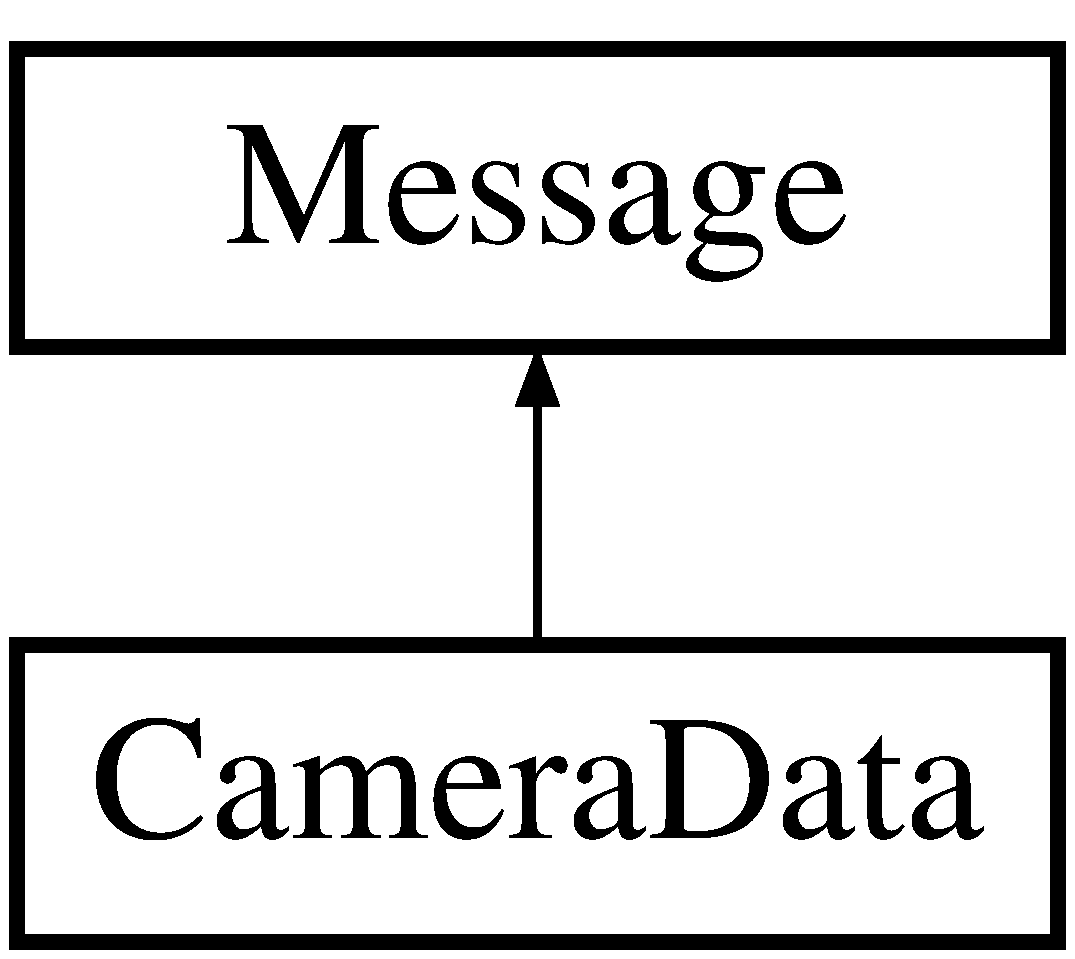
\includegraphics[height=2.000000cm]{classCameraData}
\end{center}
\end{figure}
\subsection*{Public Member Functions}
\begin{DoxyCompactItemize}
\item 
\hyperlink{classCameraData_af81f01ad4e2c27cc83e60c822bb1799d}{CameraData} (const QImage \&frame)
\item 
virtual \hyperlink{classCameraData_a480aa2bf05624b1530bc10f8ed80e977}{$\sim$CameraData} ()
\item 
const QImage \& \hyperlink{classCameraData_a6572495dbce01031c41587a91e0a73a1}{getFrame} () const 
\end{DoxyCompactItemize}


\subsection{Detailed Description}
Camera data message. 

This class contains a camera frame, signalled by \hyperlink{classCameraSensor}{CameraSensor}.

\begin{DoxySeeAlso}{See also}
\hyperlink{classCameraSensor}{CameraSensor} 
\end{DoxySeeAlso}


\subsection{Constructor \& Destructor Documentation}
\hypertarget{classCameraData_af81f01ad4e2c27cc83e60c822bb1799d}{
\index{CameraData@{CameraData}!CameraData@{CameraData}}
\index{CameraData@{CameraData}!CameraData@{CameraData}}
\subsubsection[{CameraData}]{\setlength{\rightskip}{0pt plus 5cm}CameraData::CameraData (
\begin{DoxyParamCaption}
\item[{const QImage \&}]{frame}
\end{DoxyParamCaption}
)}}
\label{classCameraData_af81f01ad4e2c27cc83e60c822bb1799d}
Constructs a new \hyperlink{classCameraData}{CameraData} message, containing a camera frame


\begin{DoxyParams}{Parameters}
{\em frame} & The camera frame \\
\hline
\end{DoxyParams}
\hypertarget{classCameraData_a480aa2bf05624b1530bc10f8ed80e977}{
\index{CameraData@{CameraData}!$\sim$CameraData@{$\sim$CameraData}}
\index{$\sim$CameraData@{$\sim$CameraData}!CameraData@{CameraData}}
\subsubsection[{$\sim$CameraData}]{\setlength{\rightskip}{0pt plus 5cm}CameraData::$\sim$CameraData (
\begin{DoxyParamCaption}
{}
\end{DoxyParamCaption}
)\hspace{0.3cm}{\ttfamily  \mbox{[}virtual\mbox{]}}}}
\label{classCameraData_a480aa2bf05624b1530bc10f8ed80e977}
Destroys the \hyperlink{classCameraData}{CameraData} 

\subsection{Member Function Documentation}
\hypertarget{classCameraData_a6572495dbce01031c41587a91e0a73a1}{
\index{CameraData@{CameraData}!getFrame@{getFrame}}
\index{getFrame@{getFrame}!CameraData@{CameraData}}
\subsubsection[{getFrame}]{\setlength{\rightskip}{0pt plus 5cm}const QImage \& CameraData::getFrame (
\begin{DoxyParamCaption}
{}
\end{DoxyParamCaption}
) const}}
\label{classCameraData_a6572495dbce01031c41587a91e0a73a1}
\begin{DoxyReturn}{Returns}
A const reference to the camera frame 
\end{DoxyReturn}


The documentation for this class was generated from the following files:\begin{DoxyCompactItemize}
\item 
data/\hyperlink{cameradata_8h}{cameradata.h}\item 
data/\hyperlink{cameradata_8cpp}{cameradata.cpp}\end{DoxyCompactItemize}

\hypertarget{classCameraSensor}{
\section{CameraSensor Class Reference}
\label{classCameraSensor}\index{CameraSensor@{CameraSensor}}
}


\hyperlink{classSensor}{Sensor} for camera data.  




{\ttfamily \#include $<$camerasensor.h$>$}

Inheritance diagram for CameraSensor:\begin{figure}[H]
\begin{center}
\leavevmode
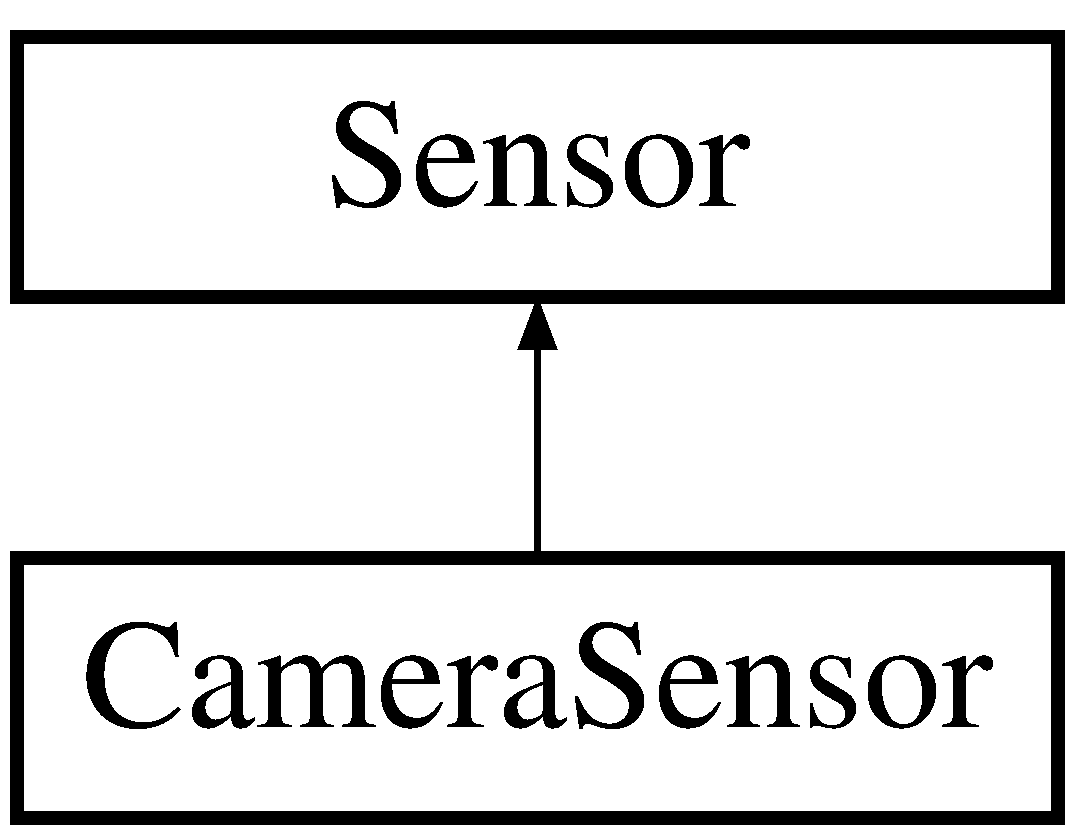
\includegraphics[height=2.000000cm]{classCameraSensor}
\end{center}
\end{figure}
\subsection*{Public Slots}
\begin{DoxyCompactItemize}
\item 
void \hyperlink{classCameraSensor_a7ac39be83c8f461b0d6e057d8b2d4011}{onMessageReceived} (const \hyperlink{classMessage}{Message} \&message)
\end{DoxyCompactItemize}
\subsection*{Public Member Functions}
\begin{DoxyCompactItemize}
\item 
\hyperlink{classCameraSensor_a0aed1ea5c345d9c964ec91ce35448e49}{CameraSensor} (QObject $\ast$parent=0)
\item 
virtual \hyperlink{classCameraSensor_ad55bb359dcb32fef636013e960e45a34}{$\sim$CameraSensor} ()
\end{DoxyCompactItemize}


\subsection{Detailed Description}
\hyperlink{classSensor}{Sensor} for camera data. 

\hyperlink{classCameraSensor}{CameraSensor} implements a \hyperlink{classSensor}{Sensor} that parses raw image data obtained by the UPIS controller and signals it through the common \hyperlink{classSensor}{Sensor} interface in the form of a \hyperlink{classCameraData}{CameraData} message

\begin{DoxySeeAlso}{See also}
\hyperlink{classCameraData}{CameraData} 
\end{DoxySeeAlso}


\subsection{Constructor \& Destructor Documentation}
\hypertarget{classCameraSensor_a0aed1ea5c345d9c964ec91ce35448e49}{
\index{CameraSensor@{CameraSensor}!CameraSensor@{CameraSensor}}
\index{CameraSensor@{CameraSensor}!CameraSensor@{CameraSensor}}
\subsubsection[{CameraSensor}]{\setlength{\rightskip}{0pt plus 5cm}CameraSensor::CameraSensor (
\begin{DoxyParamCaption}
\item[{QObject $\ast$}]{parent = {\ttfamily 0}}
\end{DoxyParamCaption}
)}}
\label{classCameraSensor_a0aed1ea5c345d9c964ec91ce35448e49}
Constructs a new \hyperlink{classCameraSensor}{CameraSensor}


\begin{DoxyParams}{Parameters}
{\em parent} & Optional QObject parent \\
\hline
\end{DoxyParams}
\hypertarget{classCameraSensor_ad55bb359dcb32fef636013e960e45a34}{
\index{CameraSensor@{CameraSensor}!$\sim$CameraSensor@{$\sim$CameraSensor}}
\index{$\sim$CameraSensor@{$\sim$CameraSensor}!CameraSensor@{CameraSensor}}
\subsubsection[{$\sim$CameraSensor}]{\setlength{\rightskip}{0pt plus 5cm}CameraSensor::$\sim$CameraSensor (
\begin{DoxyParamCaption}
{}
\end{DoxyParamCaption}
)\hspace{0.3cm}{\ttfamily  \mbox{[}virtual\mbox{]}}}}
\label{classCameraSensor_ad55bb359dcb32fef636013e960e45a34}
Destroys the \hyperlink{classCameraSensor}{CameraSensor} 

\subsection{Member Function Documentation}
\hypertarget{classCameraSensor_a7ac39be83c8f461b0d6e057d8b2d4011}{
\index{CameraSensor@{CameraSensor}!onMessageReceived@{onMessageReceived}}
\index{onMessageReceived@{onMessageReceived}!CameraSensor@{CameraSensor}}
\subsubsection[{onMessageReceived}]{\setlength{\rightskip}{0pt plus 5cm}void CameraSensor::onMessageReceived (
\begin{DoxyParamCaption}
\item[{const {\bf Message} \&}]{message}
\end{DoxyParamCaption}
)\hspace{0.3cm}{\ttfamily  \mbox{[}virtual, slot\mbox{]}}}}
\label{classCameraSensor_a7ac39be83c8f461b0d6e057d8b2d4011}
\hyperlink{classSensor_a71fbeb7fbebe8813ad74c57e45c066bc}{Sensor::onMessageReceived()} implementation for \hyperlink{classCameraSensor}{CameraSensor} 

Implements \hyperlink{classSensor_a71fbeb7fbebe8813ad74c57e45c066bc}{Sensor}.



The documentation for this class was generated from the following files:\begin{DoxyCompactItemize}
\item 
middleware/sensor/\hyperlink{camerasensor_8h}{camerasensor.h}\item 
middleware/sensor/\hyperlink{camerasensor_8cpp}{camerasensor.cpp}\end{DoxyCompactItemize}

\hypertarget{classDriver}{
\section{Driver Class Reference}
\label{classDriver}\index{Driver@{Driver}}
}


Generic driver interface.  




{\ttfamily \#include $<$driver.h$>$}

\subsection*{Public Slots}
\begin{DoxyCompactItemize}
\item 
virtual void \hyperlink{classDriver_af85a17da0276d26134cf02fb58063c38}{onDriverMessage} (const \hyperlink{classMessage}{Message} \&message)=0
\end{DoxyCompactItemize}
\subsection*{Signals}
\begin{DoxyCompactItemize}
\item 
void \hyperlink{classDriver_ae74285ffd8852815b1758950ccba7e96}{lowLevelCommand} (const \hyperlink{classMessage}{Message} \&data)
\end{DoxyCompactItemize}
\subsection*{Public Member Functions}
\begin{DoxyCompactItemize}
\item 
virtual \hyperlink{classDriver_ac7645eea8d3ce2bc39ddbda5e840297a}{$\sim$Driver} ()
\end{DoxyCompactItemize}
\subsection*{Protected Member Functions}
\begin{DoxyCompactItemize}
\item 
\hyperlink{classDriver_ad74d5b3e9b8f25e10f81d145a5fb316b}{Driver} (QObject $\ast$parent=0)
\end{DoxyCompactItemize}


\subsection{Detailed Description}
Generic driver interface. 

The \hyperlink{classSensor}{Sensor} virtual class defines the common interface that must be implemented by middleware classes that communicate commands to an underlying controller.

The particular command (\hyperlink{classMessage}{Message}) expected is dependent on the \hyperlink{classDriver}{Driver} implementation, hence additional information should be sought in the relative subclass documentation 

\subsection{Constructor \& Destructor Documentation}
\hypertarget{classDriver_ad74d5b3e9b8f25e10f81d145a5fb316b}{
\index{Driver@{Driver}!Driver@{Driver}}
\index{Driver@{Driver}!Driver@{Driver}}
\subsubsection[{Driver}]{\setlength{\rightskip}{0pt plus 5cm}Driver::Driver (
\begin{DoxyParamCaption}
\item[{QObject $\ast$}]{parent = {\ttfamily 0}}
\end{DoxyParamCaption}
)\hspace{0.3cm}{\ttfamily  \mbox{[}protected\mbox{]}}}}
\label{classDriver_ad74d5b3e9b8f25e10f81d145a5fb316b}
Constructs a new \hyperlink{classDriver}{Driver}


\begin{DoxyParams}{Parameters}
{\em parent} & Optional QObject parent \\
\hline
\end{DoxyParams}
\hypertarget{classDriver_ac7645eea8d3ce2bc39ddbda5e840297a}{
\index{Driver@{Driver}!$\sim$Driver@{$\sim$Driver}}
\index{$\sim$Driver@{$\sim$Driver}!Driver@{Driver}}
\subsubsection[{$\sim$Driver}]{\setlength{\rightskip}{0pt plus 5cm}Driver::$\sim$Driver (
\begin{DoxyParamCaption}
{}
\end{DoxyParamCaption}
)\hspace{0.3cm}{\ttfamily  \mbox{[}virtual\mbox{]}}}}
\label{classDriver_ac7645eea8d3ce2bc39ddbda5e840297a}
Destroys the \hyperlink{classDriver}{Driver} 

\subsection{Member Function Documentation}
\hypertarget{classDriver_ae74285ffd8852815b1758950ccba7e96}{
\index{Driver@{Driver}!lowLevelCommand@{lowLevelCommand}}
\index{lowLevelCommand@{lowLevelCommand}!Driver@{Driver}}
\subsubsection[{lowLevelCommand}]{\setlength{\rightskip}{0pt plus 5cm}void Driver::lowLevelCommand (
\begin{DoxyParamCaption}
\item[{const {\bf Message} \&}]{data}
\end{DoxyParamCaption}
)\hspace{0.3cm}{\ttfamily  \mbox{[}signal\mbox{]}}}}
\label{classDriver_ae74285ffd8852815b1758950ccba7e96}
This signal is emitted whenever the driver deems necessary to communicate a command to the underlying controller.


\begin{DoxyParams}{Parameters}
{\em data} & The command message aimed at the underlying controller \\
\hline
\end{DoxyParams}
\hypertarget{classDriver_af85a17da0276d26134cf02fb58063c38}{
\index{Driver@{Driver}!onDriverMessage@{onDriverMessage}}
\index{onDriverMessage@{onDriverMessage}!Driver@{Driver}}
\subsubsection[{onDriverMessage}]{\setlength{\rightskip}{0pt plus 5cm}virtual void Driver::onDriverMessage (
\begin{DoxyParamCaption}
\item[{const {\bf Message} \&}]{message}
\end{DoxyParamCaption}
)\hspace{0.3cm}{\ttfamily  \mbox{[}pure virtual, slot\mbox{]}}}}
\label{classDriver_af85a17da0276d26134cf02fb58063c38}
This slot must be implemented by subclasses in order to receive messages from the driver user (i.e. \hyperlink{classRobotController}{RobotController}). In case the message is of interest it should be interpreted and an appropriate lowLevelCommand signal should be emitted for the underlying controller.

Refer to the particular \hyperlink{classDriver}{Driver} implementation for information about the actual type of \hyperlink{classMessage}{Message} expected


\begin{DoxyParams}{Parameters}
{\em message} & The message sent by the driver user \\
\hline
\end{DoxyParams}


The documentation for this class was generated from the following files:\begin{DoxyCompactItemize}
\item 
middleware/driver/\hyperlink{driver_8h}{driver.h}\item 
middleware/driver/\hyperlink{driver_8cpp}{driver.cpp}\end{DoxyCompactItemize}

\hypertarget{classLaserData}{
\section{LaserData Class Reference}
\label{classLaserData}\index{LaserData@{LaserData}}
}


Laser data message.  




{\ttfamily \#include $<$laserdata.h$>$}

Inheritance diagram for LaserData:\begin{figure}[H]
\begin{center}
\leavevmode
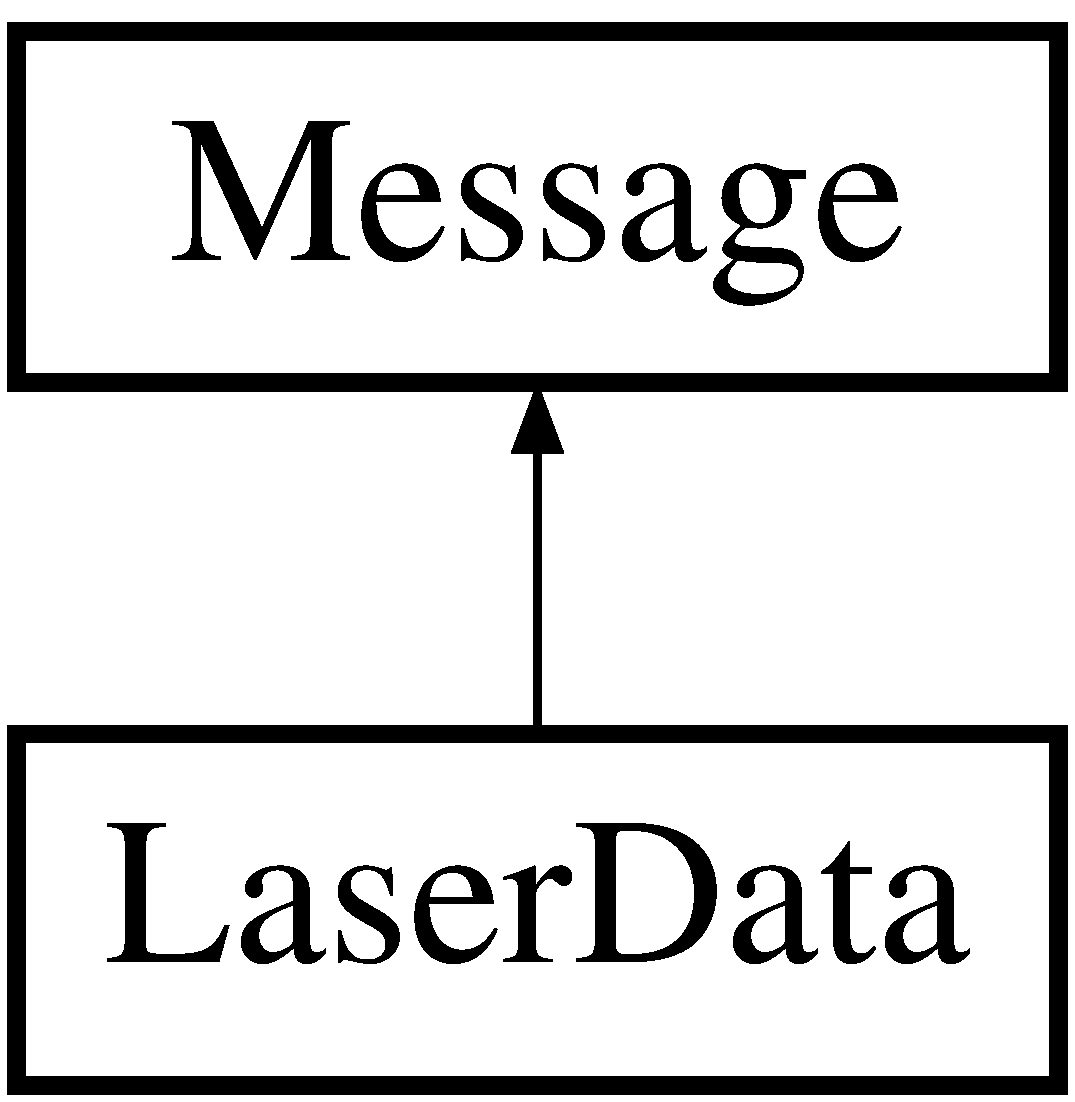
\includegraphics[height=2.000000cm]{classLaserData}
\end{center}
\end{figure}
\subsection*{Public Member Functions}
\begin{DoxyCompactItemize}
\item 
\hyperlink{classLaserData_aa774147523cb75f1a29a48ae9e966357}{LaserData} (double fov, double resolution, const QList$<$ double $>$ \&readings)
\item 
virtual \hyperlink{classLaserData_a4e3ebdad7df74033e606281b118874e8}{$\sim$LaserData} ()
\item 
const QList$<$ double $>$ \& \hyperlink{classLaserData_a21e8ace6cf591b71f174c54dff409886}{getReadings} () const 
\item 
double \hyperlink{classLaserData_a66ec4933e7529639fcdecf0d4c93088a}{getFOV} () const 
\item 
double \hyperlink{classLaserData_ae883461416b168cdc243cf1f03aedf1d}{getResolution} () const 
\end{DoxyCompactItemize}


\subsection{Detailed Description}
Laser data message. 

This class represents laser data readings, signalled by \hyperlink{classLaserSensor}{LaserSensor}

\begin{DoxySeeAlso}{See also}
\hyperlink{classLaserSensor}{LaserSensor} 
\end{DoxySeeAlso}


\subsection{Constructor \& Destructor Documentation}
\hypertarget{classLaserData_aa774147523cb75f1a29a48ae9e966357}{
\index{LaserData@{LaserData}!LaserData@{LaserData}}
\index{LaserData@{LaserData}!LaserData@{LaserData}}
\subsubsection[{LaserData}]{\setlength{\rightskip}{0pt plus 5cm}LaserData::LaserData (
\begin{DoxyParamCaption}
\item[{double}]{fov, }
\item[{double}]{resolution, }
\item[{const QList$<$ double $>$ \&}]{readings}
\end{DoxyParamCaption}
)}}
\label{classLaserData_aa774147523cb75f1a29a48ae9e966357}
Constructs a new \hyperlink{classLaserData}{LaserData} message, containing the readings and properties of the laser sensor


\begin{DoxyParams}{Parameters}
{\em fov} & The field of view of the laser sensor \\
\hline
{\em resolution} & The tick resolution of the laser sensor (in radiants) \\
\hline
{\em readings} & The list of dinstance readings \\
\hline
\end{DoxyParams}
\hypertarget{classLaserData_a4e3ebdad7df74033e606281b118874e8}{
\index{LaserData@{LaserData}!$\sim$LaserData@{$\sim$LaserData}}
\index{$\sim$LaserData@{$\sim$LaserData}!LaserData@{LaserData}}
\subsubsection[{$\sim$LaserData}]{\setlength{\rightskip}{0pt plus 5cm}LaserData::$\sim$LaserData (
\begin{DoxyParamCaption}
{}
\end{DoxyParamCaption}
)\hspace{0.3cm}{\ttfamily  \mbox{[}virtual\mbox{]}}}}
\label{classLaserData_a4e3ebdad7df74033e606281b118874e8}
Destroys the \hyperlink{classLaserData}{LaserData} 

\subsection{Member Function Documentation}
\hypertarget{classLaserData_a66ec4933e7529639fcdecf0d4c93088a}{
\index{LaserData@{LaserData}!getFOV@{getFOV}}
\index{getFOV@{getFOV}!LaserData@{LaserData}}
\subsubsection[{getFOV}]{\setlength{\rightskip}{0pt plus 5cm}double LaserData::getFOV (
\begin{DoxyParamCaption}
{}
\end{DoxyParamCaption}
) const}}
\label{classLaserData_a66ec4933e7529639fcdecf0d4c93088a}
\begin{DoxyReturn}{Returns}
The field of view of the laser sensor 
\end{DoxyReturn}
\hypertarget{classLaserData_a21e8ace6cf591b71f174c54dff409886}{
\index{LaserData@{LaserData}!getReadings@{getReadings}}
\index{getReadings@{getReadings}!LaserData@{LaserData}}
\subsubsection[{getReadings}]{\setlength{\rightskip}{0pt plus 5cm}const QList$<$ double $>$ \& LaserData::getReadings (
\begin{DoxyParamCaption}
{}
\end{DoxyParamCaption}
) const}}
\label{classLaserData_a21e8ace6cf591b71f174c54dff409886}
\begin{DoxyReturn}{Returns}
A const reference to the list of distance readings 
\end{DoxyReturn}
\hypertarget{classLaserData_ae883461416b168cdc243cf1f03aedf1d}{
\index{LaserData@{LaserData}!getResolution@{getResolution}}
\index{getResolution@{getResolution}!LaserData@{LaserData}}
\subsubsection[{getResolution}]{\setlength{\rightskip}{0pt plus 5cm}double LaserData::getResolution (
\begin{DoxyParamCaption}
{}
\end{DoxyParamCaption}
) const}}
\label{classLaserData_ae883461416b168cdc243cf1f03aedf1d}
\begin{DoxyReturn}{Returns}
The tick resolution of the laser sensor (in radiants) 
\end{DoxyReturn}


The documentation for this class was generated from the following files:\begin{DoxyCompactItemize}
\item 
data/\hyperlink{laserdata_8h}{laserdata.h}\item 
data/\hyperlink{laserdata_8cpp}{laserdata.cpp}\end{DoxyCompactItemize}

\hypertarget{classLaserSensor}{
\section{LaserSensor Class Reference}
\label{classLaserSensor}\index{LaserSensor@{LaserSensor}}
}


\hyperlink{classSensor}{Sensor} for laser scans.  




{\ttfamily \#include $<$lasersensor.h$>$}

Inheritance diagram for LaserSensor:\begin{figure}[H]
\begin{center}
\leavevmode
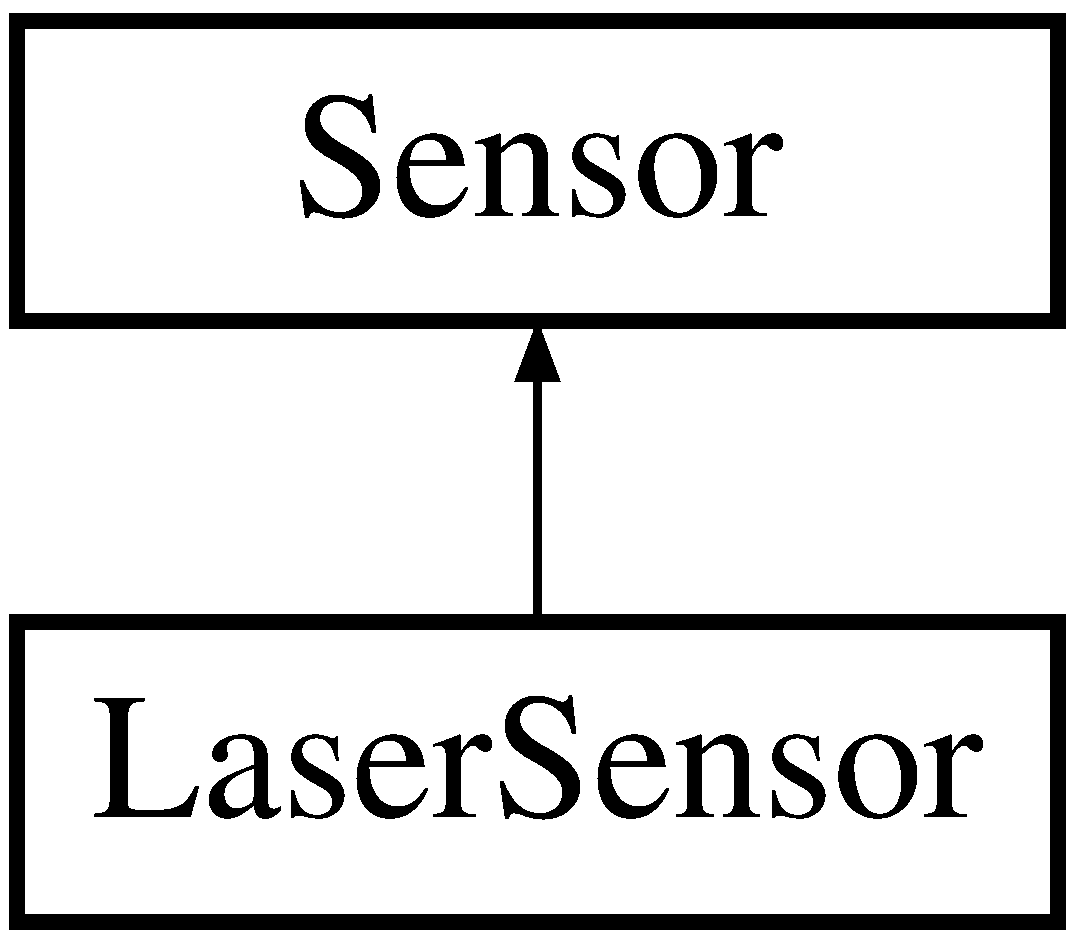
\includegraphics[height=2.000000cm]{classLaserSensor}
\end{center}
\end{figure}
\subsection*{Public Slots}
\begin{DoxyCompactItemize}
\item 
virtual void \hyperlink{classLaserSensor_aa7b966f0849ce5c43920480abcae50f0}{onMessageReceived} (const \hyperlink{classMessage}{Message} \&message)
\end{DoxyCompactItemize}
\subsection*{Public Member Functions}
\begin{DoxyCompactItemize}
\item 
\hyperlink{classLaserSensor_a342c1557c4dbfa0401efa0c50dc0c6fb}{LaserSensor} (QObject $\ast$parent=0)
\item 
virtual \hyperlink{classLaserSensor_a3a1c45b4a6206163c713dbeec1d5d735}{$\sim$LaserSensor} ()
\end{DoxyCompactItemize}


\subsection{Detailed Description}
\hyperlink{classSensor}{Sensor} for laser scans. 

\hyperlink{classLaserSensor}{LaserSensor} implements a \hyperlink{classSensor}{Sensor} that parses laser data and signals it through the common \hyperlink{classSensor}{Sensor} interface in the form of \hyperlink{classLaserData}{LaserData} message

\begin{DoxySeeAlso}{See also}
\hyperlink{classLaserData}{LaserData} 
\end{DoxySeeAlso}


\subsection{Constructor \& Destructor Documentation}
\hypertarget{classLaserSensor_a342c1557c4dbfa0401efa0c50dc0c6fb}{
\index{LaserSensor@{LaserSensor}!LaserSensor@{LaserSensor}}
\index{LaserSensor@{LaserSensor}!LaserSensor@{LaserSensor}}
\subsubsection[{LaserSensor}]{\setlength{\rightskip}{0pt plus 5cm}LaserSensor::LaserSensor (
\begin{DoxyParamCaption}
\item[{QObject $\ast$}]{parent = {\ttfamily 0}}
\end{DoxyParamCaption}
)}}
\label{classLaserSensor_a342c1557c4dbfa0401efa0c50dc0c6fb}
Constructs a new \hyperlink{classLaserSensor}{LaserSensor}


\begin{DoxyParams}{Parameters}
{\em parent} & Optional QObject parent \\
\hline
\end{DoxyParams}
\hypertarget{classLaserSensor_a3a1c45b4a6206163c713dbeec1d5d735}{
\index{LaserSensor@{LaserSensor}!$\sim$LaserSensor@{$\sim$LaserSensor}}
\index{$\sim$LaserSensor@{$\sim$LaserSensor}!LaserSensor@{LaserSensor}}
\subsubsection[{$\sim$LaserSensor}]{\setlength{\rightskip}{0pt plus 5cm}LaserSensor::$\sim$LaserSensor (
\begin{DoxyParamCaption}
{}
\end{DoxyParamCaption}
)\hspace{0.3cm}{\ttfamily  \mbox{[}virtual\mbox{]}}}}
\label{classLaserSensor_a3a1c45b4a6206163c713dbeec1d5d735}
Destroys the \hyperlink{classLaserSensor}{LaserSensor} 

\subsection{Member Function Documentation}
\hypertarget{classLaserSensor_aa7b966f0849ce5c43920480abcae50f0}{
\index{LaserSensor@{LaserSensor}!onMessageReceived@{onMessageReceived}}
\index{onMessageReceived@{onMessageReceived}!LaserSensor@{LaserSensor}}
\subsubsection[{onMessageReceived}]{\setlength{\rightskip}{0pt plus 5cm}void LaserSensor::onMessageReceived (
\begin{DoxyParamCaption}
\item[{const {\bf Message} \&}]{message}
\end{DoxyParamCaption}
)\hspace{0.3cm}{\ttfamily  \mbox{[}virtual, slot\mbox{]}}}}
\label{classLaserSensor_aa7b966f0849ce5c43920480abcae50f0}
\hyperlink{classSensor_a71fbeb7fbebe8813ad74c57e45c066bc}{Sensor::onMessageReceived()} implementation for \hyperlink{classLaserSensor}{LaserSensor} 

Implements \hyperlink{classSensor_a71fbeb7fbebe8813ad74c57e45c066bc}{Sensor}.



The documentation for this class was generated from the following files:\begin{DoxyCompactItemize}
\item 
middleware/sensor/\hyperlink{lasersensor_8h}{lasersensor.h}\item 
middleware/sensor/\hyperlink{lasersensor_8cpp}{lasersensor.cpp}\end{DoxyCompactItemize}

\hypertarget{classMessage}{
\section{Message Class Reference}
\label{classMessage}\index{Message@{Message}}
}


Generic message container.  




{\ttfamily \#include $<$message.h$>$}

Inheritance diagram for Message:\begin{figure}[H]
\begin{center}
\leavevmode
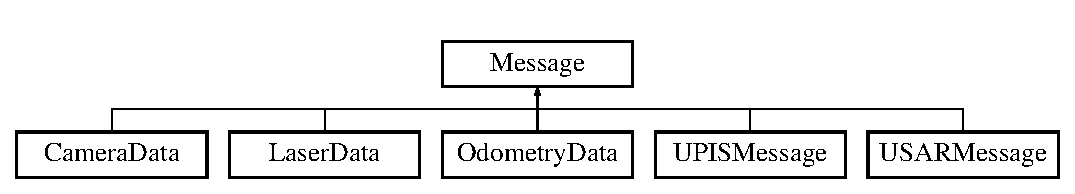
\includegraphics[height=2.000000cm]{classMessage}
\end{center}
\end{figure}
\subsection*{Public Member Functions}
\begin{DoxyCompactItemize}
\item 
virtual \hyperlink{classMessage_a58bb4122c52eaf1ac8f68d3ea0f151b8}{operator QString} ()
\end{DoxyCompactItemize}


\subsection{Detailed Description}
Generic message container. 

The \hyperlink{classMessage}{Message} class represents a common interface for message exchange used for sensors, drivers, low-\/level controllers and so on

\begin{DoxySeeAlso}{See also}
\hyperlink{classSensor}{Sensor} 

\hyperlink{classDriver}{Driver} 
\end{DoxySeeAlso}


\subsection{Member Function Documentation}
\hypertarget{classMessage_a58bb4122c52eaf1ac8f68d3ea0f151b8}{
\index{Message@{Message}!operator QString@{operator QString}}
\index{operator QString@{operator QString}!Message@{Message}}
\subsubsection[{operator QString}]{\setlength{\rightskip}{0pt plus 5cm}virtual Message::operator QString (
\begin{DoxyParamCaption}
{}
\end{DoxyParamCaption}
)\hspace{0.3cm}{\ttfamily  \mbox{[}inline, virtual\mbox{]}}}}
\label{classMessage_a58bb4122c52eaf1ac8f68d3ea0f151b8}
This method is meant to be overridden by subclasses, it provides a string representation of the \hyperlink{classMessage}{Message} (or just some information about it). A default empty string implementation is provided. The presence of this virtual method also ensures that RTTI support is compiled in for this class

\begin{DoxyReturn}{Returns}
A string representation of the \hyperlink{classMessage}{Message} 
\end{DoxyReturn}


The documentation for this class was generated from the following file:\begin{DoxyCompactItemize}
\item 
data/\hyperlink{message_8h}{message.h}\end{DoxyCompactItemize}

\hypertarget{classOdometryData}{
\section{OdometryData Class Reference}
\label{classOdometryData}\index{OdometryData@{OdometryData}}
}


Odometric data message.  




{\ttfamily \#include $<$odometrydata.h$>$}

Inheritance diagram for OdometryData:\begin{figure}[H]
\begin{center}
\leavevmode
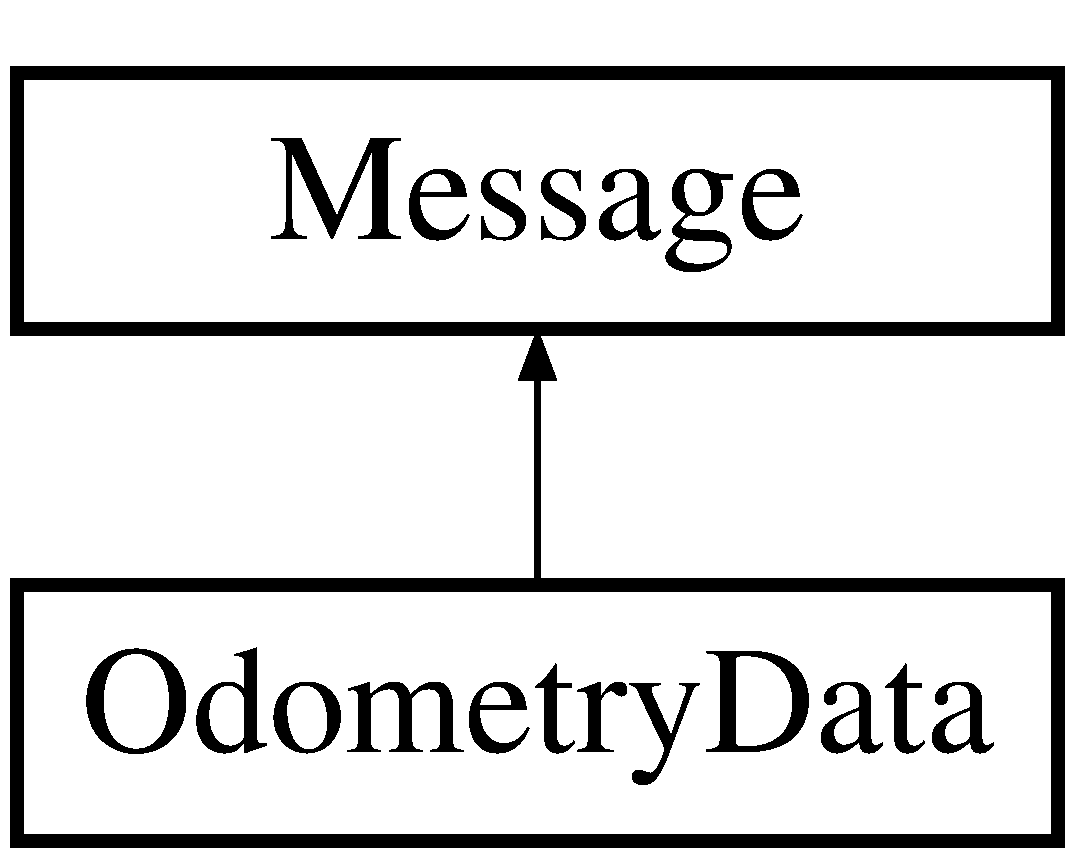
\includegraphics[height=2.000000cm]{classOdometryData}
\end{center}
\end{figure}
\subsection*{Public Member Functions}
\begin{DoxyCompactItemize}
\item 
\hyperlink{classOdometryData_a90766d087ca7e268ef563397f87d4f20}{OdometryData} (const \hyperlink{classPose}{Pose} \&pose)
\item 
virtual \hyperlink{classOdometryData_a0f76667e8bc97dfa401b25269233b6e8}{$\sim$OdometryData} ()
\item 
const \hyperlink{classPose}{Pose} \& \hyperlink{classOdometryData_ae8e1a74393a3608595a35ca14bf3eaaa}{getPose} () const 
\end{DoxyCompactItemize}


\subsection{Detailed Description}
Odometric data message. 

This class represents odometric data readings, signalled by \hyperlink{classOdometrySensor}{OdometrySensor}

\begin{DoxySeeAlso}{See also}
\hyperlink{classOdometrySensor}{OdometrySensor} 
\end{DoxySeeAlso}


\subsection{Constructor \& Destructor Documentation}
\hypertarget{classOdometryData_a90766d087ca7e268ef563397f87d4f20}{
\index{OdometryData@{OdometryData}!OdometryData@{OdometryData}}
\index{OdometryData@{OdometryData}!OdometryData@{OdometryData}}
\subsubsection[{OdometryData}]{\setlength{\rightskip}{0pt plus 5cm}OdometryData::OdometryData (
\begin{DoxyParamCaption}
\item[{const {\bf Pose} \&}]{pose}
\end{DoxyParamCaption}
)}}
\label{classOdometryData_a90766d087ca7e268ef563397f87d4f20}
Constructs a new \hyperlink{classOdometryData}{OdometryData} message


\begin{DoxyParams}{Parameters}
{\em pose} & The pose as reported by the odometric sensor \\
\hline
\end{DoxyParams}
\hypertarget{classOdometryData_a0f76667e8bc97dfa401b25269233b6e8}{
\index{OdometryData@{OdometryData}!$\sim$OdometryData@{$\sim$OdometryData}}
\index{$\sim$OdometryData@{$\sim$OdometryData}!OdometryData@{OdometryData}}
\subsubsection[{$\sim$OdometryData}]{\setlength{\rightskip}{0pt plus 5cm}OdometryData::$\sim$OdometryData (
\begin{DoxyParamCaption}
{}
\end{DoxyParamCaption}
)\hspace{0.3cm}{\ttfamily  \mbox{[}virtual\mbox{]}}}}
\label{classOdometryData_a0f76667e8bc97dfa401b25269233b6e8}
Destroys the \hyperlink{classOdometryData}{OdometryData} 

\subsection{Member Function Documentation}
\hypertarget{classOdometryData_ae8e1a74393a3608595a35ca14bf3eaaa}{
\index{OdometryData@{OdometryData}!getPose@{getPose}}
\index{getPose@{getPose}!OdometryData@{OdometryData}}
\subsubsection[{getPose}]{\setlength{\rightskip}{0pt plus 5cm}const {\bf Pose} \& OdometryData::getPose (
\begin{DoxyParamCaption}
{}
\end{DoxyParamCaption}
) const}}
\label{classOdometryData_ae8e1a74393a3608595a35ca14bf3eaaa}
\begin{DoxyReturn}{Returns}
The pose as reported by the odometric sensor 
\end{DoxyReturn}


The documentation for this class was generated from the following files:\begin{DoxyCompactItemize}
\item 
data/\hyperlink{odometrydata_8h}{odometrydata.h}\item 
data/\hyperlink{odometrydata_8cpp}{odometrydata.cpp}\end{DoxyCompactItemize}

\hypertarget{classOdometrySensor}{
\section{OdometrySensor Class Reference}
\label{classOdometrySensor}\index{OdometrySensor@{OdometrySensor}}
}


\hyperlink{classSensor}{Sensor} for odometric data.  




{\ttfamily \#include $<$odometrysensor.h$>$}

Inheritance diagram for OdometrySensor:\begin{figure}[H]
\begin{center}
\leavevmode
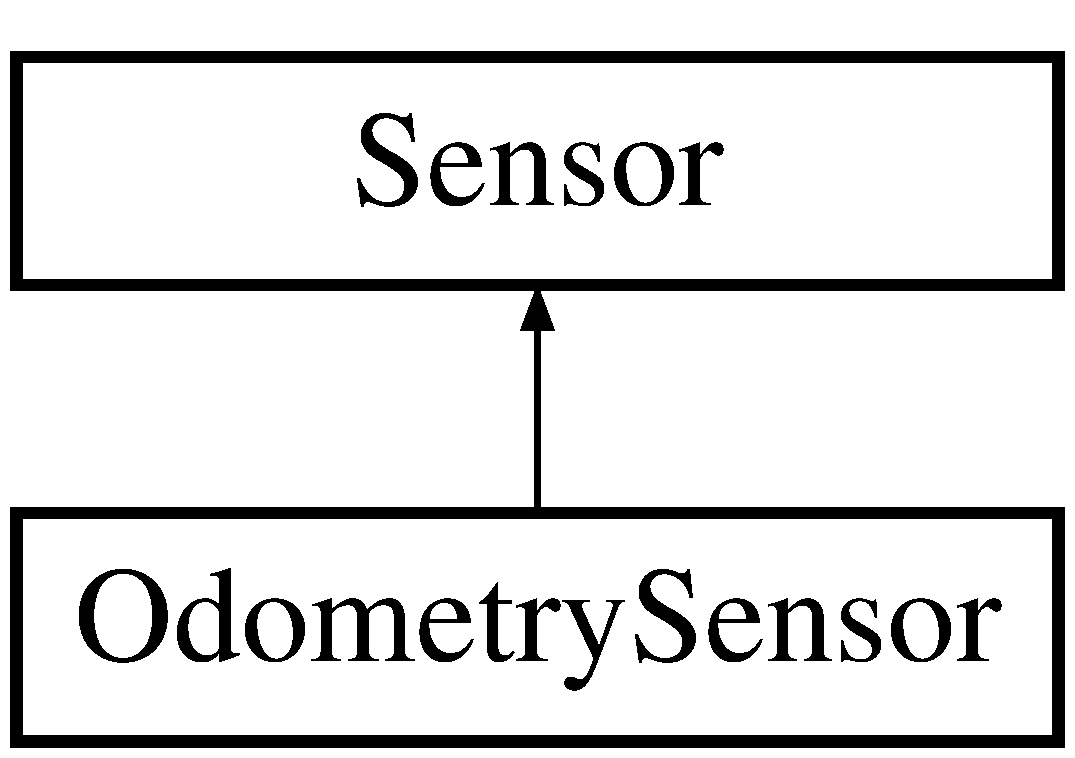
\includegraphics[height=2.000000cm]{classOdometrySensor}
\end{center}
\end{figure}
\subsection*{Public Slots}
\begin{DoxyCompactItemize}
\item 
virtual void \hyperlink{classOdometrySensor_a31000cc77d015a52c4b9d43996ed6ae8}{onMessageReceived} (const \hyperlink{classMessage}{Message} \&message)
\end{DoxyCompactItemize}
\subsection*{Public Member Functions}
\begin{DoxyCompactItemize}
\item 
\hyperlink{classOdometrySensor_a437a9b96f46dd58fc93355404cdff683}{OdometrySensor} (QObject $\ast$parent=0)
\item 
virtual \hyperlink{classOdometrySensor_a6ad98746685f391390ae75f252c609e2}{$\sim$OdometrySensor} ()
\end{DoxyCompactItemize}


\subsection{Detailed Description}
\hyperlink{classSensor}{Sensor} for odometric data. 

\hyperlink{classOdometrySensor}{OdometrySensor} implements a \hyperlink{classSensor}{Sensor} that parses odometric data and signals it through the common \hyperlink{classSensor}{Sensor} interface in the form of an \hyperlink{classOdometryData}{OdometryData} message

\begin{DoxySeeAlso}{See also}
\hyperlink{classOdometryData}{OdometryData} 
\end{DoxySeeAlso}


\subsection{Constructor \& Destructor Documentation}
\hypertarget{classOdometrySensor_a437a9b96f46dd58fc93355404cdff683}{
\index{OdometrySensor@{OdometrySensor}!OdometrySensor@{OdometrySensor}}
\index{OdometrySensor@{OdometrySensor}!OdometrySensor@{OdometrySensor}}
\subsubsection[{OdometrySensor}]{\setlength{\rightskip}{0pt plus 5cm}OdometrySensor::OdometrySensor (
\begin{DoxyParamCaption}
\item[{QObject $\ast$}]{parent = {\ttfamily 0}}
\end{DoxyParamCaption}
)}}
\label{classOdometrySensor_a437a9b96f46dd58fc93355404cdff683}
Constructs a new \hyperlink{classOdometrySensor}{OdometrySensor}


\begin{DoxyParams}{Parameters}
{\em parent} & Optional QObject parent \\
\hline
\end{DoxyParams}
\hypertarget{classOdometrySensor_a6ad98746685f391390ae75f252c609e2}{
\index{OdometrySensor@{OdometrySensor}!$\sim$OdometrySensor@{$\sim$OdometrySensor}}
\index{$\sim$OdometrySensor@{$\sim$OdometrySensor}!OdometrySensor@{OdometrySensor}}
\subsubsection[{$\sim$OdometrySensor}]{\setlength{\rightskip}{0pt plus 5cm}OdometrySensor::$\sim$OdometrySensor (
\begin{DoxyParamCaption}
{}
\end{DoxyParamCaption}
)\hspace{0.3cm}{\ttfamily  \mbox{[}virtual\mbox{]}}}}
\label{classOdometrySensor_a6ad98746685f391390ae75f252c609e2}
Destroys the \hyperlink{classOdometrySensor}{OdometrySensor} 

\subsection{Member Function Documentation}
\hypertarget{classOdometrySensor_a31000cc77d015a52c4b9d43996ed6ae8}{
\index{OdometrySensor@{OdometrySensor}!onMessageReceived@{onMessageReceived}}
\index{onMessageReceived@{onMessageReceived}!OdometrySensor@{OdometrySensor}}
\subsubsection[{onMessageReceived}]{\setlength{\rightskip}{0pt plus 5cm}void OdometrySensor::onMessageReceived (
\begin{DoxyParamCaption}
\item[{const {\bf Message} \&}]{message}
\end{DoxyParamCaption}
)\hspace{0.3cm}{\ttfamily  \mbox{[}virtual, slot\mbox{]}}}}
\label{classOdometrySensor_a31000cc77d015a52c4b9d43996ed6ae8}
\hyperlink{classSensor_a71fbeb7fbebe8813ad74c57e45c066bc}{Sensor::onMessageReceived()} implementation for \hyperlink{classOdometrySensor}{OdometrySensor} 

Implements \hyperlink{classSensor_a71fbeb7fbebe8813ad74c57e45c066bc}{Sensor}.



The documentation for this class was generated from the following files:\begin{DoxyCompactItemize}
\item 
middleware/sensor/\hyperlink{odometrysensor_8h}{odometrysensor.h}\item 
middleware/sensor/\hyperlink{odometrysensor_8cpp}{odometrysensor.cpp}\end{DoxyCompactItemize}

\hypertarget{classPose}{
\section{Pose Class Reference}
\label{classPose}\index{Pose@{Pose}}
}


{\ttfamily \#include $<$pose.h$>$}

\subsection*{Public Member Functions}
\begin{DoxyCompactItemize}
\item 
\hyperlink{classPose_a3190874545bf1b5c34d2b9d777a0c57a}{Pose} (double aX, double aY, double aTheta)
\item 
\hyperlink{classPose_a855e906f2cea943121e4dad4ef6a68d0}{Pose} (const \hyperlink{classPose}{Pose} \&aPose)
\item 
virtual \hyperlink{classPose_a4267a4b362912dded8377f2c3260803e}{$\sim$Pose} ()
\item 
double \hyperlink{classPose_a7beb15c5b0438d293be8ec3d4c3f2fdf}{getX} () const 
\item 
double \hyperlink{classPose_a0b9bdaa51e619192b9a2c887a4cd96d1}{getY} () const 
\item 
double \hyperlink{classPose_ad4462d069a56f658dcbeb8bcd3250979}{getTheta} () const 
\item 
void \hyperlink{classPose_ad43f05063999f3394127759c80b444cf}{setX} (double aX)
\item 
void \hyperlink{classPose_af29d6c361e7c0f3fb6848653dfc195c9}{setY} (double aY)
\item 
void \hyperlink{classPose_a83c2f037c4dbf55708ac298b54e5ee17}{setTheta} (double aTheta)
\end{DoxyCompactItemize}


\subsection{Constructor \& Destructor Documentation}
\hypertarget{classPose_a3190874545bf1b5c34d2b9d777a0c57a}{
\index{Pose@{Pose}!Pose@{Pose}}
\index{Pose@{Pose}!Pose@{Pose}}
\subsubsection[{Pose}]{\setlength{\rightskip}{0pt plus 5cm}Pose::Pose (
\begin{DoxyParamCaption}
\item[{double}]{aX, }
\item[{double}]{aY, }
\item[{double}]{aTheta}
\end{DoxyParamCaption}
)}}
\label{classPose_a3190874545bf1b5c34d2b9d777a0c57a}
\hypertarget{classPose_a855e906f2cea943121e4dad4ef6a68d0}{
\index{Pose@{Pose}!Pose@{Pose}}
\index{Pose@{Pose}!Pose@{Pose}}
\subsubsection[{Pose}]{\setlength{\rightskip}{0pt plus 5cm}Pose::Pose (
\begin{DoxyParamCaption}
\item[{const {\bf Pose} \&}]{aPose}
\end{DoxyParamCaption}
)}}
\label{classPose_a855e906f2cea943121e4dad4ef6a68d0}
\hypertarget{classPose_a4267a4b362912dded8377f2c3260803e}{
\index{Pose@{Pose}!$\sim$Pose@{$\sim$Pose}}
\index{$\sim$Pose@{$\sim$Pose}!Pose@{Pose}}
\subsubsection[{$\sim$Pose}]{\setlength{\rightskip}{0pt plus 5cm}Pose::$\sim$Pose (
\begin{DoxyParamCaption}
{}
\end{DoxyParamCaption}
)\hspace{0.3cm}{\ttfamily  \mbox{[}virtual\mbox{]}}}}
\label{classPose_a4267a4b362912dded8377f2c3260803e}


\subsection{Member Function Documentation}
\hypertarget{classPose_ad4462d069a56f658dcbeb8bcd3250979}{
\index{Pose@{Pose}!getTheta@{getTheta}}
\index{getTheta@{getTheta}!Pose@{Pose}}
\subsubsection[{getTheta}]{\setlength{\rightskip}{0pt plus 5cm}double Pose::getTheta (
\begin{DoxyParamCaption}
{}
\end{DoxyParamCaption}
) const}}
\label{classPose_ad4462d069a56f658dcbeb8bcd3250979}
\hypertarget{classPose_a7beb15c5b0438d293be8ec3d4c3f2fdf}{
\index{Pose@{Pose}!getX@{getX}}
\index{getX@{getX}!Pose@{Pose}}
\subsubsection[{getX}]{\setlength{\rightskip}{0pt plus 5cm}double Pose::getX (
\begin{DoxyParamCaption}
{}
\end{DoxyParamCaption}
) const}}
\label{classPose_a7beb15c5b0438d293be8ec3d4c3f2fdf}
\hypertarget{classPose_a0b9bdaa51e619192b9a2c887a4cd96d1}{
\index{Pose@{Pose}!getY@{getY}}
\index{getY@{getY}!Pose@{Pose}}
\subsubsection[{getY}]{\setlength{\rightskip}{0pt plus 5cm}double Pose::getY (
\begin{DoxyParamCaption}
{}
\end{DoxyParamCaption}
) const}}
\label{classPose_a0b9bdaa51e619192b9a2c887a4cd96d1}
\hypertarget{classPose_a83c2f037c4dbf55708ac298b54e5ee17}{
\index{Pose@{Pose}!setTheta@{setTheta}}
\index{setTheta@{setTheta}!Pose@{Pose}}
\subsubsection[{setTheta}]{\setlength{\rightskip}{0pt plus 5cm}void Pose::setTheta (
\begin{DoxyParamCaption}
\item[{double}]{aTheta}
\end{DoxyParamCaption}
)}}
\label{classPose_a83c2f037c4dbf55708ac298b54e5ee17}
\hypertarget{classPose_ad43f05063999f3394127759c80b444cf}{
\index{Pose@{Pose}!setX@{setX}}
\index{setX@{setX}!Pose@{Pose}}
\subsubsection[{setX}]{\setlength{\rightskip}{0pt plus 5cm}void Pose::setX (
\begin{DoxyParamCaption}
\item[{double}]{aX}
\end{DoxyParamCaption}
)}}
\label{classPose_ad43f05063999f3394127759c80b444cf}
\hypertarget{classPose_af29d6c361e7c0f3fb6848653dfc195c9}{
\index{Pose@{Pose}!setY@{setY}}
\index{setY@{setY}!Pose@{Pose}}
\subsubsection[{setY}]{\setlength{\rightskip}{0pt plus 5cm}void Pose::setY (
\begin{DoxyParamCaption}
\item[{double}]{aY}
\end{DoxyParamCaption}
)}}
\label{classPose_af29d6c361e7c0f3fb6848653dfc195c9}


The documentation for this class was generated from the following files:\begin{DoxyCompactItemize}
\item 
data/\hyperlink{pose_8h}{pose.h}\item 
data/\hyperlink{pose_8cpp}{pose.cpp}\end{DoxyCompactItemize}

\hypertarget{classRobot}{
\section{Robot Class Reference}
\label{classRobot}\index{Robot@{Robot}}
}


{\ttfamily \#include $<$robot.h$>$}

\subsection*{Public Member Functions}
\begin{DoxyCompactItemize}
\item 
\hyperlink{classRobot_a0f2108bd63b096f1b55fee82f7366895}{Robot} (const QString \&location, const uint identifier, QObject $\ast$parent=0)
\item 
virtual \hyperlink{classRobot_a924320124b09c2f2ac1621aa210d5f38}{$\sim$Robot} ()
\item 
void \hyperlink{classRobot_aba6fa8d5cbf173ca0df078c6212612fd}{spawnRobot} (const QString \&usarAddress, const quint16 usarPort, const QString \&upisAddress, const quint16 upisPort)
\end{DoxyCompactItemize}


\subsection{Detailed Description}
This class represents the high-\/level robot. It connects the sensors and the drivers to the controllers that are connected to the servers 

\subsection{Constructor \& Destructor Documentation}
\hypertarget{classRobot_a0f2108bd63b096f1b55fee82f7366895}{
\index{Robot@{Robot}!Robot@{Robot}}
\index{Robot@{Robot}!Robot@{Robot}}
\subsubsection[{Robot}]{\setlength{\rightskip}{0pt plus 5cm}Robot::Robot (
\begin{DoxyParamCaption}
\item[{const QString \&}]{location, }
\item[{const uint}]{identifier, }
\item[{QObject $\ast$}]{parent = {\ttfamily 0}}
\end{DoxyParamCaption}
)\hspace{0.3cm}{\ttfamily  \mbox{[}explicit\mbox{]}}}}
\label{classRobot_a0f2108bd63b096f1b55fee82f7366895}
Contructor for the robot. \hypertarget{classRobot_a924320124b09c2f2ac1621aa210d5f38}{
\index{Robot@{Robot}!$\sim$Robot@{$\sim$Robot}}
\index{$\sim$Robot@{$\sim$Robot}!Robot@{Robot}}
\subsubsection[{$\sim$Robot}]{\setlength{\rightskip}{0pt plus 5cm}Robot::$\sim$Robot (
\begin{DoxyParamCaption}
{}
\end{DoxyParamCaption}
)\hspace{0.3cm}{\ttfamily  \mbox{[}virtual\mbox{]}}}}
\label{classRobot_a924320124b09c2f2ac1621aa210d5f38}
Destructor for the robot. 

\subsection{Member Function Documentation}
\hypertarget{classRobot_aba6fa8d5cbf173ca0df078c6212612fd}{
\index{Robot@{Robot}!spawnRobot@{spawnRobot}}
\index{spawnRobot@{spawnRobot}!Robot@{Robot}}
\subsubsection[{spawnRobot}]{\setlength{\rightskip}{0pt plus 5cm}void Robot::spawnRobot (
\begin{DoxyParamCaption}
\item[{const QString \&}]{usarAddress, }
\item[{const quint16}]{usarPort, }
\item[{const QString \&}]{upisAddress, }
\item[{const quint16}]{upisPort}
\end{DoxyParamCaption}
)}}
\label{classRobot_aba6fa8d5cbf173ca0df078c6212612fd}
Method that spawns a robot in the simulation, connecting it to USARSim and to UPIS. 
\begin{DoxyParams}{Parameters}
{\em usarAddress} & the IP address of USARSim. \\
\hline
{\em usarPort} & the port of USARSim. \\
\hline
{\em upisAddress} & the IP address of UPIS. \\
\hline
{\em upisPort} & the port of UPIS. \\
\hline
\end{DoxyParams}


The documentation for this class was generated from the following files:\begin{DoxyCompactItemize}
\item 
logic/\hyperlink{robot_8h}{robot.h}\item 
logic/\hyperlink{robot_8cpp}{robot.cpp}\end{DoxyCompactItemize}

\hypertarget{classRobotController}{
\section{RobotController Class Reference}
\label{classRobotController}\index{RobotController@{RobotController}}
}


{\ttfamily \#include $<$robotcontroller.h$>$}

\subsection*{Public Slots}
\begin{DoxyCompactItemize}
\item 
void \hyperlink{classRobotController_af7a4ba9ea79c8905b428b2bf1b7e2c5b}{onStateUpdated} ()
\item 
void \hyperlink{classRobotController_a9493a7011af6b4b31413ed42fe3fc518}{onSensorData} (const \hyperlink{classMessage}{Message} \&data)
\end{DoxyCompactItemize}
\subsection*{Signals}
\begin{DoxyCompactItemize}
\item 
void \hyperlink{classRobotController_a4c89049efc91e8d172dc9ca6a78f50fd}{launchCommand} (const QString \&command)
\item 
void \hyperlink{classRobotController_acf08e56717b3134fee7e36f481746e8f}{stateUpdate} ()
\end{DoxyCompactItemize}
\subsection*{Public Member Functions}
\begin{DoxyCompactItemize}
\item 
\hyperlink{classRobotController_af0d6c5568c619b1931792d1fd30bf755}{RobotController} (QObject $\ast$parent=0)
\item 
virtual \hyperlink{classRobotController_a4441cd6adf323a0ce3c454dc4f02efaf}{$\sim$RobotController} ()
\item 
void \hyperlink{classRobotController_a2b6ec73f9327db8a85b0acbeb085c9cc}{moveRobot} (double angle1, double translation, double angle2)
\end{DoxyCompactItemize}


\subsection{Detailed Description}
This class represents the logic for the robot. It is the class that analyzes the data and takes the decisions. 

\subsection{Constructor \& Destructor Documentation}
\hypertarget{classRobotController_af0d6c5568c619b1931792d1fd30bf755}{
\index{RobotController@{RobotController}!RobotController@{RobotController}}
\index{RobotController@{RobotController}!RobotController@{RobotController}}
\subsubsection[{RobotController}]{\setlength{\rightskip}{0pt plus 5cm}RobotController::RobotController (
\begin{DoxyParamCaption}
\item[{QObject $\ast$}]{parent = {\ttfamily 0}}
\end{DoxyParamCaption}
)\hspace{0.3cm}{\ttfamily  \mbox{[}explicit\mbox{]}}}}
\label{classRobotController_af0d6c5568c619b1931792d1fd30bf755}
Constructor for the \hyperlink{classRobotController}{RobotController} \hypertarget{classRobotController_a4441cd6adf323a0ce3c454dc4f02efaf}{
\index{RobotController@{RobotController}!$\sim$RobotController@{$\sim$RobotController}}
\index{$\sim$RobotController@{$\sim$RobotController}!RobotController@{RobotController}}
\subsubsection[{$\sim$RobotController}]{\setlength{\rightskip}{0pt plus 5cm}RobotController::$\sim$RobotController (
\begin{DoxyParamCaption}
{}
\end{DoxyParamCaption}
)\hspace{0.3cm}{\ttfamily  \mbox{[}virtual\mbox{]}}}}
\label{classRobotController_a4441cd6adf323a0ce3c454dc4f02efaf}
Destructor for the \hyperlink{classRobotController}{RobotController}. 

\subsection{Member Function Documentation}
\hypertarget{classRobotController_a4c89049efc91e8d172dc9ca6a78f50fd}{
\index{RobotController@{RobotController}!launchCommand@{launchCommand}}
\index{launchCommand@{launchCommand}!RobotController@{RobotController}}
\subsubsection[{launchCommand}]{\setlength{\rightskip}{0pt plus 5cm}void RobotController::launchCommand (
\begin{DoxyParamCaption}
\item[{const QString \&}]{command}
\end{DoxyParamCaption}
)\hspace{0.3cm}{\ttfamily  \mbox{[}signal\mbox{]}}}}
\label{classRobotController_a4c89049efc91e8d172dc9ca6a78f50fd}
This signal sends a command to the connectors. 
\begin{DoxyParams}{Parameters}
{\em command} & to send to the connectors. \\
\hline
\end{DoxyParams}
\hypertarget{classRobotController_a2b6ec73f9327db8a85b0acbeb085c9cc}{
\index{RobotController@{RobotController}!moveRobot@{moveRobot}}
\index{moveRobot@{moveRobot}!RobotController@{RobotController}}
\subsubsection[{moveRobot}]{\setlength{\rightskip}{0pt plus 5cm}void RobotController::moveRobot (
\begin{DoxyParamCaption}
\item[{double}]{angle1, }
\item[{double}]{translation, }
\item[{double}]{angle2}
\end{DoxyParamCaption}
)}}
\label{classRobotController_a2b6ec73f9327db8a85b0acbeb085c9cc}
This method represents the high-\/level primitives for the robot's movement. The primitive is composed of a Rotation, a Translation and a final rotation. 
\begin{DoxyParams}{Parameters}
{\em angle1} & how many degrees the robot must rotate for the initial rotation. \\
\hline
{\em translation} & how many metres the robot must translate. \\
\hline
{\em angle2} & how many degrees the robot must rotate for the last rotation. \\
\hline
\end{DoxyParams}
\hypertarget{classRobotController_a9493a7011af6b4b31413ed42fe3fc518}{
\index{RobotController@{RobotController}!onSensorData@{onSensorData}}
\index{onSensorData@{onSensorData}!RobotController@{RobotController}}
\subsubsection[{onSensorData}]{\setlength{\rightskip}{0pt plus 5cm}void RobotController::onSensorData (
\begin{DoxyParamCaption}
\item[{const {\bf Message} \&}]{data}
\end{DoxyParamCaption}
)\hspace{0.3cm}{\ttfamily  \mbox{[}slot\mbox{]}}}}
\label{classRobotController_a9493a7011af6b4b31413ed42fe3fc518}
This slot is invoked to handle the message from a sensor. \hypertarget{classRobotController_af7a4ba9ea79c8905b428b2bf1b7e2c5b}{
\index{RobotController@{RobotController}!onStateUpdated@{onStateUpdated}}
\index{onStateUpdated@{onStateUpdated}!RobotController@{RobotController}}
\subsubsection[{onStateUpdated}]{\setlength{\rightskip}{0pt plus 5cm}void RobotController::onStateUpdated (
\begin{DoxyParamCaption}
{}
\end{DoxyParamCaption}
)\hspace{0.3cm}{\ttfamily  \mbox{[}slot\mbox{]}}}}
\label{classRobotController_af7a4ba9ea79c8905b428b2bf1b7e2c5b}
This slot is invoked to handle the state update. \hypertarget{classRobotController_acf08e56717b3134fee7e36f481746e8f}{
\index{RobotController@{RobotController}!stateUpdate@{stateUpdate}}
\index{stateUpdate@{stateUpdate}!RobotController@{RobotController}}
\subsubsection[{stateUpdate}]{\setlength{\rightskip}{0pt plus 5cm}void RobotController::stateUpdate (
\begin{DoxyParamCaption}
{}
\end{DoxyParamCaption}
)\hspace{0.3cm}{\ttfamily  \mbox{[}signal\mbox{]}}}}
\label{classRobotController_acf08e56717b3134fee7e36f481746e8f}
This signal is emitted to notify that the state has been updated. 

The documentation for this class was generated from the following files:\begin{DoxyCompactItemize}
\item 
logic/\hyperlink{robotcontroller_8h}{robotcontroller.h}\item 
logic/\hyperlink{robotcontroller_8cpp}{robotcontroller.cpp}\end{DoxyCompactItemize}

\hypertarget{classRobotState}{
\section{RobotState Class Reference}
\label{classRobotState}\index{RobotState@{RobotState}}
}


{\ttfamily \#include $<$robotstate.h$>$}

\subsection*{Public Member Functions}
\begin{DoxyCompactItemize}
\item 
\hyperlink{classRobotState_a800a4ffc27d858c9b088d2ae249a79a5}{RobotState} (double aRightSpeed, double aLeftSpeed)
\item 
\hyperlink{classRobotState_a8cefd99462470cce08137daf21b95c50}{RobotState} (const \hyperlink{classPose}{Pose} \&aPose, double aRightSpeed, double aLeftSpeed)
\item 
\hyperlink{classRobotState_abe6933a816e40e671a6b8dd377906983}{RobotState} (const \hyperlink{classRobotState}{RobotState} \&aRobotState)
\item 
virtual \hyperlink{classRobotState_a86cf2dc3aef7d924f89d5b3e5467ea8a}{$\sim$RobotState} ()
\item 
const \hyperlink{classPose}{Pose} \& \hyperlink{classRobotState_aa3e33c3be53374c306ccc7f0ae08e001}{getPose} () const 
\item 
void \hyperlink{classRobotState_a366df5c1af35ab73ce63b56378015c87}{setPose} (const \hyperlink{classPose}{Pose} \&pose)
\item 
double \hyperlink{classRobotState_a534fa57e537c511c1c16efdfb4a61c22}{getRightSpeed} () const 
\item 
double \hyperlink{classRobotState_ab262ffc5085bf899a6a9a95460799ee5}{getLeftSpeed} () const 
\item 
void \hyperlink{classRobotState_ace09081eea29222e09347724ec68c4b6}{setRightSpeed} (double aRightSpeed)
\item 
void \hyperlink{classRobotState_a28ea140e5156b1162e28fee5284f6c50}{setLeftSpeed} (double aLeftSpeed)
\item 
QString \hyperlink{classRobotState_ac439d48f0018d84de68b4d24127ae263}{toString} () const 
\end{DoxyCompactItemize}


\subsection{Constructor \& Destructor Documentation}
\hypertarget{classRobotState_a800a4ffc27d858c9b088d2ae249a79a5}{
\index{RobotState@{RobotState}!RobotState@{RobotState}}
\index{RobotState@{RobotState}!RobotState@{RobotState}}
\subsubsection[{RobotState}]{\setlength{\rightskip}{0pt plus 5cm}RobotState::RobotState (
\begin{DoxyParamCaption}
\item[{double}]{aRightSpeed, }
\item[{double}]{aLeftSpeed}
\end{DoxyParamCaption}
)}}
\label{classRobotState_a800a4ffc27d858c9b088d2ae249a79a5}
\hypertarget{classRobotState_a8cefd99462470cce08137daf21b95c50}{
\index{RobotState@{RobotState}!RobotState@{RobotState}}
\index{RobotState@{RobotState}!RobotState@{RobotState}}
\subsubsection[{RobotState}]{\setlength{\rightskip}{0pt plus 5cm}RobotState::RobotState (
\begin{DoxyParamCaption}
\item[{const {\bf Pose} \&}]{aPose, }
\item[{double}]{aRightSpeed, }
\item[{double}]{aLeftSpeed}
\end{DoxyParamCaption}
)}}
\label{classRobotState_a8cefd99462470cce08137daf21b95c50}
\hypertarget{classRobotState_abe6933a816e40e671a6b8dd377906983}{
\index{RobotState@{RobotState}!RobotState@{RobotState}}
\index{RobotState@{RobotState}!RobotState@{RobotState}}
\subsubsection[{RobotState}]{\setlength{\rightskip}{0pt plus 5cm}RobotState::RobotState (
\begin{DoxyParamCaption}
\item[{const {\bf RobotState} \&}]{aRobotState}
\end{DoxyParamCaption}
)}}
\label{classRobotState_abe6933a816e40e671a6b8dd377906983}
\hypertarget{classRobotState_a86cf2dc3aef7d924f89d5b3e5467ea8a}{
\index{RobotState@{RobotState}!$\sim$RobotState@{$\sim$RobotState}}
\index{$\sim$RobotState@{$\sim$RobotState}!RobotState@{RobotState}}
\subsubsection[{$\sim$RobotState}]{\setlength{\rightskip}{0pt plus 5cm}RobotState::$\sim$RobotState (
\begin{DoxyParamCaption}
{}
\end{DoxyParamCaption}
)\hspace{0.3cm}{\ttfamily  \mbox{[}virtual\mbox{]}}}}
\label{classRobotState_a86cf2dc3aef7d924f89d5b3e5467ea8a}


\subsection{Member Function Documentation}
\hypertarget{classRobotState_ab262ffc5085bf899a6a9a95460799ee5}{
\index{RobotState@{RobotState}!getLeftSpeed@{getLeftSpeed}}
\index{getLeftSpeed@{getLeftSpeed}!RobotState@{RobotState}}
\subsubsection[{getLeftSpeed}]{\setlength{\rightskip}{0pt plus 5cm}double RobotState::getLeftSpeed (
\begin{DoxyParamCaption}
{}
\end{DoxyParamCaption}
) const}}
\label{classRobotState_ab262ffc5085bf899a6a9a95460799ee5}
\hypertarget{classRobotState_aa3e33c3be53374c306ccc7f0ae08e001}{
\index{RobotState@{RobotState}!getPose@{getPose}}
\index{getPose@{getPose}!RobotState@{RobotState}}
\subsubsection[{getPose}]{\setlength{\rightskip}{0pt plus 5cm}const {\bf Pose} \& RobotState::getPose (
\begin{DoxyParamCaption}
{}
\end{DoxyParamCaption}
) const}}
\label{classRobotState_aa3e33c3be53374c306ccc7f0ae08e001}
\hypertarget{classRobotState_a534fa57e537c511c1c16efdfb4a61c22}{
\index{RobotState@{RobotState}!getRightSpeed@{getRightSpeed}}
\index{getRightSpeed@{getRightSpeed}!RobotState@{RobotState}}
\subsubsection[{getRightSpeed}]{\setlength{\rightskip}{0pt plus 5cm}double RobotState::getRightSpeed (
\begin{DoxyParamCaption}
{}
\end{DoxyParamCaption}
) const}}
\label{classRobotState_a534fa57e537c511c1c16efdfb4a61c22}
\hypertarget{classRobotState_a28ea140e5156b1162e28fee5284f6c50}{
\index{RobotState@{RobotState}!setLeftSpeed@{setLeftSpeed}}
\index{setLeftSpeed@{setLeftSpeed}!RobotState@{RobotState}}
\subsubsection[{setLeftSpeed}]{\setlength{\rightskip}{0pt plus 5cm}void RobotState::setLeftSpeed (
\begin{DoxyParamCaption}
\item[{double}]{aLeftSpeed}
\end{DoxyParamCaption}
)}}
\label{classRobotState_a28ea140e5156b1162e28fee5284f6c50}
\hypertarget{classRobotState_a366df5c1af35ab73ce63b56378015c87}{
\index{RobotState@{RobotState}!setPose@{setPose}}
\index{setPose@{setPose}!RobotState@{RobotState}}
\subsubsection[{setPose}]{\setlength{\rightskip}{0pt plus 5cm}void RobotState::setPose (
\begin{DoxyParamCaption}
\item[{const {\bf Pose} \&}]{pose}
\end{DoxyParamCaption}
)}}
\label{classRobotState_a366df5c1af35ab73ce63b56378015c87}
\hypertarget{classRobotState_ace09081eea29222e09347724ec68c4b6}{
\index{RobotState@{RobotState}!setRightSpeed@{setRightSpeed}}
\index{setRightSpeed@{setRightSpeed}!RobotState@{RobotState}}
\subsubsection[{setRightSpeed}]{\setlength{\rightskip}{0pt plus 5cm}void RobotState::setRightSpeed (
\begin{DoxyParamCaption}
\item[{double}]{aRightSpeed}
\end{DoxyParamCaption}
)}}
\label{classRobotState_ace09081eea29222e09347724ec68c4b6}
\hypertarget{classRobotState_ac439d48f0018d84de68b4d24127ae263}{
\index{RobotState@{RobotState}!toString@{toString}}
\index{toString@{toString}!RobotState@{RobotState}}
\subsubsection[{toString}]{\setlength{\rightskip}{0pt plus 5cm}QString RobotState::toString (
\begin{DoxyParamCaption}
{}
\end{DoxyParamCaption}
) const}}
\label{classRobotState_ac439d48f0018d84de68b4d24127ae263}


The documentation for this class was generated from the following files:\begin{DoxyCompactItemize}
\item 
data/\hyperlink{robotstate_8h}{robotstate.h}\item 
data/\hyperlink{robotstate_8cpp}{robotstate.cpp}\end{DoxyCompactItemize}

\hypertarget{classRobotUi}{
\section{RobotUi Class Reference}
\label{classRobotUi}\index{RobotUi@{RobotUi}}
}


{\ttfamily \#include $<$robotui.h$>$}

\subsection*{Signals}
\begin{DoxyCompactItemize}
\item 
void \hyperlink{classRobotUi_a9c734c06e4c79796caf59a3c62cb81d6}{emitMessage} (const \hyperlink{classMessage}{Message} \&message)
\item 
void \hyperlink{classRobotUi_ac2fef8f371040f851ddb1f6001d14ab2}{signalDisconnect} ()
\end{DoxyCompactItemize}
\subsection*{Public Member Functions}
\begin{DoxyCompactItemize}
\item 
\hyperlink{classRobotUi_afcc29c9e857ddc5ec1b24ac313fbdd55}{RobotUi} (QWidget $\ast$parent=0)
\item 
virtual \hyperlink{classRobotUi_a9c3cb7af4dd51a5ab9f279beaa54957a}{$\sim$RobotUi} ()
\end{DoxyCompactItemize}


\subsection{Detailed Description}
This window represents the user interface of a single robot. From this interface it is possible to see what the robot perceives and to send explicit commands to it. 

\subsection{Constructor \& Destructor Documentation}
\hypertarget{classRobotUi_afcc29c9e857ddc5ec1b24ac313fbdd55}{
\index{RobotUi@{RobotUi}!RobotUi@{RobotUi}}
\index{RobotUi@{RobotUi}!RobotUi@{RobotUi}}
\subsubsection[{RobotUi}]{\setlength{\rightskip}{0pt plus 5cm}RobotUi::RobotUi (
\begin{DoxyParamCaption}
\item[{QWidget $\ast$}]{parent = {\ttfamily 0}}
\end{DoxyParamCaption}
)\hspace{0.3cm}{\ttfamily  \mbox{[}explicit\mbox{]}}}}
\label{classRobotUi_afcc29c9e857ddc5ec1b24ac313fbdd55}
Constructor for the \hyperlink{classRobotUi}{RobotUi}. \hypertarget{classRobotUi_a9c3cb7af4dd51a5ab9f279beaa54957a}{
\index{RobotUi@{RobotUi}!$\sim$RobotUi@{$\sim$RobotUi}}
\index{$\sim$RobotUi@{$\sim$RobotUi}!RobotUi@{RobotUi}}
\subsubsection[{$\sim$RobotUi}]{\setlength{\rightskip}{0pt plus 5cm}RobotUi::$\sim$RobotUi (
\begin{DoxyParamCaption}
{}
\end{DoxyParamCaption}
)\hspace{0.3cm}{\ttfamily  \mbox{[}virtual\mbox{]}}}}
\label{classRobotUi_a9c3cb7af4dd51a5ab9f279beaa54957a}
Destructor for the \hyperlink{classRobotUi}{RobotUi}. 

\subsection{Member Function Documentation}
\hypertarget{classRobotUi_a9c734c06e4c79796caf59a3c62cb81d6}{
\index{RobotUi@{RobotUi}!emitMessage@{emitMessage}}
\index{emitMessage@{emitMessage}!RobotUi@{RobotUi}}
\subsubsection[{emitMessage}]{\setlength{\rightskip}{0pt plus 5cm}void RobotUi::emitMessage (
\begin{DoxyParamCaption}
\item[{const {\bf Message} \&}]{message}
\end{DoxyParamCaption}
)\hspace{0.3cm}{\ttfamily  \mbox{[}signal\mbox{]}}}}
\label{classRobotUi_a9c734c06e4c79796caf59a3c62cb81d6}
Signal emitted when the RobotUI must communicate with other component. \hypertarget{classRobotUi_ac2fef8f371040f851ddb1f6001d14ab2}{
\index{RobotUi@{RobotUi}!signalDisconnect@{signalDisconnect}}
\index{signalDisconnect@{signalDisconnect}!RobotUi@{RobotUi}}
\subsubsection[{signalDisconnect}]{\setlength{\rightskip}{0pt plus 5cm}void RobotUi::signalDisconnect (
\begin{DoxyParamCaption}
{}
\end{DoxyParamCaption}
)\hspace{0.3cm}{\ttfamily  \mbox{[}signal\mbox{]}}}}
\label{classRobotUi_ac2fef8f371040f851ddb1f6001d14ab2}
Signal emitted to inform the robot that it has to disconnect from the servers. 

The documentation for this class was generated from the following files:\begin{DoxyCompactItemize}
\item 
graphics/\hyperlink{robotui_8h}{robotui.h}\item 
graphics/\hyperlink{robotui_8cpp}{robotui.cpp}\end{DoxyCompactItemize}

\hypertarget{classSensor}{
\section{Sensor Class Reference}
\label{classSensor}\index{Sensor@{Sensor}}
}


Generic sensor interface.  




{\ttfamily \#include $<$sensor.h$>$}

Inheritance diagram for Sensor:\begin{figure}[H]
\begin{center}
\leavevmode
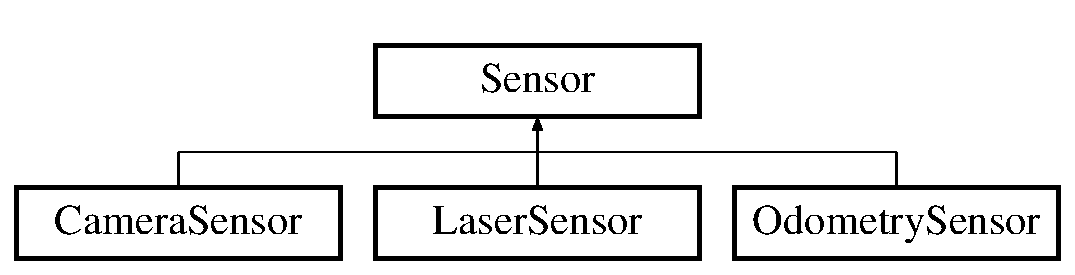
\includegraphics[height=2.000000cm]{classSensor}
\end{center}
\end{figure}
\subsection*{Public Slots}
\begin{DoxyCompactItemize}
\item 
virtual void \hyperlink{classSensor_a71fbeb7fbebe8813ad74c57e45c066bc}{onMessageReceived} (const \hyperlink{classMessage}{Message} \&message)=0
\end{DoxyCompactItemize}
\subsection*{Signals}
\begin{DoxyCompactItemize}
\item 
void \hyperlink{classSensor_a776d00dfa555b5a0b1b937c84d767bf4}{sensorData} (const \hyperlink{classMessage}{Message} \&data)
\end{DoxyCompactItemize}
\subsection*{Public Member Functions}
\begin{DoxyCompactItemize}
\item 
virtual \hyperlink{classSensor_aee8c70e7ef05ce65e7ee33686b5d7db2}{$\sim$Sensor} ()
\end{DoxyCompactItemize}
\subsection*{Protected Member Functions}
\begin{DoxyCompactItemize}
\item 
\hyperlink{classSensor_a7106654826948a6a6d76eeb37693657d}{Sensor} (QObject $\ast$parent=0)
\end{DoxyCompactItemize}


\subsection{Detailed Description}
Generic sensor interface. 

The \hyperlink{classSensor}{Sensor} virtual class defines the common interface that must be implemented by middleware classes that signal sensor data to the main application.

The particular sensorial data emitted (\hyperlink{classMessage}{Message}) is dependent on the \hyperlink{classSensor}{Sensor} implementation, hence additional information should be sought in the relative subclass documentation 

\subsection{Constructor \& Destructor Documentation}
\hypertarget{classSensor_a7106654826948a6a6d76eeb37693657d}{
\index{Sensor@{Sensor}!Sensor@{Sensor}}
\index{Sensor@{Sensor}!Sensor@{Sensor}}
\subsubsection[{Sensor}]{\setlength{\rightskip}{0pt plus 5cm}Sensor::Sensor (
\begin{DoxyParamCaption}
\item[{QObject $\ast$}]{parent = {\ttfamily 0}}
\end{DoxyParamCaption}
)\hspace{0.3cm}{\ttfamily  \mbox{[}protected\mbox{]}}}}
\label{classSensor_a7106654826948a6a6d76eeb37693657d}
Constructs a new \hyperlink{classSensor}{Sensor}


\begin{DoxyParams}{Parameters}
{\em parent} & Optional QObject parent \\
\hline
\end{DoxyParams}
\hypertarget{classSensor_aee8c70e7ef05ce65e7ee33686b5d7db2}{
\index{Sensor@{Sensor}!$\sim$Sensor@{$\sim$Sensor}}
\index{$\sim$Sensor@{$\sim$Sensor}!Sensor@{Sensor}}
\subsubsection[{$\sim$Sensor}]{\setlength{\rightskip}{0pt plus 5cm}Sensor::$\sim$Sensor (
\begin{DoxyParamCaption}
{}
\end{DoxyParamCaption}
)\hspace{0.3cm}{\ttfamily  \mbox{[}virtual\mbox{]}}}}
\label{classSensor_aee8c70e7ef05ce65e7ee33686b5d7db2}
Destroys the \hyperlink{classSensor}{Sensor} 

\subsection{Member Function Documentation}
\hypertarget{classSensor_a71fbeb7fbebe8813ad74c57e45c066bc}{
\index{Sensor@{Sensor}!onMessageReceived@{onMessageReceived}}
\index{onMessageReceived@{onMessageReceived}!Sensor@{Sensor}}
\subsubsection[{onMessageReceived}]{\setlength{\rightskip}{0pt plus 5cm}virtual void Sensor::onMessageReceived (
\begin{DoxyParamCaption}
\item[{const {\bf Message} \&}]{message}
\end{DoxyParamCaption}
)\hspace{0.3cm}{\ttfamily  \mbox{[}pure virtual, slot\mbox{]}}}}
\label{classSensor_a71fbeb7fbebe8813ad74c57e45c066bc}
This slot must be implemented by subclasses in order to receive messages from the underlying connection controller. In case the message is of interest it should be parsed and an appropriate sensorData signal should be emitted


\begin{DoxyParams}{Parameters}
{\em message} & The message received by the underlying controller \\
\hline
\end{DoxyParams}


Implemented in \hyperlink{classCameraSensor_a7ac39be83c8f461b0d6e057d8b2d4011}{CameraSensor}, \hyperlink{classLaserSensor_aa7b966f0849ce5c43920480abcae50f0}{LaserSensor}, and \hyperlink{classOdometrySensor_a31000cc77d015a52c4b9d43996ed6ae8}{OdometrySensor}.

\hypertarget{classSensor_a776d00dfa555b5a0b1b937c84d767bf4}{
\index{Sensor@{Sensor}!sensorData@{sensorData}}
\index{sensorData@{sensorData}!Sensor@{Sensor}}
\subsubsection[{sensorData}]{\setlength{\rightskip}{0pt plus 5cm}void Sensor::sensorData (
\begin{DoxyParamCaption}
\item[{const {\bf Message} \&}]{data}
\end{DoxyParamCaption}
)\hspace{0.3cm}{\ttfamily  \mbox{[}signal\mbox{]}}}}
\label{classSensor_a776d00dfa555b5a0b1b937c84d767bf4}
This signal is emitted whenever new sensor data is available. Refer to the particular \hyperlink{classSensor}{Sensor} implementation for information about the actual type of \hyperlink{classMessage}{Message} passed


\begin{DoxyParams}{Parameters}
{\em data} & The sensor data to communicate \\
\hline
\end{DoxyParams}


The documentation for this class was generated from the following files:\begin{DoxyCompactItemize}
\item 
middleware/sensor/\hyperlink{sensor_8h}{sensor.h}\item 
middleware/sensor/\hyperlink{sensor_8cpp}{sensor.cpp}\end{DoxyCompactItemize}

\hypertarget{classSensorData}{
\section{SensorData Class Reference}
\label{classSensorData}\index{SensorData@{SensorData}}
}


{\ttfamily \#include $<$sensordata.h$>$}

\subsection*{Public Member Functions}
\begin{DoxyCompactItemize}
\item 
virtual \hyperlink{classSensorData_af20d9f3e2bdd32ce2a686801694cf2a4}{$\sim$SensorData} ()
\end{DoxyCompactItemize}


\subsection{Detailed Description}
The \hyperlink{classMessage}{Message} class represents a common interface for sensorial data notification used by \hyperlink{classSensor}{Sensor} classes

\begin{DoxySeeAlso}{See also}
\hyperlink{classSensor}{Sensor} 
\end{DoxySeeAlso}


\subsection{Constructor \& Destructor Documentation}
\hypertarget{classSensorData_af20d9f3e2bdd32ce2a686801694cf2a4}{
\index{SensorData@{SensorData}!$\sim$SensorData@{$\sim$SensorData}}
\index{$\sim$SensorData@{$\sim$SensorData}!SensorData@{SensorData}}
\subsubsection[{$\sim$SensorData}]{\setlength{\rightskip}{0pt plus 5cm}virtual SensorData::$\sim$SensorData (
\begin{DoxyParamCaption}
{}
\end{DoxyParamCaption}
)\hspace{0.3cm}{\ttfamily  \mbox{[}inline, virtual\mbox{]}}}}
\label{classSensorData_af20d9f3e2bdd32ce2a686801694cf2a4}
Dummy virtual destructor needed to enable RTTI support 

The documentation for this class was generated from the following file:\begin{DoxyCompactItemize}
\item 
data/\hyperlink{sensordata_8h}{sensordata.h}\end{DoxyCompactItemize}

\hypertarget{classUPISController}{
\section{UPISController Class Reference}
\label{classUPISController}\index{UPISController@{UPISController}}
}


UPIS connection controller.  




{\ttfamily \#include $<$upiscontroller.h$>$}

Inheritance diagram for UPISController:\begin{figure}[H]
\begin{center}
\leavevmode
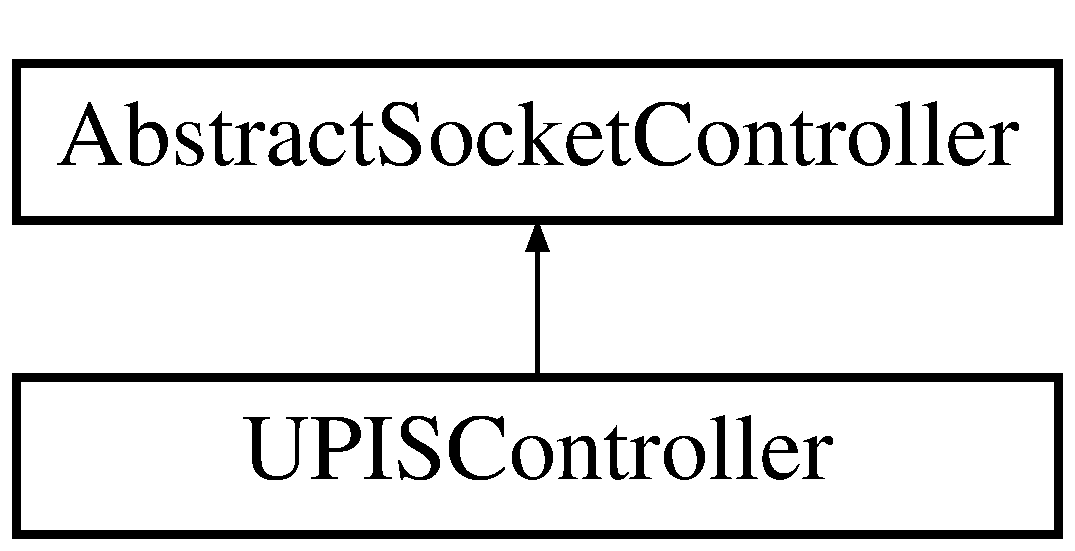
\includegraphics[height=2.000000cm]{classUPISController}
\end{center}
\end{figure}
\subsection*{Public Slots}
\begin{DoxyCompactItemize}
\item 
void \hyperlink{classUPISController_a78dcb22bf16cca05bebd9dd923c7ba28}{connectToHost} (const QString \&address, quint16 port)
\item 
void \hyperlink{classUPISController_a5d09ac4efcf74e202c905bf195f029dc}{disconnectFromHost} ()
\end{DoxyCompactItemize}
\subsection*{Signals}
\begin{DoxyCompactItemize}
\item 
void \hyperlink{classUPISController_a465e09e443e28302641ec092e285ae0a}{signalMessage} (const \hyperlink{classMessage}{Message} \&msg)
\end{DoxyCompactItemize}
\subsection*{Public Member Functions}
\begin{DoxyCompactItemize}
\item 
\hyperlink{classUPISController_a57d677d6dc0d2bbe68d93f24ec929e72}{UPISController} (double fps, int nRobot, QObject $\ast$parent=0)
\item 
virtual \hyperlink{classUPISController_a90625e6f59c386fd4b59c8652ab81977}{$\sim$UPISController} ()
\end{DoxyCompactItemize}
\subsection*{Protected Slots}
\begin{DoxyCompactItemize}
\item 
void \hyperlink{classUPISController_a20c811385172668d1071f267cc52c559}{invokeReadData} ()
\end{DoxyCompactItemize}


\subsection{Detailed Description}
UPIS connection controller. 

\hyperlink{classUPISController}{UPISController} manages the low-\/level communication to the UPIS server. A portion of the UDK draw area is periodically requested to the server and the raw image data is emitted in the form of a \hyperlink{classUPISMessage}{UPISMessage}

\begin{DoxySeeAlso}{See also}
\hyperlink{classUPISMessage}{UPISMessage} 
\end{DoxySeeAlso}


\subsection{Constructor \& Destructor Documentation}
\hypertarget{classUPISController_a57d677d6dc0d2bbe68d93f24ec929e72}{
\index{UPISController@{UPISController}!UPISController@{UPISController}}
\index{UPISController@{UPISController}!UPISController@{UPISController}}
\subsubsection[{UPISController}]{\setlength{\rightskip}{0pt plus 5cm}UPISController::UPISController (
\begin{DoxyParamCaption}
\item[{double}]{fps, }
\item[{int}]{nRobot, }
\item[{QObject $\ast$}]{parent = {\ttfamily 0}}
\end{DoxyParamCaption}
)\hspace{0.3cm}{\ttfamily  \mbox{[}explicit\mbox{]}}}}
\label{classUPISController_a57d677d6dc0d2bbe68d93f24ec929e72}
Constructs a new \hyperlink{classUPISController}{UPISController}. Two mandatory pieces of information are necessary: how frequently to request frames to UPIS (in frames per second), and the incremental number identifying the robot. The latter is necessary in order to determine what portion of the UDK draw area to request.


\begin{DoxyParams}{Parameters}
{\em fps} & The frame frequency requested \\
\hline
{\em nRobot} & Incremental number identifying the robot \\
\hline
{\em parent} & Optional QObject parent \\
\hline
\end{DoxyParams}
\hypertarget{classUPISController_a90625e6f59c386fd4b59c8652ab81977}{
\index{UPISController@{UPISController}!$\sim$UPISController@{$\sim$UPISController}}
\index{$\sim$UPISController@{$\sim$UPISController}!UPISController@{UPISController}}
\subsubsection[{$\sim$UPISController}]{\setlength{\rightskip}{0pt plus 5cm}UPISController::$\sim$UPISController (
\begin{DoxyParamCaption}
{}
\end{DoxyParamCaption}
)\hspace{0.3cm}{\ttfamily  \mbox{[}virtual\mbox{]}}}}
\label{classUPISController_a90625e6f59c386fd4b59c8652ab81977}
Destroys the \hyperlink{classUPISController}{UPISController} 

\subsection{Member Function Documentation}
\hypertarget{classUPISController_a78dcb22bf16cca05bebd9dd923c7ba28}{
\index{UPISController@{UPISController}!connectToHost@{connectToHost}}
\index{connectToHost@{connectToHost}!UPISController@{UPISController}}
\subsubsection[{connectToHost}]{\setlength{\rightskip}{0pt plus 5cm}void UPISController::connectToHost (
\begin{DoxyParamCaption}
\item[{const QString \&}]{address, }
\item[{quint16}]{port}
\end{DoxyParamCaption}
)\hspace{0.3cm}{\ttfamily  \mbox{[}virtual, slot\mbox{]}}}}
\label{classUPISController_a78dcb22bf16cca05bebd9dd923c7ba28}
Establishes a connection to the specified host/port. This method is non-\/blocking, hence, before any communication is attempted the application should wait for the \hyperlink{classAbstractSocketController_af09d800cea400d85c29e07322faaf934}{signalConnected()} signal


\begin{DoxyParams}{Parameters}
{\em address} & IP address or hostname of the target host \\
\hline
{\em port} & TCP port to connect to \\
\hline
\end{DoxyParams}


Overridden in order to start frame request timer 

Reimplemented from \hyperlink{classAbstractSocketController_a13af2e22144c96860f6a3975365dc1ff}{AbstractSocketController}.

\hypertarget{classUPISController_a5d09ac4efcf74e202c905bf195f029dc}{
\index{UPISController@{UPISController}!disconnectFromHost@{disconnectFromHost}}
\index{disconnectFromHost@{disconnectFromHost}!UPISController@{UPISController}}
\subsubsection[{disconnectFromHost}]{\setlength{\rightskip}{0pt plus 5cm}void UPISController::disconnectFromHost (
\begin{DoxyParamCaption}
{}
\end{DoxyParamCaption}
)\hspace{0.3cm}{\ttfamily  \mbox{[}virtual, slot\mbox{]}}}}
\label{classUPISController_a5d09ac4efcf74e202c905bf195f029dc}
Terminates the connection to the host. The actual disconnection notification is emitted through the \hyperlink{classAbstractSocketController_a5d1dee9948125660e67a671cabed122f}{signalDisconnected()} signal 

Overridden in order to stop frame request timer 

Reimplemented from \hyperlink{classAbstractSocketController_a399c565654a03e6cb352dfc576460ff7}{AbstractSocketController}.

\hypertarget{classUPISController_a20c811385172668d1071f267cc52c559}{
\index{UPISController@{UPISController}!invokeReadData@{invokeReadData}}
\index{invokeReadData@{invokeReadData}!UPISController@{UPISController}}
\subsubsection[{invokeReadData}]{\setlength{\rightskip}{0pt plus 5cm}void UPISController::invokeReadData (
\begin{DoxyParamCaption}
{}
\end{DoxyParamCaption}
)\hspace{0.3cm}{\ttfamily  \mbox{[}protected, virtual, slot\mbox{]}}}}
\label{classUPISController_a20c811385172668d1071f267cc52c559}
\hyperlink{classAbstractSocketController_a3816ceb3b12f0028dea99d010349ec41}{AbstractSocketController::invokeReadData()} implementation for \hyperlink{classUPISController}{UPISController} 

Implements \hyperlink{classAbstractSocketController_a3816ceb3b12f0028dea99d010349ec41}{AbstractSocketController}.

\hypertarget{classUPISController_a465e09e443e28302641ec092e285ae0a}{
\index{UPISController@{UPISController}!signalMessage@{signalMessage}}
\index{signalMessage@{signalMessage}!UPISController@{UPISController}}
\subsubsection[{signalMessage}]{\setlength{\rightskip}{0pt plus 5cm}void UPISController::signalMessage (
\begin{DoxyParamCaption}
\item[{const {\bf Message} \&}]{msg}
\end{DoxyParamCaption}
)\hspace{0.3cm}{\ttfamily  \mbox{[}signal\mbox{]}}}}
\label{classUPISController_a465e09e443e28302641ec092e285ae0a}
Signals a \hyperlink{classMessage}{Message} to the connected Sensor(s). The actual object provided is an instance of \hyperlink{classUPISMessage}{UPISMessage} containing raw image data; the definition of the signal reports a generic \hyperlink{classMessage}{Message} in order to be compatible with the slot definition of the \hyperlink{classSensor}{Sensor} interface


\begin{DoxyParams}{Parameters}
{\em msg} & \hyperlink{classMessage}{Message} containing raw image data \\
\hline
\end{DoxyParams}


The documentation for this class was generated from the following files:\begin{DoxyCompactItemize}
\item 
connection/\hyperlink{upiscontroller_8h}{upiscontroller.h}\item 
connection/\hyperlink{upiscontroller_8cpp}{upiscontroller.cpp}\end{DoxyCompactItemize}

\hypertarget{classUPISMessage}{
\section{UPISMessage Class Reference}
\label{classUPISMessage}\index{UPISMessage@{UPISMessage}}
}


\hyperlink{classMessage}{Message} representing data sent from UPIS.  




{\ttfamily \#include $<$upismessage.h$>$}

Inheritance diagram for UPISMessage:\begin{figure}[H]
\begin{center}
\leavevmode
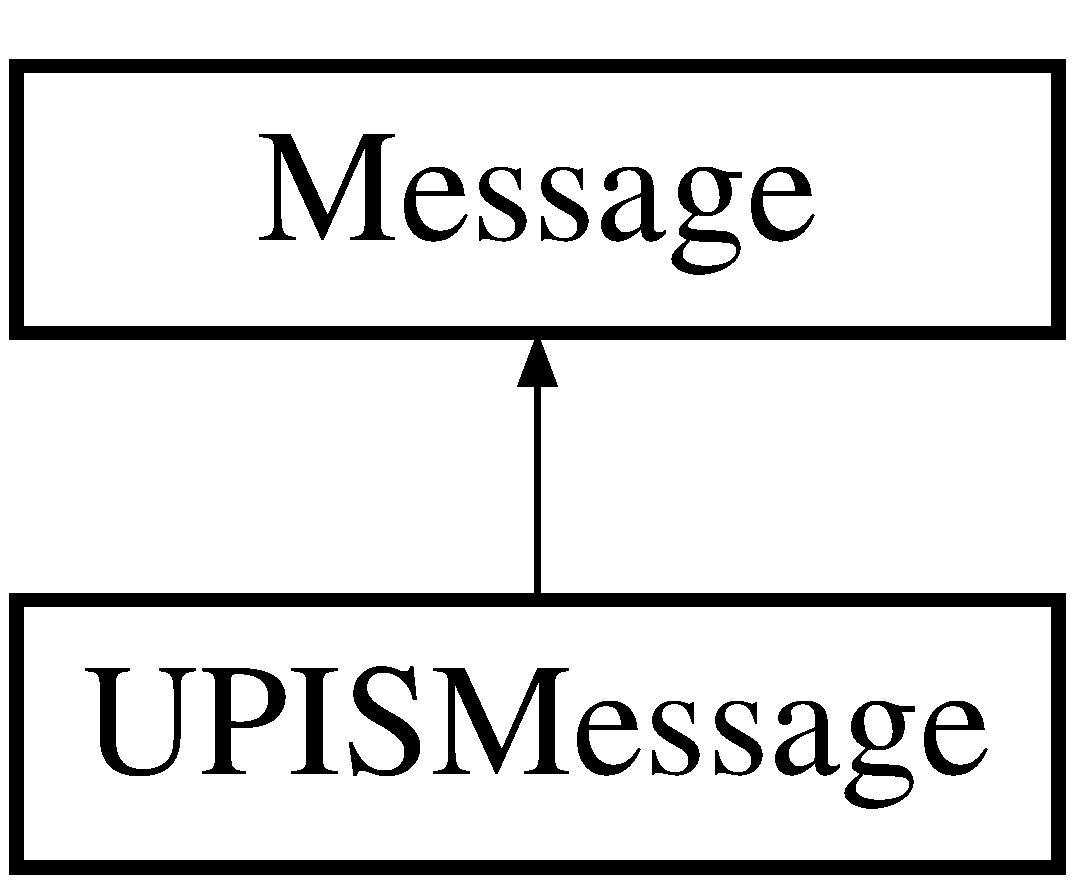
\includegraphics[height=2.000000cm]{classUPISMessage}
\end{center}
\end{figure}
\subsection*{Public Member Functions}
\begin{DoxyCompactItemize}
\item 
\hyperlink{classUPISMessage_aa3cb85cd725551f1bc74f09413f8e9f2}{UPISMessage} (bool jpeg, const QByteArray \&binData)
\item 
bool \hyperlink{classUPISMessage_a48073be902fb18f8240a1eae81636cb8}{isJPEG} () const 
\item 
bool \hyperlink{classUPISMessage_a71b6912bd6db1175d9102a730af2e724}{isRAW} () const 
\end{DoxyCompactItemize}


\subsection{Detailed Description}
\hyperlink{classMessage}{Message} representing data sent from UPIS. 

The \hyperlink{classUPISMessage}{UPISMessage} class represents a message returned by UPIS. It is simply a raw image byte array with the additional property of being able to distinguish between JPEG and RAW image data.

\begin{DoxySeeAlso}{See also}
\hyperlink{classUPISController}{UPISController} 
\end{DoxySeeAlso}


\subsection{Constructor \& Destructor Documentation}
\hypertarget{classUPISMessage_aa3cb85cd725551f1bc74f09413f8e9f2}{
\index{UPISMessage@{UPISMessage}!UPISMessage@{UPISMessage}}
\index{UPISMessage@{UPISMessage}!UPISMessage@{UPISMessage}}
\subsubsection[{UPISMessage}]{\setlength{\rightskip}{0pt plus 5cm}UPISMessage::UPISMessage (
\begin{DoxyParamCaption}
\item[{bool}]{jpeg, }
\item[{const QByteArray \&}]{binData}
\end{DoxyParamCaption}
)}}
\label{classUPISMessage_aa3cb85cd725551f1bc74f09413f8e9f2}
Initialises a new \hyperlink{classUPISMessage}{UPISMessage} with data content binData


\begin{DoxyParams}{Parameters}
{\em jpeg} & true if the content is JPEG data, false if RAW data \\
\hline
{\em binData} & Binary image data \\
\hline
\end{DoxyParams}


\subsection{Member Function Documentation}
\hypertarget{classUPISMessage_a48073be902fb18f8240a1eae81636cb8}{
\index{UPISMessage@{UPISMessage}!isJPEG@{isJPEG}}
\index{isJPEG@{isJPEG}!UPISMessage@{UPISMessage}}
\subsubsection[{isJPEG}]{\setlength{\rightskip}{0pt plus 5cm}bool UPISMessage::isJPEG (
\begin{DoxyParamCaption}
{}
\end{DoxyParamCaption}
) const}}
\label{classUPISMessage_a48073be902fb18f8240a1eae81636cb8}
\begin{DoxyReturn}{Returns}
true if the binary data is in JPEG format, false otherwise 
\end{DoxyReturn}
\hypertarget{classUPISMessage_a71b6912bd6db1175d9102a730af2e724}{
\index{UPISMessage@{UPISMessage}!isRAW@{isRAW}}
\index{isRAW@{isRAW}!UPISMessage@{UPISMessage}}
\subsubsection[{isRAW}]{\setlength{\rightskip}{0pt plus 5cm}bool UPISMessage::isRAW (
\begin{DoxyParamCaption}
{}
\end{DoxyParamCaption}
) const}}
\label{classUPISMessage_a71b6912bd6db1175d9102a730af2e724}
Logical negation of \hyperlink{classUPISMessage_a48073be902fb18f8240a1eae81636cb8}{isJPEG()}

\begin{DoxyReturn}{Returns}
true is the binary data is in RAW format, false otherwise 
\end{DoxyReturn}


The documentation for this class was generated from the following files:\begin{DoxyCompactItemize}
\item 
data/\hyperlink{upismessage_8h}{upismessage.h}\item 
data/\hyperlink{upismessage_8cpp}{upismessage.cpp}\end{DoxyCompactItemize}

\hypertarget{classUSARController}{
\section{USARController Class Reference}
\label{classUSARController}\index{USARController@{USARController}}
}


USARSim connection controller.  




{\ttfamily \#include $<$usarcontroller.h$>$}

Inheritance diagram for USARController:\begin{figure}[H]
\begin{center}
\leavevmode
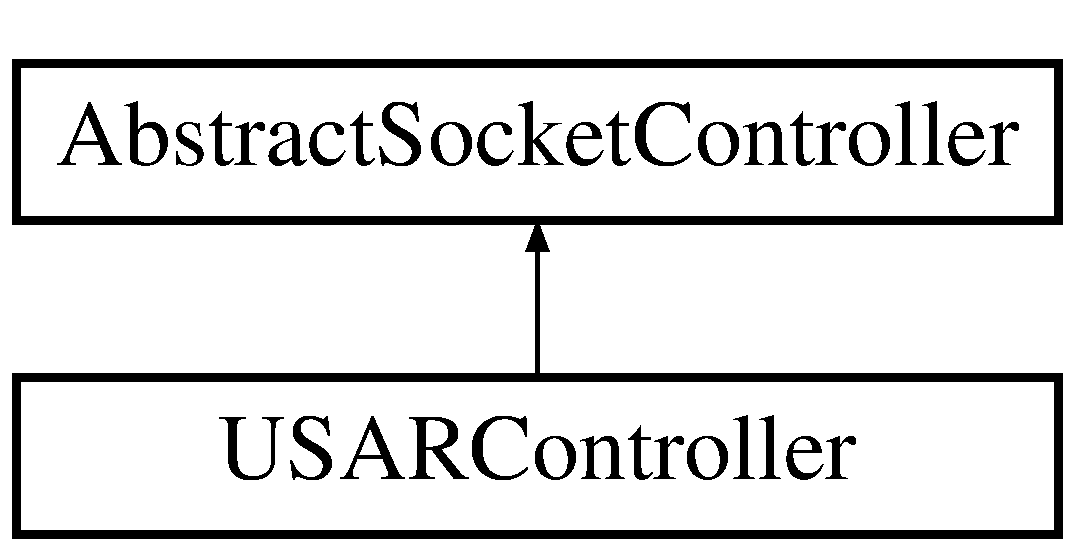
\includegraphics[height=2.000000cm]{classUSARController}
\end{center}
\end{figure}
\subsection*{Public Slots}
\begin{DoxyCompactItemize}
\item 
void \hyperlink{classUSARController_a2becbd888b35304051cc2095570b3b18}{sendMessage} (const \hyperlink{classMessage}{Message} \&msg)
\end{DoxyCompactItemize}
\subsection*{Signals}
\begin{DoxyCompactItemize}
\item 
void \hyperlink{classUSARController_a42e81ce338bb7799c42ca968369aaf7b}{signalMessage} (const \hyperlink{classMessage}{Message} \&msg)
\end{DoxyCompactItemize}
\subsection*{Public Member Functions}
\begin{DoxyCompactItemize}
\item 
\hyperlink{classUSARController_ac5c82f3819f4a34b00cfcc63547ab2a6}{USARController} (QObject $\ast$parent=0)
\item 
virtual \hyperlink{classUSARController_a450f87dd480cc0c0895255fa4bebf869}{$\sim$USARController} ()
\end{DoxyCompactItemize}
\subsection*{Protected Slots}
\begin{DoxyCompactItemize}
\item 
void \hyperlink{classUSARController_aea2a9dde924c625b83da33a6848f41f0}{invokeReadData} ()
\end{DoxyCompactItemize}


\subsection{Detailed Description}
USARSim connection controller. 

\hyperlink{classUSARController}{USARController} manages the low-\/level communication to the USARSim server. A signal is emitted every time a message is received from the server, conversely the controller will forward a message to the server in case a connected \hyperlink{classDriver}{Driver} has requested so. Both input and output communication data is encapsulated in \hyperlink{classUSARMessage}{USARMessage} instances

\begin{DoxySeeAlso}{See also}
\hyperlink{classUSARMessage}{USARMessage} 
\end{DoxySeeAlso}


\subsection{Constructor \& Destructor Documentation}
\hypertarget{classUSARController_ac5c82f3819f4a34b00cfcc63547ab2a6}{
\index{USARController@{USARController}!USARController@{USARController}}
\index{USARController@{USARController}!USARController@{USARController}}
\subsubsection[{USARController}]{\setlength{\rightskip}{0pt plus 5cm}USARController::USARController (
\begin{DoxyParamCaption}
\item[{QObject $\ast$}]{parent = {\ttfamily 0}}
\end{DoxyParamCaption}
)\hspace{0.3cm}{\ttfamily  \mbox{[}explicit\mbox{]}}}}
\label{classUSARController_ac5c82f3819f4a34b00cfcc63547ab2a6}
Constructs a new \hyperlink{classUSARController}{USARController}


\begin{DoxyParams}{Parameters}
{\em parent} & Optional QObject parent \\
\hline
\end{DoxyParams}
\hypertarget{classUSARController_a450f87dd480cc0c0895255fa4bebf869}{
\index{USARController@{USARController}!$\sim$USARController@{$\sim$USARController}}
\index{$\sim$USARController@{$\sim$USARController}!USARController@{USARController}}
\subsubsection[{$\sim$USARController}]{\setlength{\rightskip}{0pt plus 5cm}USARController::$\sim$USARController (
\begin{DoxyParamCaption}
{}
\end{DoxyParamCaption}
)\hspace{0.3cm}{\ttfamily  \mbox{[}virtual\mbox{]}}}}
\label{classUSARController_a450f87dd480cc0c0895255fa4bebf869}
Destroys the \hyperlink{classUSARController}{USARController} 

\subsection{Member Function Documentation}
\hypertarget{classUSARController_aea2a9dde924c625b83da33a6848f41f0}{
\index{USARController@{USARController}!invokeReadData@{invokeReadData}}
\index{invokeReadData@{invokeReadData}!USARController@{USARController}}
\subsubsection[{invokeReadData}]{\setlength{\rightskip}{0pt plus 5cm}void USARController::invokeReadData (
\begin{DoxyParamCaption}
{}
\end{DoxyParamCaption}
)\hspace{0.3cm}{\ttfamily  \mbox{[}protected, virtual, slot\mbox{]}}}}
\label{classUSARController_aea2a9dde924c625b83da33a6848f41f0}
\hyperlink{classAbstractSocketController_a3816ceb3b12f0028dea99d010349ec41}{AbstractSocketController::invokeReadData()} implementation for \hyperlink{classUSARController}{USARController} 

Implements \hyperlink{classAbstractSocketController_a3816ceb3b12f0028dea99d010349ec41}{AbstractSocketController}.

\hypertarget{classUSARController_a2becbd888b35304051cc2095570b3b18}{
\index{USARController@{USARController}!sendMessage@{sendMessage}}
\index{sendMessage@{sendMessage}!USARController@{USARController}}
\subsubsection[{sendMessage}]{\setlength{\rightskip}{0pt plus 5cm}void USARController::sendMessage (
\begin{DoxyParamCaption}
\item[{const {\bf Message} \&}]{msg}
\end{DoxyParamCaption}
)\hspace{0.3cm}{\ttfamily  \mbox{[}slot\mbox{]}}}}
\label{classUSARController_a2becbd888b35304051cc2095570b3b18}
Slot aimed at sending a message to the USARSim message. This method expects a \hyperlink{classUSARMessage}{USARMessage} as input argument, any different object will be quietly ignored. The definition of the slot reports a generic \hyperlink{classMessage}{Message} in order to be compatible with the corresponding signal definition of the \hyperlink{classDriver}{Driver} interface


\begin{DoxyParams}{Parameters}
{\em msg} & \hyperlink{classMessage}{Message} containing information to send to USARSim \\
\hline
\end{DoxyParams}
\hypertarget{classUSARController_a42e81ce338bb7799c42ca968369aaf7b}{
\index{USARController@{USARController}!signalMessage@{signalMessage}}
\index{signalMessage@{signalMessage}!USARController@{USARController}}
\subsubsection[{signalMessage}]{\setlength{\rightskip}{0pt plus 5cm}void USARController::signalMessage (
\begin{DoxyParamCaption}
\item[{const {\bf Message} \&}]{msg}
\end{DoxyParamCaption}
)\hspace{0.3cm}{\ttfamily  \mbox{[}signal\mbox{]}}}}
\label{classUSARController_a42e81ce338bb7799c42ca968369aaf7b}
Signals a \hyperlink{classMessage}{Message} to the connected Sensor(s). The actual object provided is an instance of \hyperlink{classUSARMessage}{USARMessage} containing the information sent by the server; the definition of the signal reports a generic \hyperlink{classMessage}{Message} in order to be compatible with thecorresponding slot definition of the \hyperlink{classSensor}{Sensor} interface


\begin{DoxyParams}{Parameters}
{\em msg} & \hyperlink{classMessage}{Message} containing information sent by USARSim \\
\hline
\end{DoxyParams}


The documentation for this class was generated from the following files:\begin{DoxyCompactItemize}
\item 
connection/\hyperlink{usarcontroller_8h}{usarcontroller.h}\item 
connection/\hyperlink{usarcontroller_8cpp}{usarcontroller.cpp}\end{DoxyCompactItemize}

\hypertarget{classUSARMessage}{
\section{USARMessage Class Reference}
\label{classUSARMessage}\index{USARMessage@{USARMessage}}
}


\hyperlink{classMessage}{Message} representing data sent to and from USARSim.  




{\ttfamily \#include $<$usarmessage.h$>$}

Inheritance diagram for USARMessage:\begin{figure}[H]
\begin{center}
\leavevmode
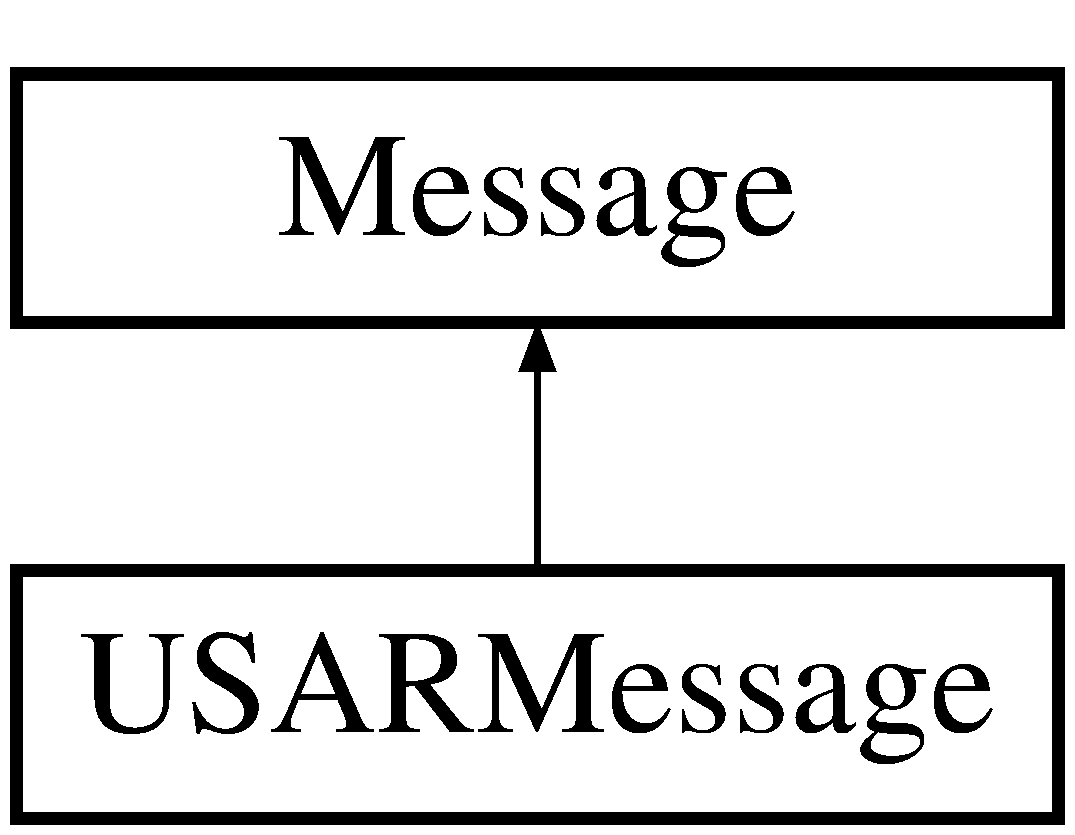
\includegraphics[height=2.000000cm]{classUSARMessage}
\end{center}
\end{figure}
\subsection*{Public Member Functions}
\begin{DoxyCompactItemize}
\item 
\hyperlink{classUSARMessage_a9e9a5ff3fa214118795f8ff497d405cd}{USARMessage} ()
\item 
\hyperlink{classUSARMessage_a15feacf7b822e859023b7951104d2c86}{USARMessage} (const QString \&line)
\item 
\hyperlink{classUSARMessage_a773cca2f8b7144ee91607f9a06de8b87}{USARMessage} (const \hyperlink{classUSARMessage}{USARMessage} \&message)
\item 
virtual \hyperlink{classUSARMessage_ae1b97a8729759a96269a7a6094dc16d1}{$\sim$USARMessage} ()
\item 
\hyperlink{classUSARMessage_a37cb1728fb9fba59a8d46376ef4ff06f}{operator QString} () const 
\item 
void \hyperlink{classUSARMessage_a758f2f40962494e9d7849b3f9a480599}{setType} (const QString \&type)
\item 
const QString \& \hyperlink{classUSARMessage_ab71d4e8b5cd81b7b6567936fb4614aaf}{getType} () const 
\item 
const QString \& \hyperlink{classUSARMessage_a75f24312fd0d5ae95c2439d31e11d9f1}{operator\mbox{[}$\,$\mbox{]}} (const QString \&key) const 
\item 
QString \& \hyperlink{classUSARMessage_af7df32828ebbac479f34d769575e4ea1}{operator\mbox{[}$\,$\mbox{]}} (const QString \&key)
\item 
void \hyperlink{classUSARMessage_af98c3d21afaba3456bd8eab56d92de1a}{insert} (const QString \&key, const QString \&value)
\item 
bool \hyperlink{classUSARMessage_aa86ec4c02f60f20d65db97c062c601b2}{contains} (const QString \&key) const 
\item 
const QList$<$ QString $>$ \& \hyperlink{classUSARMessage_a449ec98406459bad6ed7fc0e58e105f8}{keys} () const 
\end{DoxyCompactItemize}


\subsection{Detailed Description}
\hyperlink{classMessage}{Message} representing data sent to and from USARSim. 

The \hyperlink{classUSARMessage}{USARMessage} class represents a message aimed towards, or signalled by \hyperlink{classUSARController}{USARController}. The class is effectively a hash table containing key-\/value pairs and an additional string representing the type of the message (e.g. INFO, SEN, STA, DRIVE, ...). When parsing a message the order of the parameters is preserved; similarly when constructing a new message with the provided methods the ordering of the parameters is determined by the order in which the key/value pairs were inserted

\begin{DoxySeeAlso}{See also}
\hyperlink{classUSARController}{USARController} 
\end{DoxySeeAlso}


\subsection{Constructor \& Destructor Documentation}
\hypertarget{classUSARMessage_a9e9a5ff3fa214118795f8ff497d405cd}{
\index{USARMessage@{USARMessage}!USARMessage@{USARMessage}}
\index{USARMessage@{USARMessage}!USARMessage@{USARMessage}}
\subsubsection[{USARMessage}]{\setlength{\rightskip}{0pt plus 5cm}USARMessage::USARMessage (
\begin{DoxyParamCaption}
{}
\end{DoxyParamCaption}
)}}
\label{classUSARMessage_a9e9a5ff3fa214118795f8ff497d405cd}
Initialises an empty \hyperlink{classUSARMessage}{USARMessage} \hypertarget{classUSARMessage_a15feacf7b822e859023b7951104d2c86}{
\index{USARMessage@{USARMessage}!USARMessage@{USARMessage}}
\index{USARMessage@{USARMessage}!USARMessage@{USARMessage}}
\subsubsection[{USARMessage}]{\setlength{\rightskip}{0pt plus 5cm}USARMessage::USARMessage (
\begin{DoxyParamCaption}
\item[{const QString \&}]{line}
\end{DoxyParamCaption}
)\hspace{0.3cm}{\ttfamily  \mbox{[}explicit\mbox{]}}}}
\label{classUSARMessage_a15feacf7b822e859023b7951104d2c86}
Initialises an \hyperlink{classUSARMessage}{USARMessage} from a string serialised representation of a USARSim message, the input is parsed and the type and key-\/value pairs are filled


\begin{DoxyParams}{Parameters}
{\em line} & The input string serialised USARSim message \\
\hline
\end{DoxyParams}
\hypertarget{classUSARMessage_a773cca2f8b7144ee91607f9a06de8b87}{
\index{USARMessage@{USARMessage}!USARMessage@{USARMessage}}
\index{USARMessage@{USARMessage}!USARMessage@{USARMessage}}
\subsubsection[{USARMessage}]{\setlength{\rightskip}{0pt plus 5cm}USARMessage::USARMessage (
\begin{DoxyParamCaption}
\item[{const {\bf USARMessage} \&}]{message}
\end{DoxyParamCaption}
)}}
\label{classUSARMessage_a773cca2f8b7144ee91607f9a06de8b87}
Initialises an \hyperlink{classUSARMessage}{USARMessage} from another existing one


\begin{DoxyParams}{Parameters}
{\em message} & The \hyperlink{classUSARMessage}{USARMessage} to clone \\
\hline
\end{DoxyParams}
\hypertarget{classUSARMessage_ae1b97a8729759a96269a7a6094dc16d1}{
\index{USARMessage@{USARMessage}!$\sim$USARMessage@{$\sim$USARMessage}}
\index{$\sim$USARMessage@{$\sim$USARMessage}!USARMessage@{USARMessage}}
\subsubsection[{$\sim$USARMessage}]{\setlength{\rightskip}{0pt plus 5cm}USARMessage::$\sim$USARMessage (
\begin{DoxyParamCaption}
{}
\end{DoxyParamCaption}
)\hspace{0.3cm}{\ttfamily  \mbox{[}virtual\mbox{]}}}}
\label{classUSARMessage_ae1b97a8729759a96269a7a6094dc16d1}
Destroys the \hyperlink{classUSARMessage}{USARMessage} 

\subsection{Member Function Documentation}
\hypertarget{classUSARMessage_aa86ec4c02f60f20d65db97c062c601b2}{
\index{USARMessage@{USARMessage}!contains@{contains}}
\index{contains@{contains}!USARMessage@{USARMessage}}
\subsubsection[{contains}]{\setlength{\rightskip}{0pt plus 5cm}bool USARMessage::contains (
\begin{DoxyParamCaption}
\item[{const QString \&}]{key}
\end{DoxyParamCaption}
) const}}
\label{classUSARMessage_aa86ec4c02f60f20d65db97c062c601b2}
Checks whether a parameter key exists in the message or not


\begin{DoxyParams}{Parameters}
{\em key} & Input parameter key \\
\hline
\end{DoxyParams}
\begin{DoxyReturn}{Returns}
true if key exists in the message, false otherwise 
\end{DoxyReturn}
\hypertarget{classUSARMessage_ab71d4e8b5cd81b7b6567936fb4614aaf}{
\index{USARMessage@{USARMessage}!getType@{getType}}
\index{getType@{getType}!USARMessage@{USARMessage}}
\subsubsection[{getType}]{\setlength{\rightskip}{0pt plus 5cm}const QString \& USARMessage::getType (
\begin{DoxyParamCaption}
{}
\end{DoxyParamCaption}
) const}}
\label{classUSARMessage_ab71d4e8b5cd81b7b6567936fb4614aaf}
Retrieves the message type

\begin{DoxyReturn}{Returns}
\hyperlink{classMessage}{Message} type 
\end{DoxyReturn}
\hypertarget{classUSARMessage_af98c3d21afaba3456bd8eab56d92de1a}{
\index{USARMessage@{USARMessage}!insert@{insert}}
\index{insert@{insert}!USARMessage@{USARMessage}}
\subsubsection[{insert}]{\setlength{\rightskip}{0pt plus 5cm}void USARMessage::insert (
\begin{DoxyParamCaption}
\item[{const QString \&}]{key, }
\item[{const QString \&}]{value}
\end{DoxyParamCaption}
)}}
\label{classUSARMessage_af98c3d21afaba3456bd8eab56d92de1a}
Adds a new key/value pair to the message after the existing ones (ordered)


\begin{DoxyParams}{Parameters}
{\em key} & Input parameter key \\
\hline
{\em value} & Value associated to the key \\
\hline
\end{DoxyParams}
\hypertarget{classUSARMessage_a449ec98406459bad6ed7fc0e58e105f8}{
\index{USARMessage@{USARMessage}!keys@{keys}}
\index{keys@{keys}!USARMessage@{USARMessage}}
\subsubsection[{keys}]{\setlength{\rightskip}{0pt plus 5cm}const QList$<$ QString $>$ \& USARMessage::keys (
\begin{DoxyParamCaption}
{}
\end{DoxyParamCaption}
) const}}
\label{classUSARMessage_a449ec98406459bad6ed7fc0e58e105f8}
Provides const reference to the list of parameter keys in the message, sorted in order of insertion (or parsing)

\begin{DoxyReturn}{Returns}
Ordered parameter keys 
\end{DoxyReturn}
\hypertarget{classUSARMessage_a37cb1728fb9fba59a8d46376ef4ff06f}{
\index{USARMessage@{USARMessage}!operator QString@{operator QString}}
\index{operator QString@{operator QString}!USARMessage@{USARMessage}}
\subsubsection[{operator QString}]{\setlength{\rightskip}{0pt plus 5cm}USARMessage::operator QString (
\begin{DoxyParamCaption}
{}
\end{DoxyParamCaption}
) const}}
\label{classUSARMessage_a37cb1728fb9fba59a8d46376ef4ff06f}
Serialises the \hyperlink{classUSARMessage}{USARMessage} into a valid string which adheres to the USARSim standard

\begin{DoxyReturn}{Returns}
The serialised string 
\end{DoxyReturn}
\hypertarget{classUSARMessage_a75f24312fd0d5ae95c2439d31e11d9f1}{
\index{USARMessage@{USARMessage}!operator\mbox{[}\mbox{]}@{operator[]}}
\index{operator\mbox{[}\mbox{]}@{operator[]}!USARMessage@{USARMessage}}
\subsubsection[{operator[]}]{\setlength{\rightskip}{0pt plus 5cm}const QString \& USARMessage::operator\mbox{[}$\,$\mbox{]} (
\begin{DoxyParamCaption}
\item[{const QString \&}]{key}
\end{DoxyParamCaption}
) const}}
\label{classUSARMessage_a75f24312fd0d5ae95c2439d31e11d9f1}
Returns a constant reference to the value of the parameter specified by key


\begin{DoxyParams}{Parameters}
{\em key} & Input parameter key \\
\hline
\end{DoxyParams}
\begin{DoxyReturn}{Returns}
Constant reference to value indexed by key 
\end{DoxyReturn}
\hypertarget{classUSARMessage_af7df32828ebbac479f34d769575e4ea1}{
\index{USARMessage@{USARMessage}!operator\mbox{[}\mbox{]}@{operator[]}}
\index{operator\mbox{[}\mbox{]}@{operator[]}!USARMessage@{USARMessage}}
\subsubsection[{operator[]}]{\setlength{\rightskip}{0pt plus 5cm}QString \& USARMessage::operator\mbox{[}$\,$\mbox{]} (
\begin{DoxyParamCaption}
\item[{const QString \&}]{key}
\end{DoxyParamCaption}
)}}
\label{classUSARMessage_af7df32828ebbac479f34d769575e4ea1}
Returns a modifiable reference to the value of the parameter specified by key. If the key does not exist a new entry is created


\begin{DoxyParams}{Parameters}
{\em key} & Input parameter key \\
\hline
\end{DoxyParams}
\begin{DoxyReturn}{Returns}
Modifiable reference to value indexed by key 
\end{DoxyReturn}
\hypertarget{classUSARMessage_a758f2f40962494e9d7849b3f9a480599}{
\index{USARMessage@{USARMessage}!setType@{setType}}
\index{setType@{setType}!USARMessage@{USARMessage}}
\subsubsection[{setType}]{\setlength{\rightskip}{0pt plus 5cm}void USARMessage::setType (
\begin{DoxyParamCaption}
\item[{const QString \&}]{type}
\end{DoxyParamCaption}
)}}
\label{classUSARMessage_a758f2f40962494e9d7849b3f9a480599}
Sets the message type


\begin{DoxyParams}{Parameters}
{\em type} & \hyperlink{classMessage}{Message} type \\
\hline
\end{DoxyParams}


The documentation for this class was generated from the following files:\begin{DoxyCompactItemize}
\item 
data/\hyperlink{usarmessage_8h}{usarmessage.h}\item 
data/\hyperlink{usarmessage_8cpp}{usarmessage.cpp}\end{DoxyCompactItemize}

\chapter{File Documentation}
\hypertarget{abstractsocketcontroller_8cpp}{
\section{connection/abstractsocketcontroller.cpp File Reference}
\label{abstractsocketcontroller_8cpp}\index{connection/abstractsocketcontroller.cpp@{connection/abstractsocketcontroller.cpp}}
}
{\ttfamily \#include \char`\"{}abstractsocketcontroller.h\char`\"{}}\par
{\ttfamily \#include \char`\"{}data/usarmessage.h\char`\"{}}\par
{\ttfamily \#include $<$QHostAddress$>$}\par

\hypertarget{abstractsocketcontroller_8h}{
\section{connection/abstractsocketcontroller.h File Reference}
\label{abstractsocketcontroller_8h}\index{connection/abstractsocketcontroller.h@{connection/abstractsocketcontroller.h}}
}
{\ttfamily \#include $<$QString$>$}\par
{\ttfamily \#include $<$QTcpSocket$>$}\par
\subsection*{Classes}
\begin{DoxyCompactItemize}
\item 
class \hyperlink{classAbstractSocketController}{AbstractSocketController}
\begin{DoxyCompactList}\small\item\em Shared functionalities for socket based controllers. \end{DoxyCompactList}\end{DoxyCompactItemize}

\hypertarget{upiscontroller_8cpp}{
\section{connection/upiscontroller.cpp File Reference}
\label{upiscontroller_8cpp}\index{connection/upiscontroller.cpp@{connection/upiscontroller.cpp}}
}
{\ttfamily \#include \char`\"{}upiscontroller.h\char`\"{}}\par
{\ttfamily \#include $<$QHostAddress$>$}\par
{\ttfamily \#include \char`\"{}data/usarmessage.h\char`\"{}}\par
{\ttfamily \#include \char`\"{}shared/utilities.h\char`\"{}}\par
{\ttfamily \#include \char`\"{}data/upismessage.h\char`\"{}}\par

\hypertarget{upiscontroller_8h}{
\section{connection/upiscontroller.h File Reference}
\label{upiscontroller_8h}\index{connection/upiscontroller.h@{connection/upiscontroller.h}}
}
{\ttfamily \#include \char`\"{}abstractsocketcontroller.h\char`\"{}}\par
{\ttfamily \#include \char`\"{}data/message.h\char`\"{}}\par
{\ttfamily \#include \char`\"{}shared/constants.h\char`\"{}}\par
{\ttfamily \#include $<$QByteArray$>$}\par
{\ttfamily \#include $<$QTimer$>$}\par
\subsection*{Classes}
\begin{DoxyCompactItemize}
\item 
class \hyperlink{classUPISController}{UPISController}
\begin{DoxyCompactList}\small\item\em UPIS connection controller. \end{DoxyCompactList}\end{DoxyCompactItemize}

\hypertarget{usarcontroller_8cpp}{
\section{connection/usarcontroller.cpp File Reference}
\label{usarcontroller_8cpp}\index{connection/usarcontroller.cpp@{connection/usarcontroller.cpp}}
}
{\ttfamily \#include \char`\"{}usarcontroller.h\char`\"{}}\par
{\ttfamily \#include \char`\"{}data/usarmessage.h\char`\"{}}\par
{\ttfamily \#include $<$typeinfo$>$}\par

\hypertarget{usarcontroller_8h}{
\section{connection/usarcontroller.h File Reference}
\label{usarcontroller_8h}\index{connection/usarcontroller.h@{connection/usarcontroller.h}}
}
{\ttfamily \#include \char`\"{}abstractsocketcontroller.h\char`\"{}}\par
{\ttfamily \#include \char`\"{}data/message.h\char`\"{}}\par
\subsection*{Classes}
\begin{DoxyCompactItemize}
\item 
class \hyperlink{classUSARController}{USARController}
\begin{DoxyCompactList}\small\item\em USARSim connection controller. \end{DoxyCompactList}\end{DoxyCompactItemize}

\hypertarget{action_8cpp}{
\section{data/action.cpp File Reference}
\label{action_8cpp}\index{data/action.cpp@{data/action.cpp}}
}
{\ttfamily \#include \char`\"{}action.h\char`\"{}}\par

\hypertarget{action_8h}{
\section{data/action.h File Reference}
\label{action_8h}\index{data/action.h@{data/action.h}}
}
{\ttfamily \#include $<$QObject$>$}\par
\subsection*{Classes}
\begin{DoxyCompactItemize}
\item 
class \hyperlink{classAction}{Action}
\end{DoxyCompactItemize}

\hypertarget{cameradata_8cpp}{
\section{data/cameradata.cpp File Reference}
\label{cameradata_8cpp}\index{data/cameradata.cpp@{data/cameradata.cpp}}
}
{\ttfamily \#include \char`\"{}cameradata.h\char`\"{}}\par

\hypertarget{cameradata_8h}{
\section{data/cameradata.h File Reference}
\label{cameradata_8h}\index{data/cameradata.h@{data/cameradata.h}}
}
{\ttfamily \#include \char`\"{}message.h\char`\"{}}\par
{\ttfamily \#include $<$QImage$>$}\par
\subsection*{Classes}
\begin{DoxyCompactItemize}
\item 
class \hyperlink{classCameraData}{CameraData}
\begin{DoxyCompactList}\small\item\em Camera data message. \end{DoxyCompactList}\end{DoxyCompactItemize}

\hypertarget{laserdata_8cpp}{
\section{data/laserdata.cpp File Reference}
\label{laserdata_8cpp}\index{data/laserdata.cpp@{data/laserdata.cpp}}
}
{\ttfamily \#include \char`\"{}laserdata.h\char`\"{}}\par

\hypertarget{laserdata_8h}{
\section{data/laserdata.h File Reference}
\label{laserdata_8h}\index{data/laserdata.h@{data/laserdata.h}}
}
{\ttfamily \#include \char`\"{}message.h\char`\"{}}\par
{\ttfamily \#include $<$QList$>$}\par
\subsection*{Classes}
\begin{DoxyCompactItemize}
\item 
class \hyperlink{classLaserData}{LaserData}
\begin{DoxyCompactList}\small\item\em Laser data message. \end{DoxyCompactList}\end{DoxyCompactItemize}

\hypertarget{message_8h}{
\section{data/message.h File Reference}
\label{message_8h}\index{data/message.h@{data/message.h}}
}
{\ttfamily \#include $<$QString$>$}\par
\subsection*{Classes}
\begin{DoxyCompactItemize}
\item 
class \hyperlink{classMessage}{Message}
\begin{DoxyCompactList}\small\item\em Generic message container. \end{DoxyCompactList}\end{DoxyCompactItemize}

\hypertarget{odometrydata_8cpp}{
\section{data/odometrydata.cpp File Reference}
\label{odometrydata_8cpp}\index{data/odometrydata.cpp@{data/odometrydata.cpp}}
}
{\ttfamily \#include \char`\"{}odometrydata.h\char`\"{}}\par

\hypertarget{odometrydata_8h}{
\section{data/odometrydata.h File Reference}
\label{odometrydata_8h}\index{data/odometrydata.h@{data/odometrydata.h}}
}
{\ttfamily \#include \char`\"{}message.h\char`\"{}}\par
{\ttfamily \#include \char`\"{}pose.h\char`\"{}}\par
\subsection*{Classes}
\begin{DoxyCompactItemize}
\item 
class \hyperlink{classOdometryData}{OdometryData}
\begin{DoxyCompactList}\small\item\em Odometric data message. \end{DoxyCompactList}\end{DoxyCompactItemize}

\hypertarget{pose_8cpp}{
\section{data/pose.cpp File Reference}
\label{pose_8cpp}\index{data/pose.cpp@{data/pose.cpp}}
}
{\ttfamily \#include \char`\"{}pose.h\char`\"{}}\par

\hypertarget{pose_8h}{
\section{data/pose.h File Reference}
\label{pose_8h}\index{data/pose.h@{data/pose.h}}
}
\subsection*{Classes}
\begin{DoxyCompactItemize}
\item 
class \hyperlink{classPose}{Pose}
\end{DoxyCompactItemize}

\hypertarget{robotstate_8cpp}{
\section{data/robotstate.cpp File Reference}
\label{robotstate_8cpp}\index{data/robotstate.cpp@{data/robotstate.cpp}}
}
{\ttfamily \#include \char`\"{}robotstate.h\char`\"{}}\par

\hypertarget{robotstate_8h}{
\section{data/robotstate.h File Reference}
\label{robotstate_8h}\index{data/robotstate.h@{data/robotstate.h}}
}
{\ttfamily \#include \char`\"{}pose.h\char`\"{}}\par
{\ttfamily \#include $<$QString$>$}\par
\subsection*{Classes}
\begin{DoxyCompactItemize}
\item 
class \hyperlink{classRobotState}{RobotState}
\end{DoxyCompactItemize}

\hypertarget{sensordata_8h}{
\section{data/sensordata.h File Reference}
\label{sensordata_8h}\index{data/sensordata.h@{data/sensordata.h}}
}
\subsection*{Classes}
\begin{DoxyCompactItemize}
\item 
class \hyperlink{classSensorData}{SensorData}
\end{DoxyCompactItemize}

\hypertarget{upismessage_8cpp}{
\section{data/upismessage.cpp File Reference}
\label{upismessage_8cpp}\index{data/upismessage.cpp@{data/upismessage.cpp}}
}
{\ttfamily \#include \char`\"{}upismessage.h\char`\"{}}\par

\hypertarget{upismessage_8h}{
\section{data/upismessage.h File Reference}
\label{upismessage_8h}\index{data/upismessage.h@{data/upismessage.h}}
}
{\ttfamily \#include \char`\"{}message.h\char`\"{}}\par
{\ttfamily \#include $<$QByteArray$>$}\par
\subsection*{Classes}
\begin{DoxyCompactItemize}
\item 
class \hyperlink{classUPISMessage}{UPISMessage}
\begin{DoxyCompactList}\small\item\em \hyperlink{classMessage}{Message} representing data sent from UPIS. \end{DoxyCompactList}\end{DoxyCompactItemize}

\hypertarget{usarmessage_8cpp}{
\section{data/usarmessage.cpp File Reference}
\label{usarmessage_8cpp}\index{data/usarmessage.cpp@{data/usarmessage.cpp}}
}
{\ttfamily \#include \char`\"{}usarmessage.h\char`\"{}}\par
{\ttfamily \#include $<$QRegExp$>$}\par

\hypertarget{usarmessage_8h}{
\section{data/usarmessage.h File Reference}
\label{usarmessage_8h}\index{data/usarmessage.h@{data/usarmessage.h}}
}
{\ttfamily \#include $<$QList$>$}\par
{\ttfamily \#include $<$QHash$>$}\par
{\ttfamily \#include \char`\"{}data/message.h\char`\"{}}\par
\subsection*{Classes}
\begin{DoxyCompactItemize}
\item 
class \hyperlink{classUSARMessage}{USARMessage}
\begin{DoxyCompactList}\small\item\em \hyperlink{classMessage}{Message} representing data sent to and from USARSim. \end{DoxyCompactList}\end{DoxyCompactItemize}

\hypertarget{basestationui_8cpp}{
\section{graphics/basestationui.cpp File Reference}
\label{basestationui_8cpp}\index{graphics/basestationui.cpp@{graphics/basestationui.cpp}}
}
{\ttfamily \#include \char`\"{}basestationui.h\char`\"{}}\par
{\ttfamily \#include \char`\"{}ui\_\-basestationui.h\char`\"{}}\par
{\ttfamily \#include \char`\"{}robotui.h\char`\"{}}\par
{\ttfamily \#include \char`\"{}data/usarmessage.h\char`\"{}}\par
{\ttfamily \#include $<$typeinfo$>$}\par

\hypertarget{basestationui_8h}{
\section{graphics/basestationui.h File Reference}
\label{basestationui_8h}\index{graphics/basestationui.h@{graphics/basestationui.h}}
}
{\ttfamily \#include $<$QMainWindow$>$}\par
{\ttfamily \#include \char`\"{}data/message.h\char`\"{}}\par
\subsection*{Classes}
\begin{DoxyCompactItemize}
\item 
class \hyperlink{classBaseStationUi}{BaseStationUi}
\end{DoxyCompactItemize}
\subsection*{Namespaces}
\begin{DoxyCompactItemize}
\item 
namespace \hyperlink{namespaceUi}{Ui}
\end{DoxyCompactItemize}
\subsection*{Defines}
\begin{DoxyCompactItemize}
\item 
\#define \hyperlink{basestationui_8h_a65528c74adc6691eac2c7a2f39328064}{CONNECT}~\char`\"{}Connect\char`\"{}
\item 
\#define \hyperlink{basestationui_8h_a587604e6f3570c0fc32794384d4d0d1f}{DISCONNECT}~\char`\"{}Disconnect\char`\"{}
\end{DoxyCompactItemize}


\subsection{Define Documentation}
\hypertarget{basestationui_8h_a65528c74adc6691eac2c7a2f39328064}{
\index{basestationui.h@{basestationui.h}!CONNECT@{CONNECT}}
\index{CONNECT@{CONNECT}!basestationui.h@{basestationui.h}}
\subsubsection[{CONNECT}]{\setlength{\rightskip}{0pt plus 5cm}\#define CONNECT~\char`\"{}Connect\char`\"{}}}
\label{basestationui_8h_a65528c74adc6691eac2c7a2f39328064}
\hypertarget{basestationui_8h_a587604e6f3570c0fc32794384d4d0d1f}{
\index{basestationui.h@{basestationui.h}!DISCONNECT@{DISCONNECT}}
\index{DISCONNECT@{DISCONNECT}!basestationui.h@{basestationui.h}}
\subsubsection[{DISCONNECT}]{\setlength{\rightskip}{0pt plus 5cm}\#define DISCONNECT~\char`\"{}Disconnect\char`\"{}}}
\label{basestationui_8h_a587604e6f3570c0fc32794384d4d0d1f}

\hypertarget{robotui_8cpp}{
\section{graphics/robotui.cpp File Reference}
\label{robotui_8cpp}\index{graphics/robotui.cpp@{graphics/robotui.cpp}}
}
{\ttfamily \#include \char`\"{}robotui.h\char`\"{}}\par
{\ttfamily \#include \char`\"{}ui\_\-robotui.h\char`\"{}}\par
{\ttfamily \#include \char`\"{}shared/constants.h\char`\"{}}\par
{\ttfamily \#include \char`\"{}data/usarmessage.h\char`\"{}}\par
{\ttfamily \#include $<$QDebug$>$}\par

\hypertarget{robotui_8h}{
\section{graphics/robotui.h File Reference}
\label{robotui_8h}\index{graphics/robotui.h@{graphics/robotui.h}}
}
{\ttfamily \#include $<$QMainWindow$>$}\par
{\ttfamily \#include \char`\"{}data/message.h\char`\"{}}\par
\subsection*{Classes}
\begin{DoxyCompactItemize}
\item 
class \hyperlink{classRobotUi}{RobotUi}
\end{DoxyCompactItemize}
\subsection*{Namespaces}
\begin{DoxyCompactItemize}
\item 
namespace \hyperlink{namespaceUi}{Ui}
\end{DoxyCompactItemize}

\hypertarget{basestation_8cpp}{
\section{logic/basestation.cpp File Reference}
\label{basestation_8cpp}\index{logic/basestation.cpp@{logic/basestation.cpp}}
}
{\ttfamily \#include \char`\"{}basestation.h\char`\"{}}\par
{\ttfamily \#include \char`\"{}data/usarmessage.h\char`\"{}}\par
{\ttfamily \#include $<$QDebug$>$}\par
{\ttfamily \#include $<$typeinfo$>$}\par

\hypertarget{basestation_8h}{
\section{logic/basestation.h File Reference}
\label{basestation_8h}\index{logic/basestation.h@{logic/basestation.h}}
}
{\ttfamily \#include $<$QObject$>$}\par
{\ttfamily \#include $<$QStack$>$}\par
{\ttfamily \#include \char`\"{}connection/usarcontroller.h\char`\"{}}\par
{\ttfamily \#include \char`\"{}graphics/basestationui.h\char`\"{}}\par
{\ttfamily \#include \char`\"{}data/message.h\char`\"{}}\par
{\ttfamily \#include \char`\"{}robot.h\char`\"{}}\par
\subsection*{Classes}
\begin{DoxyCompactItemize}
\item 
class \hyperlink{classBaseStation}{BaseStation}
\end{DoxyCompactItemize}

\hypertarget{robot_8cpp}{
\section{logic/robot.cpp File Reference}
\label{robot_8cpp}\index{logic/robot.cpp@{logic/robot.cpp}}
}
{\ttfamily \#include \char`\"{}robot.h\char`\"{}}\par
{\ttfamily \#include \char`\"{}middleware/sensor/lasersensor.h\char`\"{}}\par
{\ttfamily \#include \char`\"{}middleware/sensor/odometrysensor.h\char`\"{}}\par
{\ttfamily \#include \char`\"{}data/usarmessage.h\char`\"{}}\par
{\ttfamily \#include $<$typeinfo$>$}\par
{\ttfamily \#include $<$QDebug$>$}\par

\hypertarget{robot_8h}{
\section{logic/robot.h File Reference}
\label{robot_8h}\index{logic/robot.h@{logic/robot.h}}
}
{\ttfamily \#include $<$QObject$>$}\par
{\ttfamily \#include $<$QList$>$}\par
{\ttfamily \#include \char`\"{}logic/robotcontroller.h\char`\"{}}\par
{\ttfamily \#include \char`\"{}middleware/driver/driver.h\char`\"{}}\par
{\ttfamily \#include \char`\"{}middleware/sensor/sensor.h\char`\"{}}\par
{\ttfamily \#include \char`\"{}connection/usarcontroller.h\char`\"{}}\par
{\ttfamily \#include \char`\"{}connection/upiscontroller.h\char`\"{}}\par
{\ttfamily \#include \char`\"{}graphics/robotui.h\char`\"{}}\par
\subsection*{Classes}
\begin{DoxyCompactItemize}
\item 
class \hyperlink{classRobot}{Robot}
\end{DoxyCompactItemize}

\hypertarget{robotcontroller_8cpp}{
\section{logic/robotcontroller.cpp File Reference}
\label{robotcontroller_8cpp}\index{logic/robotcontroller.cpp@{logic/robotcontroller.cpp}}
}
{\ttfamily \#include \char`\"{}robotcontroller.h\char`\"{}}\par
{\ttfamily \#include $<$typeinfo$>$}\par
{\ttfamily \#include \char`\"{}shared/constants.h\char`\"{}}\par
{\ttfamily \#include \char`\"{}shared/utilities.h\char`\"{}}\par
{\ttfamily \#include \char`\"{}data/pose.h\char`\"{}}\par
{\ttfamily \#include $<$QDebug$>$}\par

\hypertarget{robotcontroller_8h}{
\section{logic/robotcontroller.h File Reference}
\label{robotcontroller_8h}\index{logic/robotcontroller.h@{logic/robotcontroller.h}}
}
{\ttfamily \#include $<$QObject$>$}\par
{\ttfamily \#include $<$QStack$>$}\par
{\ttfamily \#include $<$QQueue$>$}\par
{\ttfamily \#include \char`\"{}data/message.h\char`\"{}}\par
{\ttfamily \#include \char`\"{}data/action.h\char`\"{}}\par
{\ttfamily \#include \char`\"{}data/robotstate.h\char`\"{}}\par
{\ttfamily \#include \char`\"{}data/laserdata.h\char`\"{}}\par
{\ttfamily \#include \char`\"{}data/odometrydata.h\char`\"{}}\par
\subsection*{Classes}
\begin{DoxyCompactItemize}
\item 
class \hyperlink{classRobotController}{RobotController}
\end{DoxyCompactItemize}

\hypertarget{main_8cpp}{
\section{main.cpp File Reference}
\label{main_8cpp}\index{main.cpp@{main.cpp}}
}
{\ttfamily \#include $<$QtGui/QApplication$>$}\par
{\ttfamily \#include \char`\"{}logic/basestation.h\char`\"{}}\par
\subsection*{Functions}
\begin{DoxyCompactItemize}
\item 
int \hyperlink{main_8cpp_a0ddf1224851353fc92bfbff6f499fa97}{main} (int argc, char $\ast$argv\mbox{[}$\,$\mbox{]})
\end{DoxyCompactItemize}


\subsection{Function Documentation}
\hypertarget{main_8cpp_a0ddf1224851353fc92bfbff6f499fa97}{
\index{main.cpp@{main.cpp}!main@{main}}
\index{main@{main}!main.cpp@{main.cpp}}
\subsubsection[{main}]{\setlength{\rightskip}{0pt plus 5cm}int main (
\begin{DoxyParamCaption}
\item[{int}]{argc, }
\item[{char $\ast$}]{argv\mbox{[}$\,$\mbox{]}}
\end{DoxyParamCaption}
)}}
\label{main_8cpp_a0ddf1224851353fc92bfbff6f499fa97}

\hypertarget{driver_8cpp}{
\section{middleware/driver/driver.cpp File Reference}
\label{driver_8cpp}\index{middleware/driver/driver.cpp@{middleware/driver/driver.cpp}}
}
{\ttfamily \#include \char`\"{}driver.h\char`\"{}}\par

\hypertarget{driver_8h}{
\section{middleware/driver/driver.h File Reference}
\label{driver_8h}\index{middleware/driver/driver.h@{middleware/driver/driver.h}}
}
{\ttfamily \#include $<$QObject$>$}\par
{\ttfamily \#include \char`\"{}data/message.h\char`\"{}}\par
\subsection*{Classes}
\begin{DoxyCompactItemize}
\item 
class \hyperlink{classDriver}{Driver}
\begin{DoxyCompactList}\small\item\em Generic driver interface. \end{DoxyCompactList}\end{DoxyCompactItemize}

\hypertarget{camerasensor_8cpp}{
\section{middleware/sensor/camerasensor.cpp File Reference}
\label{camerasensor_8cpp}\index{middleware/sensor/camerasensor.cpp@{middleware/sensor/camerasensor.cpp}}
}
{\ttfamily \#include \char`\"{}camerasensor.h\char`\"{}}\par
{\ttfamily \#include $<$typeinfo$>$}\par
{\ttfamily \#include $<$QImage$>$}\par
{\ttfamily \#include \char`\"{}data/upismessage.h\char`\"{}}\par
{\ttfamily \#include \char`\"{}data/cameradata.h\char`\"{}}\par

\hypertarget{camerasensor_8h}{
\section{middleware/sensor/camerasensor.h File Reference}
\label{camerasensor_8h}\index{middleware/sensor/camerasensor.h@{middleware/sensor/camerasensor.h}}
}
{\ttfamily \#include \char`\"{}sensor.h\char`\"{}}\par
\subsection*{Classes}
\begin{DoxyCompactItemize}
\item 
class \hyperlink{classCameraSensor}{CameraSensor}
\begin{DoxyCompactList}\small\item\em \hyperlink{classSensor}{Sensor} for camera data. \end{DoxyCompactList}\end{DoxyCompactItemize}

\hypertarget{lasersensor_8cpp}{
\section{middleware/sensor/lasersensor.cpp File Reference}
\label{lasersensor_8cpp}\index{middleware/sensor/lasersensor.cpp@{middleware/sensor/lasersensor.cpp}}
}
{\ttfamily \#include \char`\"{}lasersensor.h\char`\"{}}\par
{\ttfamily \#include \char`\"{}data/laserdata.h\char`\"{}}\par
{\ttfamily \#include \char`\"{}data/usarmessage.h\char`\"{}}\par
{\ttfamily \#include $<$typeinfo$>$}\par
{\ttfamily \#include $<$QStringList$>$}\par

\hypertarget{lasersensor_8h}{
\section{middleware/sensor/lasersensor.h File Reference}
\label{lasersensor_8h}\index{middleware/sensor/lasersensor.h@{middleware/sensor/lasersensor.h}}
}
{\ttfamily \#include \char`\"{}sensor.h\char`\"{}}\par
\subsection*{Classes}
\begin{DoxyCompactItemize}
\item 
class \hyperlink{classLaserSensor}{LaserSensor}
\begin{DoxyCompactList}\small\item\em \hyperlink{classSensor}{Sensor} for laser scans. \end{DoxyCompactList}\end{DoxyCompactItemize}

\hypertarget{odometrysensor_8cpp}{
\section{middleware/sensor/odometrysensor.cpp File Reference}
\label{odometrysensor_8cpp}\index{middleware/sensor/odometrysensor.cpp@{middleware/sensor/odometrysensor.cpp}}
}
{\ttfamily \#include \char`\"{}odometrysensor.h\char`\"{}}\par
{\ttfamily \#include \char`\"{}data/usarmessage.h\char`\"{}}\par
{\ttfamily \#include \char`\"{}data/odometrydata.h\char`\"{}}\par
{\ttfamily \#include $<$typeinfo$>$}\par
{\ttfamily \#include $<$QStringList$>$}\par

\hypertarget{odometrysensor_8h}{
\section{middleware/sensor/odometrysensor.h File Reference}
\label{odometrysensor_8h}\index{middleware/sensor/odometrysensor.h@{middleware/sensor/odometrysensor.h}}
}
{\ttfamily \#include \char`\"{}sensor.h\char`\"{}}\par
\subsection*{Classes}
\begin{DoxyCompactItemize}
\item 
class \hyperlink{classOdometrySensor}{OdometrySensor}
\begin{DoxyCompactList}\small\item\em \hyperlink{classSensor}{Sensor} for odometric data. \end{DoxyCompactList}\end{DoxyCompactItemize}

\hypertarget{sensor_8cpp}{
\section{middleware/sensor/sensor.cpp File Reference}
\label{sensor_8cpp}\index{middleware/sensor/sensor.cpp@{middleware/sensor/sensor.cpp}}
}
{\ttfamily \#include \char`\"{}sensor.h\char`\"{}}\par

\hypertarget{sensor_8h}{
\section{middleware/sensor/sensor.h File Reference}
\label{sensor_8h}\index{middleware/sensor/sensor.h@{middleware/sensor/sensor.h}}
}
{\ttfamily \#include $<$QObject$>$}\par
{\ttfamily \#include \char`\"{}data/message.h\char`\"{}}\par
{\ttfamily \#include \char`\"{}data/sensordata.h\char`\"{}}\par
\subsection*{Classes}
\begin{DoxyCompactItemize}
\item 
class \hyperlink{classSensor}{Sensor}
\begin{DoxyCompactList}\small\item\em Generic sensor interface. \end{DoxyCompactList}\end{DoxyCompactItemize}

\hypertarget{constants_8h}{
\section{shared/constants.h File Reference}
\label{constants_8h}\index{shared/constants.h@{shared/constants.h}}
}
\subsection*{Defines}
\begin{DoxyCompactItemize}
\item 
\#define \hyperlink{constants_8h_a8517af9ed9b834654d601947b0d4b449}{OPEN\_\-LOOP}~0
\item 
\#define \hyperlink{constants_8h_ad11f6238565a3718a5b1f5a8779b34e8}{ANGLE\_\-TOL}~0.10
\item 
\#define \hyperlink{constants_8h_ab026a8b8a922004815e3ab473190d0b3}{TRASL\_\-TOL}~0.01
\item 
\#define \hyperlink{constants_8h_ae2630652b4b076cfc1ff67b4268b96bb}{ANGLE\_\-COMP}~0.66
\item 
\#define \hyperlink{constants_8h_a267e8eb796a3b84fa6c6c9f1afe8a6c2}{TRASL\_\-COMP}~1.04
\item 
\#define \hyperlink{constants_8h_a009db88ce12a7e064d5379cb1626cd7f}{LOW\_\-SPEED}~0.2
\item 
\#define \hyperlink{constants_8h_a14669ff06f664addf1cfa82bb5c28cc2}{MED\_\-SPEED}~0.5
\item 
\#define \hyperlink{constants_8h_a3ad1bfe75cdbfa051497fc57bbc78e5b}{HIGH\_\-SPEED}~0.8
\item 
\#define \hyperlink{constants_8h_a8d736f6fc3a747ef2d3de13f3959f504}{MILLIS}~1000
\item 
\#define \hyperlink{constants_8h_ae0d78714136aa87fb6a0747b9df6fd7e}{HALF\_\-ROUND}~180
\item 
\#define \hyperlink{constants_8h_a561c27d1b1f7d289f6cb495c661f909a}{FULL\_\-ROUND}~360
\item 
\#define \hyperlink{constants_8h_a078b6c12f1ac6819cecef90ab5870276}{TIME}~\char`\"{}Time\char`\"{}
\item 
\#define \hyperlink{constants_8h_a25c9471cb9061fc7c94714e7cfd736bc}{UI}~\char`\"{}UI\char`\"{}
\item 
\#define \hyperlink{constants_8h_ae28127b6ce02c1efc73617729b5d5861}{UPIS\_\-MAX\_\-CAMERAS\_\-ON\_\-A\_\-LINE}~2
\item 
\#define \hyperlink{constants_8h_a5db956f126d605b13b6f877f87566c09}{UPIS\_\-CAMERA\_\-WIDTH}~320
\item 
\#define \hyperlink{constants_8h_ac3f41a385e7bf09a54e112bfc54e4bf8}{UPIS\_\-CAMERA\_\-HEIGHT}~240
\end{DoxyCompactItemize}


\subsection{Define Documentation}
\hypertarget{constants_8h_ae2630652b4b076cfc1ff67b4268b96bb}{
\index{constants.h@{constants.h}!ANGLE\_\-COMP@{ANGLE\_\-COMP}}
\index{ANGLE\_\-COMP@{ANGLE\_\-COMP}!constants.h@{constants.h}}
\subsubsection[{ANGLE\_\-COMP}]{\setlength{\rightskip}{0pt plus 5cm}\#define ANGLE\_\-COMP~0.66}}
\label{constants_8h_ae2630652b4b076cfc1ff67b4268b96bb}
Compensation factor for the odometry when the robot rotates \hypertarget{constants_8h_ad11f6238565a3718a5b1f5a8779b34e8}{
\index{constants.h@{constants.h}!ANGLE\_\-TOL@{ANGLE\_\-TOL}}
\index{ANGLE\_\-TOL@{ANGLE\_\-TOL}!constants.h@{constants.h}}
\subsubsection[{ANGLE\_\-TOL}]{\setlength{\rightskip}{0pt plus 5cm}\#define ANGLE\_\-TOL~0.10}}
\label{constants_8h_ad11f6238565a3718a5b1f5a8779b34e8}
Tolerance for rotations angle \hypertarget{constants_8h_a561c27d1b1f7d289f6cb495c661f909a}{
\index{constants.h@{constants.h}!FULL\_\-ROUND@{FULL\_\-ROUND}}
\index{FULL\_\-ROUND@{FULL\_\-ROUND}!constants.h@{constants.h}}
\subsubsection[{FULL\_\-ROUND}]{\setlength{\rightskip}{0pt plus 5cm}\#define FULL\_\-ROUND~360}}
\label{constants_8h_a561c27d1b1f7d289f6cb495c661f909a}
Full round in degrees \hypertarget{constants_8h_ae0d78714136aa87fb6a0747b9df6fd7e}{
\index{constants.h@{constants.h}!HALF\_\-ROUND@{HALF\_\-ROUND}}
\index{HALF\_\-ROUND@{HALF\_\-ROUND}!constants.h@{constants.h}}
\subsubsection[{HALF\_\-ROUND}]{\setlength{\rightskip}{0pt plus 5cm}\#define HALF\_\-ROUND~180}}
\label{constants_8h_ae0d78714136aa87fb6a0747b9df6fd7e}
Half round in degrees \hypertarget{constants_8h_a3ad1bfe75cdbfa051497fc57bbc78e5b}{
\index{constants.h@{constants.h}!HIGH\_\-SPEED@{HIGH\_\-SPEED}}
\index{HIGH\_\-SPEED@{HIGH\_\-SPEED}!constants.h@{constants.h}}
\subsubsection[{HIGH\_\-SPEED}]{\setlength{\rightskip}{0pt plus 5cm}\#define HIGH\_\-SPEED~0.8}}
\label{constants_8h_a3ad1bfe75cdbfa051497fc57bbc78e5b}
Value of the wheels' speed when the robot move fast. \hypertarget{constants_8h_a009db88ce12a7e064d5379cb1626cd7f}{
\index{constants.h@{constants.h}!LOW\_\-SPEED@{LOW\_\-SPEED}}
\index{LOW\_\-SPEED@{LOW\_\-SPEED}!constants.h@{constants.h}}
\subsubsection[{LOW\_\-SPEED}]{\setlength{\rightskip}{0pt plus 5cm}\#define LOW\_\-SPEED~0.2}}
\label{constants_8h_a009db88ce12a7e064d5379cb1626cd7f}
Value of the wheels' speed when the robot move slow. \hypertarget{constants_8h_a14669ff06f664addf1cfa82bb5c28cc2}{
\index{constants.h@{constants.h}!MED\_\-SPEED@{MED\_\-SPEED}}
\index{MED\_\-SPEED@{MED\_\-SPEED}!constants.h@{constants.h}}
\subsubsection[{MED\_\-SPEED}]{\setlength{\rightskip}{0pt plus 5cm}\#define MED\_\-SPEED~0.5}}
\label{constants_8h_a14669ff06f664addf1cfa82bb5c28cc2}
Value of the wheels' speed when the robot move at normal speed. \hypertarget{constants_8h_a8d736f6fc3a747ef2d3de13f3959f504}{
\index{constants.h@{constants.h}!MILLIS@{MILLIS}}
\index{MILLIS@{MILLIS}!constants.h@{constants.h}}
\subsubsection[{MILLIS}]{\setlength{\rightskip}{0pt plus 5cm}\#define MILLIS~1000}}
\label{constants_8h_a8d736f6fc3a747ef2d3de13f3959f504}
Milliseconds \hypertarget{constants_8h_a8517af9ed9b834654d601947b0d4b449}{
\index{constants.h@{constants.h}!OPEN\_\-LOOP@{OPEN\_\-LOOP}}
\index{OPEN\_\-LOOP@{OPEN\_\-LOOP}!constants.h@{constants.h}}
\subsubsection[{OPEN\_\-LOOP}]{\setlength{\rightskip}{0pt plus 5cm}\#define OPEN\_\-LOOP~0}}
\label{constants_8h_a8517af9ed9b834654d601947b0d4b449}
define if we are working with the open loop or with the close one. \hypertarget{constants_8h_a078b6c12f1ac6819cecef90ab5870276}{
\index{constants.h@{constants.h}!TIME@{TIME}}
\index{TIME@{TIME}!constants.h@{constants.h}}
\subsubsection[{TIME}]{\setlength{\rightskip}{0pt plus 5cm}\#define TIME~\char`\"{}Time\char`\"{}}}
\label{constants_8h_a078b6c12f1ac6819cecef90ab5870276}
Time word \hypertarget{constants_8h_a267e8eb796a3b84fa6c6c9f1afe8a6c2}{
\index{constants.h@{constants.h}!TRASL\_\-COMP@{TRASL\_\-COMP}}
\index{TRASL\_\-COMP@{TRASL\_\-COMP}!constants.h@{constants.h}}
\subsubsection[{TRASL\_\-COMP}]{\setlength{\rightskip}{0pt plus 5cm}\#define TRASL\_\-COMP~1.04}}
\label{constants_8h_a267e8eb796a3b84fa6c6c9f1afe8a6c2}
Compensation factor for the odometry when the robot moves straight \hypertarget{constants_8h_ab026a8b8a922004815e3ab473190d0b3}{
\index{constants.h@{constants.h}!TRASL\_\-TOL@{TRASL\_\-TOL}}
\index{TRASL\_\-TOL@{TRASL\_\-TOL}!constants.h@{constants.h}}
\subsubsection[{TRASL\_\-TOL}]{\setlength{\rightskip}{0pt plus 5cm}\#define TRASL\_\-TOL~0.01}}
\label{constants_8h_ab026a8b8a922004815e3ab473190d0b3}
Tolerance for translation movement \hypertarget{constants_8h_a25c9471cb9061fc7c94714e7cfd736bc}{
\index{constants.h@{constants.h}!UI@{UI}}
\index{UI@{UI}!constants.h@{constants.h}}
\subsubsection[{UI}]{\setlength{\rightskip}{0pt plus 5cm}\#define UI~\char`\"{}UI\char`\"{}}}
\label{constants_8h_a25c9471cb9061fc7c94714e7cfd736bc}
String that represents a Command from the User Interface. \hypertarget{constants_8h_ac3f41a385e7bf09a54e112bfc54e4bf8}{
\index{constants.h@{constants.h}!UPIS\_\-CAMERA\_\-HEIGHT@{UPIS\_\-CAMERA\_\-HEIGHT}}
\index{UPIS\_\-CAMERA\_\-HEIGHT@{UPIS\_\-CAMERA\_\-HEIGHT}!constants.h@{constants.h}}
\subsubsection[{UPIS\_\-CAMERA\_\-HEIGHT}]{\setlength{\rightskip}{0pt plus 5cm}\#define UPIS\_\-CAMERA\_\-HEIGHT~240}}
\label{constants_8h_ac3f41a385e7bf09a54e112bfc54e4bf8}
Height of the camera frame requested from UPIS \hypertarget{constants_8h_a5db956f126d605b13b6f877f87566c09}{
\index{constants.h@{constants.h}!UPIS\_\-CAMERA\_\-WIDTH@{UPIS\_\-CAMERA\_\-WIDTH}}
\index{UPIS\_\-CAMERA\_\-WIDTH@{UPIS\_\-CAMERA\_\-WIDTH}!constants.h@{constants.h}}
\subsubsection[{UPIS\_\-CAMERA\_\-WIDTH}]{\setlength{\rightskip}{0pt plus 5cm}\#define UPIS\_\-CAMERA\_\-WIDTH~320}}
\label{constants_8h_a5db956f126d605b13b6f877f87566c09}
Width of the camera frame requested from UPIS \hypertarget{constants_8h_ae28127b6ce02c1efc73617729b5d5861}{
\index{constants.h@{constants.h}!UPIS\_\-MAX\_\-CAMERAS\_\-ON\_\-A\_\-LINE@{UPIS\_\-MAX\_\-CAMERAS\_\-ON\_\-A\_\-LINE}}
\index{UPIS\_\-MAX\_\-CAMERAS\_\-ON\_\-A\_\-LINE@{UPIS\_\-MAX\_\-CAMERAS\_\-ON\_\-A\_\-LINE}!constants.h@{constants.h}}
\subsubsection[{UPIS\_\-MAX\_\-CAMERAS\_\-ON\_\-A\_\-LINE}]{\setlength{\rightskip}{0pt plus 5cm}\#define UPIS\_\-MAX\_\-CAMERAS\_\-ON\_\-A\_\-LINE~2}}
\label{constants_8h_ae28127b6ce02c1efc73617729b5d5861}
Maximum number of cameras displayed in a row on the UDK draw area (empirical data) 
\hypertarget{utilities_8h}{
\section{shared/utilities.h File Reference}
\label{utilities_8h}\index{shared/utilities.h@{shared/utilities.h}}
}
{\ttfamily \#include \char`\"{}constants.h\char`\"{}}\par
{\ttfamily \#include $<$cmath$>$}\par
\subsection*{Functions}
\begin{DoxyCompactItemize}
\item 
{\footnotesize template$<$typename T $>$ }\\static T \hyperlink{utilities_8h_ac3e002abe462d6f38382b30c24027357}{max} (T a, T b)
\item 
{\footnotesize template$<$typename T $>$ }\\static T \hyperlink{utilities_8h_a8fe7ba335a6cc12207810c798365ac85}{min} (T a, T b)
\item 
static double \hyperlink{utilities_8h_a2d631d634ecf4964b390570dd3e1544a}{wrap} (double angle)
\item 
static double \hyperlink{utilities_8h_af0d88b79fb58c307cfa6ec3c105054ae}{fromDegreeToRadiants} (double angle)
\item 
static double \hyperlink{utilities_8h_a72250a11d26e046c0f986ac476552920}{fromRadiantToDegree} (double angle)
\end{DoxyCompactItemize}


\subsection{Function Documentation}
\hypertarget{utilities_8h_af0d88b79fb58c307cfa6ec3c105054ae}{
\index{utilities.h@{utilities.h}!fromDegreeToRadiants@{fromDegreeToRadiants}}
\index{fromDegreeToRadiants@{fromDegreeToRadiants}!utilities.h@{utilities.h}}
\subsubsection[{fromDegreeToRadiants}]{\setlength{\rightskip}{0pt plus 5cm}static double fromDegreeToRadiants (
\begin{DoxyParamCaption}
\item[{double}]{angle}
\end{DoxyParamCaption}
)\hspace{0.3cm}{\ttfamily  \mbox{[}inline, static\mbox{]}}}}
\label{utilities_8h_af0d88b79fb58c307cfa6ec3c105054ae}
This function convert an angle from its representation in degree to the one in radiant.


\begin{DoxyParams}{Parameters}
{\em angle} & that must be converted \\
\hline
\end{DoxyParams}
\begin{DoxyReturn}{Returns}
a double that is the converted angle 
\end{DoxyReturn}
\hypertarget{utilities_8h_a72250a11d26e046c0f986ac476552920}{
\index{utilities.h@{utilities.h}!fromRadiantToDegree@{fromRadiantToDegree}}
\index{fromRadiantToDegree@{fromRadiantToDegree}!utilities.h@{utilities.h}}
\subsubsection[{fromRadiantToDegree}]{\setlength{\rightskip}{0pt plus 5cm}static double fromRadiantToDegree (
\begin{DoxyParamCaption}
\item[{double}]{angle}
\end{DoxyParamCaption}
)\hspace{0.3cm}{\ttfamily  \mbox{[}inline, static\mbox{]}}}}
\label{utilities_8h_a72250a11d26e046c0f986ac476552920}
This function convert an angle from its representation in radiant to the one in degree.


\begin{DoxyParams}{Parameters}
{\em angle} & that must be converted \\
\hline
\end{DoxyParams}
\begin{DoxyReturn}{Returns}
a double that is the converted angle 
\end{DoxyReturn}
\hypertarget{utilities_8h_ac3e002abe462d6f38382b30c24027357}{
\index{utilities.h@{utilities.h}!max@{max}}
\index{max@{max}!utilities.h@{utilities.h}}
\subsubsection[{max}]{\setlength{\rightskip}{0pt plus 5cm}template$<$typename T $>$ static T max (
\begin{DoxyParamCaption}
\item[{T}]{a, }
\item[{T}]{b}
\end{DoxyParamCaption}
)\hspace{0.3cm}{\ttfamily  \mbox{[}inline, static\mbox{]}}}}
\label{utilities_8h_ac3e002abe462d6f38382b30c24027357}
This function calculates the maximum beetween two values of type T


\begin{DoxyParams}{Parameters}
{\em a} & First value \\
\hline
{\em b} & Second value \\
\hline
\end{DoxyParams}
\begin{DoxyReturn}{Returns}
max\{a,b\} 
\end{DoxyReturn}
\hypertarget{utilities_8h_a8fe7ba335a6cc12207810c798365ac85}{
\index{utilities.h@{utilities.h}!min@{min}}
\index{min@{min}!utilities.h@{utilities.h}}
\subsubsection[{min}]{\setlength{\rightskip}{0pt plus 5cm}template$<$typename T $>$ static T min (
\begin{DoxyParamCaption}
\item[{T}]{a, }
\item[{T}]{b}
\end{DoxyParamCaption}
)\hspace{0.3cm}{\ttfamily  \mbox{[}inline, static\mbox{]}}}}
\label{utilities_8h_a8fe7ba335a6cc12207810c798365ac85}
This function calculates the minimum beetween two values of type T


\begin{DoxyParams}{Parameters}
{\em a} & First value \\
\hline
{\em b} & Second value \\
\hline
\end{DoxyParams}
\begin{DoxyReturn}{Returns}
min\{a,b\} 
\end{DoxyReturn}
\hypertarget{utilities_8h_a2d631d634ecf4964b390570dd3e1544a}{
\index{utilities.h@{utilities.h}!wrap@{wrap}}
\index{wrap@{wrap}!utilities.h@{utilities.h}}
\subsubsection[{wrap}]{\setlength{\rightskip}{0pt plus 5cm}static double wrap (
\begin{DoxyParamCaption}
\item[{double}]{angle}
\end{DoxyParamCaption}
)\hspace{0.3cm}{\ttfamily  \mbox{[}inline, static\mbox{]}}}}
\label{utilities_8h_a2d631d634ecf4964b390570dd3e1544a}
This function wraps an angle that is bigger than 360� and returns its equivalent within 0 and 360� Or it wraps the angle if it is smaller tha -\/360� and returns its equivalent within -\/360� and 0�


\begin{DoxyParams}{Parameters}
{\em angle} & that must be wrapped \\
\hline
\end{DoxyParams}
\begin{DoxyReturn}{Returns}
a double that represents the wrapped angle 
\end{DoxyReturn}

\printindex
\end{document}
